%%%%%%%%%%%%%%%%%%%%%%%%%%%%%%%%%%%%%%%%%%%%%%%%%%%%
%%%                                              %%%
%%%     Language Science Press Master File       %%%
%%%         follow the instructions below        %%%
%%%                                              %%%
%%%%%%%%%%%%%%%%%%%%%%%%%%%%%%%%%%%%%%%%%%%%%%%%%%%%
 
% Everything following a % is ignored
% Some lines start with %. Remove the % to include them

\documentclass[output=book,modfonts]{langscibook}    


 
% Definindo o rodape das pa}ginas
%\setlength{\footrulewidth}{0.4pt}
%
%\lfoot{VALENTE, M.D.R}
%\cfoot{}%\thepage
%\rfoot{DETRAN-PA/UFPA}


%%%%%%%%%%%%%%%%%%%%%%%%%%%%%%%%%%%%%%%%%%%%%%%%%%%%
%%%                                              %%%
%%%          additional packages                 %%%
%%%                                              %%%
%%%%%%%%%%%%%%%%%%%%%%%%%%%%%%%%%%%%%%%%%%%%%%%%%%%%

% put all additional commands you need in the 
% following files. {I}f you do not know what this might 
% mean, you can safely ignore this section

\usepackage{subcaption}
\usepackage{graphicx}
\title{FUNDAMENTOS DE ESTATÍSTICA NA GESTÃO PÚBLICA} 
% \subtitle{Change your subtitle in localmetadata.tex}
\BackTitle{Fundamentos de Estatística na Gestão Pública} % Change if BackTitle != Title
\BackBody{Fundamentos de Estatística na Gestão Pública }
%\dedication{Change dedication in localmetadata.tex}
%\typesetter{Change typesetter in localmetadata.tex}
%\proofreader{Change proofreaders in localmetadata.tex}
\author{Mário Diego Rocha Valente  \\  Giovana Raiol Pires \\ Héliton Ribeiro Tavares \\ Waldenei Travassos de Queiroz }
% \BookDOI{}%ask coordinator for DOI
\renewcommand{\lsISBNdigital}{000-0-000000-00-0}
\renewcommand{\lsISBNhardcover}{000-0-000000-00-0}
\renewcommand{\lsISBNsoftcover}{000-0-000000-00-0}
\renewcommand{\lsISBNsoftcoverus}{000-0-000000-00-0}
\renewcommand{\lsSeries}{cfls} % use lowercase acronym, e.g. sidl, eotms, tgdi
\renewcommand{\lsSeriesNumber}{99} %will be assigned when the book enters the proofreading stage
% \renewcommand{\lsURL}{http://langsci-press.org/catalog/book/000} % contact the coordinator for the right number


\setlength{\csspine}{25.0559784mm} % Please calculate: Total Page Number (excluding cover, usually (Total Page - 3)) * 0.0572008 mm
\setlength{\bodspine}{20mm} % Please calculate: Total Page Number (excluding cover) * BODFACTOR + BODABS

% add all extra packages you need to load to this file  
\usepackage{tabularx} 

%%%%%%%%%%%%%%%%%%%%%%%%%%%%%%%%%%%%%%%%%%%%%%%%%%%%
%%%                                              %%%
%%%           Examples                           %%%
%%%                                              %%%
%%%%%%%%%%%%%%%%%%%%%%%%%%%%%%%%%%%%%%%%%%%%%%%%%%%% 
%% to add additional information to the right of examples, uncomment the following line
% \usepackage{jambox}
%% if you want the source line of examples to be in italics, uncomment the following line
% \renewcommand{\exfont}{\itshape}
\usepackage{langsci-optional}
\usepackage{langsci-gb4e}
\usepackage{langsci-lgr}
 
\usepackage[brazil]{babel}
%% hyphenation points for line breaks
%% Normally, automatic hyphenation in LaTeX is very good
%% If a word is mis-hyphenated, add it to this file
%%
%% add information to TeX file before \begin{document} with:
%% %% hyphenation points for line breaks
%% Normally, automatic hyphenation in LaTeX is very good
%% If a word is mis-hyphenated, add it to this file
%%
%% add information to TeX file before \begin{document} with:
%% %% hyphenation points for line breaks
%% Normally, automatic hyphenation in LaTeX is very good
%% If a word is mis-hyphenated, add it to this file
%%
%% add information to TeX file before \begin{document} with:
%% \include{localhyphenation}
\hyphenation{
affri-ca-te
affri-ca-tes
com-ple-ments
}
\hyphenation{
affri-ca-te
affri-ca-tes
com-ple-ments
}
\hyphenation{
affri-ca-te
affri-ca-tes
com-ple-ments
}
\bibliography{localbibliography} 
\usepackage{trivfloat}
\usepackage{amsmath,amsfonts,amsthm}

%\usepackage[dvips]{graphicx}
%\usepackage{rotating}          
%\usepackage{diego} % modifica o estilo dos capitulos
%\usepackage{boxedminipage}
%\usepackage{fancyheadings}


%%%%%%%%%%%%%%%%%%%%%%%%%%%%%%%%%%%%%%%%%%%%%%%%%%%%
%%%                                              %%%
%%%             Personal Commands                %%%
%%%                                              %%%
%%%%%%%%%%%%%%%%%%%%%%%%%%%%%%%%%%%%%%%%%%%%%%%%%%%% 

% Definição de alguns símbolos usados com freqüência
\renewcommand{\Re}{I \! \! R}
\newcommand{\ini}{\noindent}
\newcommand{\inic}{\hspace{5.5mm}}
\newcommand{\vsu}{\vspace{1cm}}
\newcommand{\vsm}{\vspace{.5cm}}
\newcommand{\vst}{\vspace*{3mm}}
\newcommand{\vsmm}{\vspace{-.5cm}}
\newcommand{\vsmu}{\vspace{-1cm}}
\newcommand{\hsu}{\hspace{1cm}}
\newcommand{\hsm}{\hspace{.5cm}}
\newcommand{\hsmm}{\hspace{-.5cm}}
\newcommand{\hsmu}{\hspace*{-1cm}}

\newcommand{\bff}[1]{\boldsymbol{#1}}
\newcommand{\thetab}{\bff{\theta}}
\newcommand{\mub}{\bff{\mu}}
\newcommand{\etab}{\bff{\eta}}
\newcommand{\taub}{\bff{\tau}}
\newcommand{\zetab}{\bff{\zeta}}
\newcommand{\psib}{\bff{\psi}}
\newcommand{\Sigmab}{\bff{\Sigma}}
\newcommand{\Deltab}{\bff{\Delta}}
\newcommand{\umb}{\bff{1}}
\newcommand{\zb}{\bff{0}}
\newcommand{\ub}{\bff{u}}
\newcommand{\Ub}{\bff{U}}
%\newcommand{\Ib}{\bff{I}}
\newcommand{\Ib}{\bff{\mathcal{I}}}
\newcommand{\Hb}{\bff{H}}
\newcommand{\hb}{\bff{h}}
\newcommand{\Jb}{\bff{J}}
\newcommand{\Kb}{\bff{K}}
\newcommand{\Lb}{\bff{L}}
\newcommand{\Ab}{\bff{A}}
\newcommand{\vb}{\bff{v}}
\newcommand{\Vb}{\bff{V}}
\newcommand{\Db}{\bff{D}}
\newcommand{\Eb}{\bff{E}}
\newcommand{\Fb}{\bff{F}}
\newcommand{\fb}{\bff{f}}
\newcommand{\Rb}{\bff{R}}
\newcommand{\rb}{\bff{r}}

\renewcommand{\bar}[1]{\overline{#1}}
\renewcommand{\tilde}[1]{\widetilde{#1}}

\newcommand{\n}{\nonumber}
\newcommand{\bdot}{\bff{.}}

\newcommand{\beq}{\begin{eqnarray}}
\newcommand{\eeq}{\end{eqnarray}}

\newcommand{\beqq}{\begin{eqnarray*}}
\newcommand{\eeqq}{\end{eqnarray*}}

\trivfloat{quadro}
\floatstyle{plaintop} % Forçar posição da legenda para o topo
\restylefloat{quadro} % Forçar posição da legenda para o topo
\renewcommand{\listquadroname}{Lista de Quadros} % Forçar texto na Lista de Quadros



%%%%%%%%%%%%%%%%%%%%%%%%%%%%%%%%%%%%%%%%%%%%%%%%%%%%
%%%                                              %%%
%%%             Frontmatter                      %%%
%%%                                              %%%
%%%%%%%%%%%%%%%%%%%%%%%%%%%%%%%%%%%%%%%%%%%%%%%%%%%% 
\begin{document}     
%add all your local new commands to this file

\newcommand{\smiley}{:)}

\renewbibmacro*{index:name}[5]{%
  \usebibmacro{index:entry}{#1}
    {\iffieldundef{usera}{}{\thefield{usera}\actualoperator}\mkbibindexname{#2}{#3}{#4}{#5}}}

% \newcommand{\noop}[1]{} 
 

\maketitle                
\frontmatter
% %% uncomment if you have preface and/or acknowledgements

\currentpdfbookmark{Contents}{name} % adds a PDF bookmark
\tableofcontents
\chapter*{Prefácio}

\inic A idéia de escrever um texto introdutório sobre fundamentos de estatística para gestão pública surgiu da necessidade de se divulgar o potencial dessa teoria tanto no
seu aspecto estatístico-matemático quanto na sua aplicação e
interpretação em diversas áreas do setor público.\vst

A importância da estatística para o gestor público pode ser vista através da sua utilização ao nível do Estado, de Organizações Sociais e Profissionais, do cidadão comum e ao nível acadêmico. Não restam dúvidas de que uma base de informações qualificada é fundamental para a adequada gestão das políticas públicas.\vst  

A estatística fornece ferramentas importantes para que os governos possam definir melhor suas metas, avaliar sua performance, identificar seus pontos fortes e fracos e atuar na melhoria contínua das políticas públicas.
\vst

Nossa maior preocupação foi a de escrever um texto que pudesse ser
utilizado não só pelos estatísticos, mas também por profissionais de outras áreas. O sucesso da Estatística passa necessariamente
pelo trabalho conjunto de especialistas dessas várias áreas. \vst

Muito do material e idéias apresentadas nesse livro foram
desenvolvidos durante o planejamento e a análie de diversas experiências Técnicas e Acadêmicas, ao longo de 18 anos trabalhando na Gestão Pública Estadual.
\vst 


Devido a enorme abrangência da Estatística, procura-se detalhar os pontos que achamos mais interessantes para um texto introdutório e
fornecer o maior número possível de referências bibliográficas que
cobrissem os outros pontos.\vst

O profissional que domina os princípios básicos estatísticos tem em suas mãos uma poderosa ferramenta que poderá ser uma aliada ao longo da carreira, as aplicações são diversas. Assim, compreender esse contexto é a primeira lição de \textbf{Estatística}.
\vst

\newpage
O livro tem finalidade didática, sem a preocupação com o aprofundamento dos assuntos, o que provavelmente afastaria os estudantes iniciantes no assunto.\vst 


O livro foi escrito utilizando linguagem de programação open source chamada \LaTeX (é um conjunto de comandos adicionais (macros) para o \TeX, elaborado em meados da década de 80 por \textbf{Leslie Lamport}. Em sua modernidade, utilizou-se um ambiente de desenvolvimento integrado para manipulação dos scripts, chamado \textbf{OvearLeaf}.
\vst

Para facilitar a análise dos dados e a construção dos gráficos foram introduzidos vários exemplos elaborados com os recursos computacionais do software Estatístico \textbf{R 4.2.2} versão para Windows. 
\vst

%Este trabalho foi parcialmente financiado pelo DETRAN-PA.

\vst

\begin{centering}

\vst

Setembro 2023 
\vsm

Mário Diego Rocha Valente (Analista de Trânsito/Detran-PA) \\

Geovana Raio Pires (Técnica em Gestão Pública/Seplad-PA)\\

Héliton Ribeiro Tavares (Prof Dr. Associado/UFPA)\\

Waldenei Travassos De Queiroz (Prof Dr. Titular/UFRA)\\



\end{centering}

% \addchap{Agradecimentos}
\begin{refsection}


Gostaríamos de expressar nossos mais sinceros agradecimentos a todas as pessoas que contribuíram para a produção deste livro., em especial ao Excelentíssimo Governador \textbf{Helder Zaluth Barbalho} por ter um visão estratétiga clara para o desenvolvimento do Estado do Pará e o compromisso com a sustentabilidade, atuando incansavelmente para o cresscimento econômico e social da região amazônica sem desconsiderara a preservação do meio ambiente e a valorização da Ciência, reconhecendo que a Estatística tem papel fundamental neste desenvolvimento siustentável almejado.\vst

Expressamos nossa gratidão à Secretaria de Segurança Pública do Estado do Pará que apoiou e, parcialmente, financiou este projeto. O compromisso com a sociedade e o desenvolvimento do setor governamental do Estado do Pará é inestimável. Esperamos que este compêndio seja um recurso valioso para todos os servidores públicos que buscam se capacitar para a tomada de decisões embasadas em dados, promovendo a governança eficiente e sustentável tão almejada em nossa Região Amazônica.\vst

Destacamos ainda nosso agradecimento à Autarquia de Trânsito do Estado do Pará (DETRAN-PA), que sob a chancela da sua Diretora geral, Dra. \textbf{Renata Mirella Freitas Guimaraes de Sousa Coelho}, generosamente permitiu o uso de suas dependências para importantes discussões e parte da produção deste livro.
\vst

%Ao Estatístico e servidor público, \textbf{Alexandre Rodrigues Ramos}, agradecimentos pelo gentil compartilhamento de seus conhecimentos técnicos que permitiram a revisão minuciosa deste livro. Suas sugestões e correções foram essenciais para garantir a qualidade e o bom entendimento do material apresentado. Sem a dedicação e o conhecimento compartilhados por esses indivíduos, essa obra não teria sido possível. Seus esforços e experiências enriquecem cada página deste livro, proporcionado ao leitores uma compreenção aprofundada das ferramentas estatísticas necessárias para a toamda de decisões informadas no setor público.

%\newpage

Este Livro é dedicado a todas as pessoas que, igual a nós, são apaixonadas pela Estatística, Matemática e Linguagem de Programação R, e me incentivaram a levar o conhecimento para as gerações iniciantes.
\vst

%Agradecemos as críticas e sugestões.


%\section*{Mário Diego Rocha Valente}




\printbibliography[heading=subbibliography]
\end{refsection}






\addchap{Epígrafe}

\begin{epigrafe}
\vspace{3cm}


\begin{minipage}{10cm}

\textit{``Se a Matemática é o pincel com que Deus desenhou o universo, então, a Estatística é a ferramenta humana criada para tentar entendê-lo.'' (\textbf{Waldenei Travassos Queiroz})}

\end{minipage}



\end{epigrafe}





% \addchap{Lista de Abreviações}
\begin{refsection}

%content goes here

\printbibliography[heading=subbibliography]
\end{refsection} 
\mainmatter         
  

%%%%%%%%%%%%%%%%%%%%%%%%%%%%%%%%%%%%%%%%%%%%%%%%%%%%
%%%                                              %%%
%%%             Chapters                         %%%
%%%                                              %%%
%%%%%%%%%%%%%%%%%%%%%%%%%%%%%%%%%%%%%%%%%%%%%%%%%%%%
 
\setcounter{chapter}{0} \chapter{Introdução a Estatística}
\section{Aspectos Históricos}

\inic Desde o começo da civilização que a estatística tem estado
sempre presente, nos primórdios mais oculta e na atualidade mais
visível. o primeiro dado estatístico disponível foi o de registros
egípicios sobre presos de guerra que datam de 5000 a.C (MEMÓRIA, 2004).\vskip0.3cm 

Há indícios de que 3000 anos a.C. existem também registros egípicios
de falta de mão-de-obra relacionada a construção de pirâmides,
conforme evidenciam pesquisas arqueológicas. \vskip0.3cm 

No 4o. livro do Velho
Testamento faz referência à uma instrução dada a Moisés, para que
fizesse um levantamento dos homens de Israel que estivessem aptos
para guerrear. Confúcio relatou que no ano de 2238 a.C o imperador
da China Yao, ordenou que fosse feito o primeiro recenseamento com
fins agrícolas e comerciais . Desses registros também se utilizaram
as civilizações pré-colombianas dos Maias, Incas e
Astecas (LOPES \& MEIRELES, 2005) e (BAYER et al, 2009).\vskip0.3cm


No japao o primeiro recenseamento surgiu em 86 a.C, no tempo do Imperador Soujin, onde as atividades da população eram registradas para examinar a sua evolução.\vskip0.3cm


Na era cristã, o governador da Síria, Quirino, que incluía a Judéia
e a Galilélia, por ordem do senado, teve que fazer um
recenseamento no qual as pessoas tinham que ser entrevistadas no
local de origem. Acredita-se que, não fosse a Estatística Jesus
Cristo não teria nascido numa manjedoura em Belém e a história do
cristianismo, e quase toda a cultura ocidental, poderia ter sido
diferente. \vskip0.3cm


Como está escrito na Bíblia, no Novo Testamento, Lucas
cap. 2:1-2, o imperador Augusto mandou uma ordem para todos os
povos do império, dos quais, todas as pessoas deviam se registrar
para que fosse feita uma contagem da população. Foi então que, São
José e a Virgem Maria saíram de Nazareth, na Galiléia, para Belém,
na Judéia, para responder ao censo ordenado pelo imperador César
Augusto. Assim, foi enquanto estavam na cidade que Jesus
Nasceu. Um acontecimento ao acaso, mas, se o desfecho fosse diferente, se não fosse a estatística relacionada a contagem da população, a história da religião católica poderia ser outra.(MEMORIA, 2004) e (LOPES \& MEIRELES, 2005).\vskip0.3cm



Com o Renascimento, foi despertado o interesse pela coleta de
dados estatísticos, principalmente por suas aplicações na
administração pública. A Igreja Católica Romana tornou compulsório, a partir do Concílio de Trento (1545-1563), a importância dos
registros de batismos, casamentos e óbitos (MEMÓRIA,
2004).\vskip0.3cm

%Em 620 surgiu na cidade de Constantinopla o primeiro Bureau de
%Estatística.\vskip0.3cm

%\newpage

Desde a remota antiguidade, os governos têm se interessado por
informações sobre suas populações e riquezas, tendo em vista,
principalmente, fins militares e tributários. O registro de
informações perde-se no tempo (MEMÓRIA, 2004).\vskip0.3cm


Não é tarefa fácil saber quando se originou a história de qualquer
ramo do conhecimento, pois isso vai depender do conceito que
fizermos dele e que, naturalmente, evoluirá no decorrer do tempo.
A história da Estatística bem confirma esta asserção (MEMORIA,
2004).\vskip0.3cm

As primeiras aplicações da estatística estavam voltadas para as
necessidades de Estado, na formulação de políticas públicas,
fornecendo dados demográficos e e\-co\-nô\-mi\-cos à administração
pública. A abrangência da estatística aumentou no começo do século
XIX para incluir a acumulação e análise de dados de maneira geral.
Hoje, a estatística é largamente aplicada nas ciências naturais, e
sociais, inclusive na administração pública e privada.\vskip0.3cm

Seus fundamentos matemáticos foram postos no século XVII com o
desenvolvimento da teoria das probabilidades por Pascal e Fermat,
que surgiu com o estudo dos jogos de azar. O uso de computadores
modernos tem permitido a computação de dados estatísticos em larga
escala e também tornaram possível novos métodos antes
impraticáveis.\vskip0.3cm


Contudo, mesmo que a prática de coletar dados sobre colheitas,
composição da população humana ou de animais, impostos, etc.,
fosse conhecida pelos egípcios, hebreus, caldeus e gregos, e se
atribuam a Aristóteles cento e oitenta descrições de Estados,
apenas no século XVII a Estatística passou a ser considerada
disciplina autônoma, tendo como objetivo básico a descrição dos
Bens do Estado.\vskip0.3cm


%Raríssimos são os ramos do conhecimento e as atividades humanas que
%podem dispensar o apoio de técnicas estatísticas em seu desenvolvimento.
%Um olhar mais acurado em torno de quase todos os fenômenos que nos cercam nos remete à conclusão de que tais técnicas estão participando cada vez mais do nosso cotidiano. Essa tendência parece se tornar mais acentuada na medida em que se expandem os recursos oferecidos pela informática, já que eles facilitam sobremaneira a análise de dados. Se antes o conhecimento estatístico era privilégio daqueles que tinham inclinação vocacional para lidar com números, hoje se tornou requisito fundamental no exercício de várias profissões (CORRAR et at., 2007).\vskip0.3cm



A utilização da Estatística é cada vez mais acentuada em qualquer atividade profissional da vida moderna. Nos seus mais diversificados ramos de atuação, as pessoas estão freqüentemente expostas à Estatística, utilizando-a com maior ou menor intensidade. Isto se deve as múltiplas aplicações que os métodos estatísticos proporcionam aqueles que dele necessitam. O uso de estatísticas é fundamental em qualquer área de atividade. São elas que permitem identificar os principais problemas, definir prioridades e avaliar o resultado dos trabalhos executados.\vskip0.3cm


\section{Etimologia: Estatística e Censo}

\inic O termo estatística deriva do neolatim statisticum collegium
("Conselho de Estado") e do Italiano statista ("estadista" ou
"político"). O alemão Statistik, introduzido pelo primeira vez por
Gottfried Achenwall (1749), professor da Universidade de
Gottingen, designava originalmente a análise de dados sobre o
Estado, significando a "ciência do Estado" (então chamada
aritmética política (political arithmetic) em inglês). 

\vspace{-5.25cm}
\begin{figure}
\centering
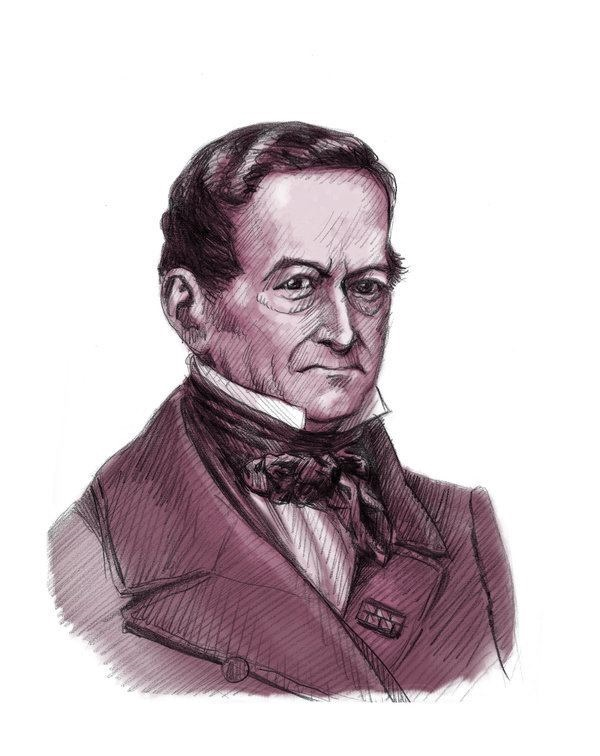
\includegraphics[scale=0.35]{figures/gottfried_achenwall.jpeg}
\vspace{-0.2cm}
\caption{Gottfried Achenwall(1719- 1772)}
\label{fig:my_label8}
\end{figure}






A palavra adquiriu o significado de coleta e classificação de dados em geral
através de Sir John Sinclair. Assim, o propósito original da
Statistik era fornecer os dados a serem usados pelo governo e
outras organizações. A coleta de dados sobre estados e localidades
continua, em grande parte através de órgãos estatísticos nacionais
e internacionais. Em particular, os censos fornecem informação
regular sobre as populações (STIGLER, 1990).\vskip0.3cm

\inic A palavra "CENSO" é derivada da palavra "CENSERE", que em Latim
significa "TAXAR". Em 1085, Guilherme, O Conquistador Normando,
solicitou um levantamento estatístico da Inglaterra, que deveria
conter informações sobre terras, proprietários, uso da terra,
empregados e animais, dos conquistados anglo-saxões. Os resultados
deste Censo foram publicados em 1086 no livro intitulado "Domesday
Book" e serviram de base para o cálculo de impostos. Na Enciclopédia Britânica, o verbete "STATISTICS" apareceu em 1797 (STIGLER, 1990).



\section{Formação da Estatística no Brasil}

\inic Um dos registros mais antigos sobre a introdução da Estatística no Brasil é uma
carta régia, datada de 8 de julho de 1800, onde o rei D. João VI solicita ao vice-rei do
Estado do Brasil a remessa de dados censitários do Brasil ao reino de Portugal.\vskip0.3cm


\inic Em 1808, D. João VI criou, a primeira instituição brasileira de ensino superior de tipo técnico, a Academia Real da Marinha, na cidade do Rio de Janeiro. Dois anos depois, é criada também a Academia Real Militar, destinada a formar oficiais da classe de engenheiros, geógrafos e
topógrafos. Nessas instituições, o ensino de disciplinas de ciências exatas seria, enfim,
encorajado no Brasil, inicialmente com as disciplinas de Física, Matemática e Química,
e posteriormente com a Estatística.\vskip0.3cm


\inic No ano de 1872, houve o primeiro censo geral da população
brasileira feito por José Maria da Silva Paranhos, conhecido como
Visconde do Rio Branco (1819-1880).\vskip0.3cm 


\inic Em 1934, foi criada a Faculdade de Filosofia, Ciências e Letras - FFCL da Universidade de São Paulo – USP, nascendo a cadeira de Estatística Geral e Aplicada pertencentes aos cursos oriundos das Ciências Sociais e Pedagogia (PEREIRA e MORETTIN, 1991).\vskip0.3cm

\inic Em 1936, tem-se a criação do Instituto Brasileiro de Geográfia e Estatística (IBGE), tornandos-se o Orgão máximo de todas as atividades estatísticas, que envolvem a sociedade Brasileira.\vskip0.3cm

\inic Em meados de 1946, a Faculdade de Filosofia, Ciências e Letras - FFCL da Universidade de São Paulo – USP, regulamentou a primeira turma de Pós-graduação em Estatística do Brasil (LOPES, 1988).\vskip0.3cm


\inic Em 1953 duas escolas iniciaram o ensino de estatística no brasil: uma no
Rio de Janeiro, a Escola Nacional de Ciências Estatística (ENCE) e
a outra conhecida como Escola de Estatística da Bahia. Só em 1972
que surge o primeiro computador brasileiro, que ajudou a dar um
grande salto na estatística.\vskip0.3cm


\inic A inclusão da Estatística no Ensino Fundamental e Médio apareceu a
partir da determinação dos Parâmetros Curriculares Nacionais
(PCN's) em 1997. De acordo com os PCN's o ensino da estatística na
escola vem ao encontro de uma sociedade que, muitas vezes, se
comunica através de gráficos, tabelas, estatísticas do trânsito,
da saúde, do jogo de futebol, etc. Assim, para que o cidadão
sobreviva e assimile este mar de estatística é necessário que
alguns conceitos sejam trabalhados desde a escola.


\section{Conceitos Básicos em Estatística}

\subsection{Definição de Estatística}

\inic É extremamente difícil definir a Estatística. O número de definições
que se encontram é extremamente grande, tendo em vista que seu domínio é
muito amplo. Assim, listam-se algumas definições formais acerca do que
seria o conceito de Estatística.\vskip0.3cm

Segundo Rao (1973), a estatística pode ser definida de uma forma
simples e objetiva. Ele define a estatística pela equação:

\begin{center}
Conhecimento Incerto + Conhecimento Sobre A Incerteza =
 Conhecimento Útil
\end{center}

Neste sentido, o objetivo da Estatística é analisar os dados
disponíveis e que estão sujeitos a um certo grau de incerteza no
planejamento e obtenção de resultados (RAO, 1999).\vskip0.3cm


Segundo Stein \& Loesch (2008), a estatística é a ciência que se
preocupa com a coleta, organização, apresentação, interpretação e
análise de dados amostrais extraídos de uma determinada
população.\vskip0.3cm

O dicionário Aurélio (2005) definiu a estatística como uma parte da matemática em que se investigam os processos de obtenção, organização e análise de dados sobre uma população ou coleção de seres quaisquer, e os métodos de tirar conclusões e fazer predições com base nesses dados.\vskip0.3cm

De acordo com Motta \& Wagner (2003), a estatística é o ramo do conhecimento que se destina ao estudo dos processos de obtenção, coleta, organização, apresentação, análise e interpretação dos dados numéricos ou variáveis referentes a qualquer fenômeno, sobre uma população ou amostra.\vskip0.3cm

É possível distinguir duas concepções para a palavra ESTATÍSTICA: no plural (estatísticas), indica qualquer coleção de dados numéricos, reunidos com a finalidade de fornecer informações acerca de uma atividade qualquer. Assim, por exemplo, as estatísticas demográficas referem-se aos dados numéricos sobre nascimentos, falecimentos, matrimônios, desquites, etc. As estatísticas econômicas consistem em dados numéricos relacionados com emprego, produção, vendas e com outras atividades ligadas aos vários setores da vida econômica. No singular (Estatística), indica a atividade humana especializada ou um corpo de técnicas, ou ainda uma metodologia desenvolvida para a coleta, a classificação, a apresentação, a análise e a interpretação de dados quantitativos e a utilização desses dados para a tomada de decisões.\vskip0.3cm

O mundo está repleto de problemas. Para resolvermos a maioria deles, necessitamos de informações. Mas, que tipo de informação Que quantidade de informações? Após obtê-las, que fazer com elas? A Estatística trabalha com essas informações, associando os dados ao problema, descobrindo como e o que coletar de dados, assim capacitando o pesquisador (ou profissional ou cientista) a obter conclusões a partir dessas informações, de tal forma que possam ser entendidas por outras pessoas. Portanto, os métodos estatísticos auxiliam o cientista social, o economista, o engenheiro, o biólogo, o agrônomo e muitos outros profissionais a realizarem o seu trabalho com mais eficiência.\vskip0.3cm

Assim, uma igualdade que pode sintetizar as considerações descritas anteriormente sobre a estatística pode ser expressa como (PADOVANI, 2012):

\begin{center}
\fcolorbox{verdemar}{white}{ESTATÍSTICA} = \fcolorbox{verdemar}{white}{CIÊNCIA} + \fcolorbox{verdemar}{white}{TECNOLOGIA} + \fcolorbox{verdemar}{white}{ARTE}
\end{center}

A estatística se divide didaticamente em duas partes: Descritiva e Inferencial


\subsection{Estatística Descritiva, Dedutiva, Analítica ou Síntese Numérica}

\inic É comum o profissional ou pesquisador defrontar-se com a situação de dispor de tantos dados que se torna difícil absorver completamente a informação que está procurando investigar. Com isso, se torna extremamente difícil captar intuitivamente todas as informações que os dados contêm, sendo necessário, portanto, que as informações sejam reduzidas até o ponto em que se possa interpretá-las mais claramente.\vskip0.3cm



A Estatística Descritiva é um ramo da estatística que aplica várias técnicas para descrever e sumariar um conjunto de dados.\vskip0.3cm

Stein e Loesch (2008) definem a estatística descritiva como o nome dado ao conjunto de técnicas analíticas utilizadas para resumir certo conjunto de todos os dados coletados numa determinada investigação.\vskip0.3cm


É a parte da estatística que procura somente descrever e avaliar certo grupo de dados seja ele a população ou a amostra. Em estatística descritiva têm-se dois métodos que podem ser usados para a apresentação dos dados: Métodos Gráficos e/ou Tabular e Métodos Numéricos, envolvendo apresentação de medidas estatísticas, entre outras.\vskip0.3cm



O objetivo da Estatística Descritiva é o de representar de uma forma concisa, sintética e compreensível, a informação contida num conjunto de dados. Esta tarefa, que adquire grande importância quando o volume de dados for grande, concretiza-se na elaboração de tabelas e de gráficos, e no cálculo de medidas ou indicadores que representam convenientemente a informação contida nos dados.\vskip0.3cm


 A descrição dos dados também tem como objetivo identificar anomalias, até mesmo resultante do registro incorreto de valores, e dados dispersos, aqueles que não seguem a tendência geral do restante do conjunto. Não só nos artigos técnicos direcionados para pesquisadores, mas também nos artigos de jornais e revistas escritos para o público leigo, é cada vez mais freqüente a utilização destes recursos de descrição para complementar a apresentação de um fato, justificar ou referendar um
 argumento.\vskip0.3cm



 Ao se condensar os dados, perde-se informação, pois não se têm as observações originais. Entretanto, esta perda de informação é pequena se comparada ao ganho que se tem com a clareza da interpretação proporcionada. Ao mesmo tempo que o uso das ferramentas estatísticas vem crescendo, aumenta também o abuso de tais ferramentas. É muito comum vermos em jornais e revistas, até mesmo em periódicos científicos, gráficos voluntariamente ou intencionalmente enganosos e estatísticas obscuras para justificar argumentos polêmicos.\vskip0.3cm


Assim, uma análise descritiva bem conduzida pode evitar vários problemas que podem ocorrer em análises mais complexas, permitindo  visualizar  muitas  características que  em  outras  análises  podem  passar  despercebidas (CAMEY, et al, 2010).






\subsection{Estatística Indutiva, Amostral ou Inferencial}

\inic Usualmente, é impraticável observar toda uma população, seja pelo custo alto seja por dificuldades operacionais. Examina-se então uma amostra, de preferência bastante representativa, para que os resultados obtidos possam ser generalizados para toda a população. Um experimento pode ter por finalidade a determinação da estimativa de um parâmetro de uma função. Toda conclusão tirada por amostragem, quando generalizada para a população, apresentará um grau de incerteza. Ao conjunto de técnicas e procedimentos que permitem dar ao pesquisador um grau de confiabilidade nas afirmações que faz para a população, baseadas nos resultados das amostras, damos o nome de Inferência Estatística.\vskip0.3cm

A estatística indutiva ou inferencial é a parte da estatística que, baseando-se em resultados obtidos da análise de uma amostra da população, procura inferir, induzir ou estimar as leis de comportamento da população da qual a amostra foi retirada. Refere-se a um processo de generalização a partir de resultados particulares. É, portanto, a parte da estatística referente a conclusões sobre as fontes de dados (CASTANHEIRA, 2005).\vskip0.3cm

%\newpage

Por exemplo, suponha-se que deseja conhecer o grau de pureza de alumina a ser exportada por um navio no porto de Manaus. Como não se pode verificar esse grau de pureza em toda a população do minério, se pega uma parte como amostra e procedem-se na mesma os testes necessários. Suponha-se que o resultado obtido nesse teste é válido para toda a população.\vskip0.3cm

Esse processo de generalização, que é caracterizado do método indutivo, está associado a uma margem de incerteza. Esta incerteza de deve ao fato de que a conclusão, que se pretende obter para toda a população analisada, baseia-se em uma amostra do total de observações. A medida de incerteza é tratada mediante técnicas e métodos que se fundamentam na teoria das probabilidades.\vskip0.3cm


Em suma, para o estabelecimento de inferências ou conclusões sobre um grupo maior (no caso a população) precisa-se usar algo além do que será visto em Estatística Descritiva. Na verdade esse algo mais seria o uso de métodos estatísticos que caracterize a área da estatística conhecida como "Estatística Indutiva" ou "Inferência Estatística".\vskip0.3cm

A estatística inferencial pode ser classificada em:

\begin{enumerate}
  \item \textbf{Estimação de Parâmetros}: inferências sobre os parâmetros (descritores matemáticos como média, desvio-padrão, proporções, risco relativo, correlação, etc.) na população em estudo baseada em estatísticas análogas (estimadores dos parâmetros) obtidos a partir da amostra.
  \item \textbf{Teste de Significância}: as probabilidades são calculadas com base em hi\-pó\-te\-ses sobre a associação exposição-desfecho na população em estudo.
\end{enumerate}


\subsection{Fenômeno Estatístico}

\inic A palavra \textbf{fenômeno} segundo o dicionário Aurélio significa qualquer modificação operada nos corpos pela ação dos agentes físicos ou quimícos. Tudo que é percebido pelos sentidos ou pela consciência. Fato de natureza moral e social, tudo que o que é objeto de experiência possível que se pode manifestar no tempo e no espaço, segundo as leis do entendimento. Assim, o fenômeno tem características próprias, ocupa lugar no tempo, têm essência e é objeto do conhecimento científico. \vskip0.3cm   

\inic O \textbf{fenômeno estatístico} é qualquer evento que se pretenda analisar, cujo estudo seja possível a aplicação do método estatístico. São divididos em três grupos:

\begin{enumerate}
  \item \textbf{Fenômeno de Massa ou Coletivo}: são aqueles que não podem ser definidos por uma simples observação. A estatística dedica-se ao estudo desses fenômenos;
  \item \textbf{Fenômeno Individual}: são aqueles que irão compor os fenômenos de massa, ou seja, do campo experimental;
  \item \textbf{Fenômeno de Multidão}: quando as características observadas para a massa não se verificam para o particular. São aqueles os quais só agem causas acidentais. A mortalidade, por exemplo, é o caso típico de um fenômeno de multidão.
\end{enumerate}


\subsection{Experimento Aleatório}

\inic Experimentos aleatórios são aqueles que, repetidos em idênticas condições, produzem resultados diferentes. Embora não se sabe qual o resultado que irá ocorrer num experimento, em geral, consegue-se descrever o conjunto de todos os resultados possíveis que podem ocorrer. As variações de resultados, de experimento para experimento, são devidas a uma multiplicidade de causas que não se pode controlar, a qual denominou acaso.

\subsection{Dado Estatístico}

Dados descrevem Fenômenos (ou Processos) ou entidades que são objetos de estudo ou análise. Desta forma, dados correspondem a atributos que podem ser caracterizados de acordo com diferentes critérios, sendo considerado a matéria-prima sobre o qual o pesquisador irá aplicar os métodos estatísticos.\vskip0.3cm

Os dados geralmente são organizados no que chamamos de \textbf{Matriz de Dados} . Se você já viu dados em uma \textbf{Planilha}, isso é uma matriz de dados. As planilhas são talvez a forma mais comum de disponibilização dos dados (Broman e Woo 2017).\vskip0.3cm



Cada linha (horizontal) representa uma observação (também chamada de unidades observacionais , casos ou assuntos). Estes são os indivíduos ou itens na amostra.\vskip0.3cm

Cada coluna (vertical) representa uma variável, a característica ou coisa que está sendo medida. Pense nas variáveis como medidas que podem variar de uma observação para outra.



\subsection{História Estatística ou História com Dados}

A maior parte da visualização de dados é feita para fins de comunicação. Temos uma visão sobre um conjunto de dados, temos um público potencial e gostaríamos de transmitir nossa visão ao nosso público. Para comunicar nossa visão com sucesso, teremos que apresentar ao público uma história clara e emocionante. \vskip0.3cm

A necessidade de uma história pode parecer perturbadora para cientistas, jornalistas e Agentes Públicos, que podem equipará-la a inventar coisas, dar uma guinada nas coisas ou exagerar nos resultados. No entanto, essa perspectiva perde o importante papel que as histórias desempenham no raciocínio e na memória.\vskip0.3cm

Os cientistas frequentemente sabem como visualizar dados sem serem grosseiramente enganosos. No entanto, eles podem não ter um senso de estética visual bem desenvolvido e podem, inadvertidamente, fazer escolhas visuais que prejudicam a mensagem desejada. Os designers, por outro lado, podem preparar visualizações que parecem bonitas, mas jogam rápido e solto com os dados. 

%(WILKE, 2019). 
\subsubsection{O Que é uma História Estatística}

Por conta própria, as estatísticas são apenas números. Eles estão em toda parte em nossa vida. Os números aparecem em histórias esportivas, relatórios sobre a economia, atualizações do mercado de ações, para citar apenas alguns. Para significar alguma coisa, seu valor para a pessoa na rua deve ser trazido à vida.\vskip0.3cm 

Uma história é um conjunto de observações, fatos ou eventos, verdadeiros ou inventados, que são apresentados em uma ordem específica para criar uma reação emocional no público.\vskip0.3cm 

Uma história estatística é aquela que não apenas recita dados em palavras. Ele conta uma história sobre os dados. Os leitores tendem a se lembrar de ideias com mais facilidade do que dos dados. Já, uma história estatística transmite uma mensagem que conta aos leitores o que aconteceu, quem fez, quando e onde aconteceu e, esperançosamente, por que e como aconteceu.\vskip0.3cm 


Uma História Estatística pode:

\begin{itemize}
    \item Fornecer conhecimento geral, algumas perspectiva, e um certo contexto;
    \item Informar o debate sobre algumas questões específicas.
\end{itemize}


Em termos jornalísticos, o número por si só não é a história. Uma história estatística mostra aos leitores o significado, a importância e a relevância das informações mais atuais. Em outras palavras, responde à pergunta: por que meu público deveria querer ler sobre isso?\vskip0.3cm 

Finalmente, uma história estatística deve conter material digno de nota. Pergunte a si mesmo: a informação é suficientemente importante e inovadora para atrair a cobertura da mídia? A mídia pode escolher um foco diferente. Mas eles têm muitos outros fatores a considerar ao escolher um enredo.

Contar histórias estatísticas é sobre:

\begin{itemize}
    \item Chamar a atenção do leitor com um título ou imagem;
    \item Fornecer a história por trás dos números de forma fácil de entender, interessante e divertida;
    \item Encorajar leitores e outros a considerar como as estatísticas podem adicionar impacto a quase todas as histórias que eles têm para contar.
\end{itemize}



\newpage
\subsubsection{Por Que Contar uma História Estatística}

Uma fonte estatística deve querer contar uma história sobre seus dados por pelo menos dois motivos. \vskip0.3cm 

Primeiro, o mandato da maioria das agências é informar o público em geral sobre a população, sociedade, economia e cultura da nação.\vskip0.3cm 

Essas informações orientarão os cidadãos na realização de seus trabalhos, na criação de suas famílias, nas compras e na tomada de muitas outras decisões.\vskip0.3cm 

Em segundo lugar, uma agência deve querer demonstrar a relevância de seus dados para o governo e o público.\vskip0.3cm 

Dessa forma, pode antecipar maior apoio público a seus programas, bem como melhorar o relacionamento com os entrevistados e maior visibilidade de seus produtos.\vskip0.3cm 

A maioria das agências conta principalmente com dois meios de comunicação de informações sobre as condições econômicas e sociais de um país e de seus cidadãos: a Internet e a Mídia.\vskip0.3cm 

A Internet tornou-se uma ferramenta importante para facilitar o acesso às informações da agência. Mais e mais membros do público acessam os dados de uma agência diretamente em seu site. Ainda assim, a maioria dos cidadãos obtém suas informações estatísticas da mídia e, de fato, a mídia continua sendo o principal canal de comunicação entre os institutos de estatística e o público em geral.\vskip0.3cm 


Uma maneira eficaz de um escritório de estatística se comunicar por ambos os meios é contar uma história estatística escrita da forma mais clara, concisa e simples possível. O objetivo da Internet é informar melhor o público por meio do acesso direto. Ao escrever para a mídia, o objetivo é obter uma cobertura positiva, precisa e informativa.\vskip0.3cm 

As estatísticas podem dizer às pessoas algo sobre o mundo em que vivem. Mas nem todo mundo é adepto de entender as estatísticas por conta própria. Consequentemente, as histórias estatísticas podem e devem fornecer uma ajuda.
Por último, mas não menos importante, a disponibilidade de estatísticas depende, em primeiro lugar, da cooperação voluntária dos respondentes da pesquisa. As agências estatísticas não podem confiar apenas em sua autoridade legal para garantir uma taxa de resposta adequada.\vskip0.3cm 


A disponibilidade de estatísticas também depende de até que ponto os entrevistados entendem que os dados servem a um propósito importante ao fornecer um espelho do mundo em que vivemos. Quanto mais uma agência estatística puder mostrar a relevância de seus dados, mais os entrevistados serão encorajados a fornecer os dados.\vskip0.3cm 

 As histórias estatísticas e os dados que elas contêm devem ser informativos e iniciar a discussão, mas nunca devem estar abertos à discussão. Em outras palavras, as informações devem ser precisas e a integridade da Fonte nunca deve ser questionada. As histórias devem ser baseadas em dados de alta qualidade que sejam adequados para descrever os problemas que abordam.\vskip0.3cm 


 As Fontes devem sempre garantir a confidencialidade dos dados de pessoas físicas ou jurídicas. Na verdade, as histórias estatísticas não podem identificar ou revelar de forma alguma dados sobre indivíduos ou empresas.\vskip0.3cm 

\subsubsection{Fluxo de Trabalho para Contar Histórias com Dados}

Nesse contexto, é sugerido um sequencia de componentes para o fluxo de trabalho para contar uma história convincente com dados.\vskip0.3cm

Existem cinco componentes principais no fluxo de trabalho necessários para contar histórias com dados

\begin{itemize}
\item[{a)}] Planeje e Esboce um Ponto Final;
\item[{b)}] Simule e Considere os Dados Planejados;
\item[{c)}] Adquira e Prepare os Dados Reais;
\item[{d)}] Explode e Entenda os Dados;
\item[{e)}] Compartilhe o que Foi Feito e o que Foi Encontrado.
\end{itemize}

Ao planejar e esbocar um ponto final, isso garante onde queremos ir, e ajuda a reduzir o aumento do escopo.\vskip0.3cm

O próximo passo é simular os dados porque isso nos obriga a entrar nos detalhes. Isso ajuda na limpeza e preparação do conjunto de dados porque nos concentra nas classes do conjunto de dados e na distribuição dos valores que esperamos.\vskip0.3cm

Adquirir e preparar os dados nos quais estamos interessados ​​é uma etapa frequentemente negligenciada do fluxo de trabalho. \vskip0.3cm

Depois de termos um conjunto de dados, queremos explorar e entender certos relacionamentos nesse conjunto de dados. Normalmente, começamos o processo com estatísticas descritivas e depois passamos para modelos estatísticos.\vskip0.3cm

Finalmente, devemos compartilhar o que foi feito e o que encontramos, com a maior fidelidade possível.\vskip0.3cm


Os elementos-chave para contar histórias convincentes com dados são:

\begin{itemize}
\item Comunicação.
\item Reprodutibilidade.
\item Ética.
\item Questões.
\item Medição.
\item Coleção de dados.
\item Limpeza de dados.
\item Análise exploratória de dados.
\item Modelagem.
\item Dimensionamento.
\end{itemize}



\newpage
\subsection{Estatísticas Vitais}

As estatísticas vitais se baseiam em dados coletados de registros de eventos vitais, como nascimento e mortes. Assim, na area de saúde os profissionais precisam ser capazes de interpretar  estatísticas vitais a fim de diagnosticar e tratar pacientes de modo eficaz.








\subsection{Hipótese Estatística}

Em termos simples, uma \textbf{hipótese} é uma resposta possível de ser testada e fundamentada para uma pergunta feita relativa ao fenômeno escolhido. O pesquisador examina a literatura sobre ao fenômeno, obtêm a maior quantidade de conhecimento possível para responder ao problema formulado. Esta tentativa de resposta é a hipótese (HIRAKATA et al, 2019).\vskip0.3cm    

As hipóteses podem ser formuladas dependendo do tipo de problema, de três maneiras


\begin{enumerate}
\item \textbf{Hipóteses Univariadas}: são os que apresentam uma variável;  
\item \textbf{Hipóteses Multivariadas}: são os que apresentam ligação entre duas variáveis;
\item \textbf{Hipóteses de Relação Casual}: são os que apresentam Relação de causa e efeito entre as variáveis.
\end{enumerate}


Existem algumas exigências para Formulação de Hipóteses:

\begin{itemize}
\item Formular hipóteses clara e precisas. Convêm estabelecer tanto as hipóteses de pesquisa, quanto as de nulidade.  
\item Indicar a importância e contribuição teórica das hipóteses.
\item Definir as variáveis, preferencialmente em termos operacionais, distinguindo as variáveis independentes e dependentes. 
\end{itemize}

Para Hirakata (et al, 2019) a hipótese estatística é uma suposição formulada a respeito dos parâmetros de uma ou mais populações e é testada a partir dos resultados amostrais. 

\subsubsection{Teste de Hipóteses}

O teste de hipóteses é um método de averiguação sobre a veracidade de uma afirmação, associado a um risco máximo de erro. Em termos estatísticos, um teste de hipóteses é uma regra de decisão para aceitar ou rejeitar uma hipótese, com base nas informações fornecidas pelos dados coletados em uma amostra (CALLEGARI-JACQUES, 2013).\vskip0.3cm



 %Soares JF, Siqueira AL. Introdução à estatística médica. Belo Horizonte: Coopmed; 1999


% Hulley SB, Cummings SR, Browner WS, Grady D, Hearst N, Newman TB. Delineando a pesquisa clínica: uma abordagem epidemiológica. Porto Alegre: Artmed; 2003.


% Mancuso ACB, Castro SMJ, Guimarães LSP, Leotti VB, Hirakata VN, Camey AS. Estatística descritiva: perguntas que você sempre quis fazer, mas nunca teve coragem. Clin Biomed Res. 2018;38(4):414-8

As especificações sobre os parâmetros denominam-se hipóteses estatísticas, formuladas da seguinte forma:

\begin{itemize}
\item Hipótese Nula, da Nulidade ou Hipótese Básica, cujo o símbolo é representado da seguinte forma $H_{0}$ (Agá-zero).
\item Hipótese Alternativa, simbolizando como segue: $H_{1}$ ou $H_{A}$.
\end{itemize}

A hipótese de nulidade sempre significa \textbf{inocência}, ou seja, não há diferença entre os parâmetros das populações submetidas às observações ou aos experimentos. A hipótese alternativa sempre é \textbf{culpada}, de haver diferença entre os parâmetros dos universos em questão e contradiz a de nulidade.\vskip0.3cm



A hipótese nula é sempre a hipótese a ser examinada. As hipóteses estatísticas que podem ser testadas numericamente são utilizadas nos seguintes casos:

\begin{itemize}
\item testar a diferença entre dois ou mais grupos em relação a uma ou mais características.
\item testar a associação entre duas ou mais variaveis em um grupos ou entre vários grupos. 
\item testar a estimação de pontos das características de uma amostra ou população.
\end{itemize}


\newpage
\subsection{Tipos de Pesquisa Científica}

\inic Existem várias maneiras de classificar uma pesquisa, e os autores não são unânimes quanto à padronização desta classificação. Neste contexto, sugere-se uma maneira simples e objetiva.\vskip0.3cm 

\begin{quadro}[h!tp]
    \centering
    \caption{Equema geral dos Tipos de Pesquisas, segundo a sua classificação (IBGE, 2003).}
    \begin{tabular}{|l|l|}
    \hline \hline
    CLASSIFICAÇÃO                & TIPOS DE PESQUISAS   \\    
    \hline\hline
     Quanto à Finalidade         & Básica/Aplicada \\
     \hline
     Quanto à Natureza           & Observacional/Experimental  \\
     \hline
    Quanto à Forma de Abordagem  & Qualitativa/Quantitativa \\
    \hline
     Quanto aos Objetivos        & Exploratória/Explicativa \\
     \hline
    Quanto aos Procedimentos Técnicos     & Bibliográfica/Documental             \\
       \hline     
    Quanto ao Desenvolvimento    & Transversal/Longitudinal              \\
  \hline\hline
    \end{tabular}
    %\fonte{Autor: FONTELLES, 2011.}
\end{quadro}






\textbf{Quanto à Finalidade}: 

\begin{itemize}
\item \textbf{Pesquisa Básica ou Fundamental}: é aquela cujo objetivo é adquirir novos conhecimentos que possam contribuir para o avanço da ciência. Neste tipo de pesquisa, o investigador acumula conhecimentos e informações que podem, eventualmente, levar a resultados acadêmicos ou aplicados importantes. Alguns autores incluem, nesta categoria, as pesquisas realizadas na area acadêmica, aquelas realizadas na instituição de ensino superior como parte das atividades de ensino-aprendizagem, tal como nos trabalhos de conclusão de curso (KENDALL, 2003). 
\item \textbf{Pesquisa Aplicada ou Tecnológica}:é o tipo de pesquisa cujo objetivo é produzir conhecimentos científicos para aplicação prática voltada para a solução de problemas concretos, específicos da vida moderna. È a pesquisa que, além de produzir conhecimento, gera novos processos tecnológicos e novos produtos, com resultados práticos imediatos em termos econômicos e na melhoria da qualidade de vida (BOISSEL, 2004).
\end{itemize}

\textbf{Quanto à Natureza}: 

\begin{itemize}
\item \textbf{Pesquisa observacional}: O Pesquisador atua meramente como expectador de fenômeno ou fatos, sem, no entanto, realizar qualquer intervensão que possa interferir no curso natural e/ou no desfecho dos mesmos, embora possa, neste meio tempo, realizar medições, análises e outros procedimentos para coleta de dados (HULLEY et al, 2003).
\item \textbf{Pesquisa Experimental}: é qualquer pesquisa que envolve algum tipo de experimento. Neste caso, o pesquisador participa ativamente na condução do fenômeno, processo ou do fato avaliado, isto é, ele atua na causa, modificando-a, e avalia as mudanças no desfecho. Neste tipo de pesquisa, o investigador seleciona as variáveis que serão estudadas, define a forma de controle sobre elas e observa o efeitos sobre o objeto de estudo, em condições pré-estabelecidas. Assim, pelo fato das variáveis, ou da variável, poderem ser manipuladas pelo pesquisador, equívocos e vieses praticamente  desaparecem, sendo, por esta razão, considerada como o melhor tipo de pesquisa científica, pois proporciona maior confiabilidade em seus resultados. Os mais tradicionais tipos de delineamento da pesquisa experimental são os estudos controlados (duplo cego, randomizado ou aleatório, não-randomizado, autocontrolado e com controle externo) e não-controlados (SILVA, 2004). 
\end{itemize}


\textbf{Quanto á Forma de Abordagem}: 

\begin{itemize}
\item \textbf{Pesquisa Qualitativa}: é o tipo de pesquisa apropriada para quem busca o atendimento de fenômenos complexos específicos, em profundidade, de natureza social e cultural, mediante descrições, intepretações e comparações, sem considerar os seus aspectos numéricos em termos de regras matemácticas e estatísticas. Diferente da quantitativa, a pesquisa qualitativa é mais participativa, porém menos controlável e, por esta razão, tem sido questionada quanto a sua validade e confiabilidade (SILVA, 2001) e (SILVA, 2004).
\item \textbf{Pesquisa Quantitativa}: é aquela que trabalha com variáveis expressas sob a forma de dados numéricos e emprega rígidos recursos e técnicas estatísticas para classificá-los e análisá-los, tais como a porcentagem, a média, o desvio-padrão, o coeficiente de correlação e as regressões, entre outros. Em razão de sua maior precisão e coanfiabilidade, os estudos quantitativos são mais indicados para o planejamento de ações coletivas, pois seus resultados são passíveis de generalização, principalmente quando as amostras pesquisadas representam, com fidelidade, a população de onde retiradas (SILVA, 2001; SILVA, 2004).
\end{itemize}


\textbf{Quanto aos Objetos}: 

\begin{itemize}
\item \textbf{Pesquisa Exploratória}: este tipo de pesquisa visa a uma primeira aproximação do pesquisador com o tema, para torná-lo mais familiarizado com os fatos e fenômenos relacionados ao problema a ser estudado. No estudo, o investigador irá buscar subsídios, não apenas para determinar a relação existente, mas, sobretudo, para conhecer o tipo de relação (SILVA, 2011; SILVA, 2004) e (MARCONE, 2005).
\item \textbf{Pesquisa Explicativa}: tem por objetivo central explicar os fatores determinantes para a ocorrência de um fenômeno, processo ou fato, ou seja, visa explicar o porquê das coisas. É uma consequência lógica da pesquisa exploratória.(SILVA, 2011; SILVA, 2004) e (MARCONE, 2005).
\end{itemize}


\textbf{Quanto aos Procedimentos Técnicos}: 

\begin{itemize}
\item \textbf{Pesquisa Bibliográfica}: sua base é a analise de material já publicado. É utilizada para compor a fundamentação teórica a partir da avaliação atenta e sistemática de livros, periódicos, documentos, textos, mapas, fotos, manuscritos e, até mesmo, de material disponibilizado na internet etc. Este tipo de pesquisa fornece o suporte a todas as fases de um protocolo de pesquisa, pois auxilia na escolha do tema, na definição da questão da pesquisa, na determinação dos objetos, na formulação das hipóteses, na fundamentação da justificativa e na elaboração do relatório final.
\item \textbf{Pesquisa Documental}: é o tipo de pesquisa que tem o levantamento de documentos como base. É uma valiosa técnica de coleta de dados qualitativos. Assemelha-se à pesquisa bibliográfica, a qual utiliza a contribuição fornecida por diversos autores sobre um determinado assunto, enquanto na pesquisa documental, a coleta de informações é realizada em materiais que não receberam qualquer tipo de análise crítica. Neste tipo de pesquisa, os documentos consultados são, geralmente, classificados  como fontes primárias e fontes secundárias. No primeiro caso, são fontes cuja a origem remonta a época que se está pesquisando, ainda não analisados e que, frequentemente, foram produzidas pelas próprias pessoas estudadas, tais como correspondência, diários, textos literários e outros documentos mantidos em orgãos públicos e instituições privadas de qualquer natureza; no segundo, corresponde às fontes cujos trabalhos escritos se baseiam na fonte primária e tem como característica o fato de não produzir informações originais mas apenas uma análise, ampliação e comparação das informações contidas na fonte original.
\item \textbf{Pesquisa de Laboratório}: a principal característica é a sua realização em ambiente controlado, seja um laboratório ou não. Estas pesquisas, que geralmente são experimentais, adotam ambientes de simulação para reproduzir o fenômeno objeto do estudo, além de utilizar-se de instrumentos específicos e precisos de coleta e análise de material.
\item \textbf{Pesquisa de Campo}: uma pesquisa de campo procura coletar dados que lhe permitam responder aos problemas relacionados a grupos, comunidades ou instituições, com o objetivo de compreender os mais diferentes aspectos de uma determinada realizada, sendo mais frequentemente utilizada pelas áreas das ciências humanas e sociais mediante técnicas observacionais e com a utilização de questionários para a coleta de dados. 
\end{itemize}

\textbf{Quanto ao Desenvolvimento no Tempo}: 

\begin{itemize}
\item \textbf{Pesquisa Transversal e Longitudinal}: a diferença entre as duas é o intervalo de tempo que o pesquisador utiliza para a condução da pesquisa. No estudo transversal (ou seccional), a pesquisa é realizada em um curto período de tempo, em um determinado momento, ou seja, em um ponto no tempo, tal como agora, hoje. Mais dinâmica que a transversal, a pesquisa longitudinal pode ser classificada como prospectiva e retrospectiva e tem como subtipos o estudo caso-controle e o estudo de coorte prospectivo. 
\item \textbf{Pesquisa Prospectiva e Retrospectiva}: nesta classificação, a diferença é o sentido da condução da pesquisa em relação ao tempo de sua realização. Na pesquisa prospectiva, o estudo é conduzido a partir do momento presente e caminha em direção ao futuro. Já na retrospectiva, o estudo é desenhado para explorar fatos do passado, podendo ser delineado para retornar, do momento atual até um determinado ponto no passado.Um exemplo são os estudos caso-controle, em que o pesquisador pode marcar um ponto no passado e conduzir a pesquisa até o momento presente, pela  análise documental, tal como acontece no estudo do tipo coorte retrospectiva (coorte histórica). 
\end{itemize}


\newpage
\subsection{População e Censo}

\begin{enumerate}
  \item \textbf{População ou Universo Amostral} : É o conjunto de todos os elementos relativos
  a um determinado fenômeno (ex: pessoas, animais, vegetais, ou objetos) que possuem ao menos uma característica em comum (de carater demográfico, clínico e temporal)
  entre todos os seus componentes , sendo um conjunto universo podendo ser
  finita ou infinita. Esta cacterística deve delimitar corretamente quais
  são os elementos da população que podem ser animados ou inanimados (SILVA, 2011).\vskip0.3cm

 As populações são classificadas segundo alguns critérios (AIRES, 2013).
 \begin{enumerate}
   \item \textbf{Tamanho}: finitas e infinitas;
   \item \textbf{Número de variáveis}: univariada, bivariadas e multivariadas;
   \item \textbf{Aspecto Existencial}: populações hipotéticas ou conceituais;
   \item \textbf{Objetivo da Investigação}: descritivo e analítico e combinado;
   \item \textbf{Obtenção dos Parâmetros}: censitários, inferenciais, alvo, emoldurado e de respondentes;
 \end{enumerate}



  \item \textbf{Censo} : É a coleta total das informações sobre a
  população em estudo, sendo realizado a cada 10 anos pelo Instituto
  Brasileiro de Geografia e Estatística (IBGE). A população é contada
  em todo o território do Brasil e os resultados são usados
  pelo governo no desenvolvimento de políticas públicas e na
  destinação dos fundos governamentais para as unidades federativas.
  Em 1872, foi realizado o primeiro Censo Nacional no Brasil, já o último foi em 2010.
\end{enumerate}

\subsection{Dados, Unidade, Amostra, Elemento e Amostragem}

\begin{enumerate}

\item \textbf{Dados Estruturados} : em que a informação se ajusta às estruturas
usuais de bases de dados, relativamente fáceis de armazenar e analisar.
Exemplos usuais de dados numéricos ou não, que podem ser dispostos
em matrizes de dados;

\item \textbf{Dados Não Estrturados}: tudo o que não se encaixa no item anterior, como arquivos de textos, páginas da web, emails, mídias sociais etc.

\item \textbf{Unidade} : É qualquer elemento individual da população;

\item \textbf{Amostra} : É uma parte ou subconjunto da população,
ou seja, são subconjuntos de elementos da mesma, de modo que
represente as características totais da população como se fosse
uma fotografia da mesma;

\item \textbf{Elemento} : O elemento sgnifica cada uma das
unidades observadas no estudo, no qual, após a determinação dos
elementos pergunta-se: o que fazer com estes? Pode-se medí-los,
observá-los, contá-los surgindo um conjunto de respostas que
receberá a denominação de variável;

 \item \textbf{Amostragem} : É o
processo ou método de coleta das informações de parte da
população, mediante alguns processos adequados de seleção.
\end{enumerate}

\subsection{Erro, Fração Amostral, Nível de Confiança, P-valor e Poder}


\begin{enumerate}
\item \textbf{Erro Amostral} : É a diferença entre um resultado amostral e o verdadeiro resultado populacional; tais erros resultam de flutuações amostrais aleatórias. Não se pode evitar a ocorrência do erro amostral, porém pode-se limitar seu valor através da escolha de uma amostra de tamanho adequado. O erro amostral é reduzido pelo aumento do tamanho da amostral e medido pelo erro padrão. O erro amostral é também, denominado de erro casual, pois ocorre nas amostras aletórias e é decorrente:

\begin{itemize}
\item Da variação de um indivíduo em relação a outro indivíduo;
\item De um mesmo indivíduo em momentos diferentes;
\item De um observador para outro observador, em relação ao mesmo indivíduo ;
\item Dos instrumentos de medição, como os aparelhos de aferir a pressão arterial, a dosagem alcoólica (etilômetro), etc;
\end{itemize}


\item \textbf{Fração Amostral} : É o quociente entre a dimensão da
amostra e o tamanho da população; 
\item \textbf{Nível de
Confiança} : nível de confiança p ou, simplesmente, confiança p de
uma medida é a probabilidade P de que o valor apresentado esteja
correta. O nível de confiança de uma pesquisa é estabelecido de
comum acordo entre o cliente e o instituto, entretanto, o mais
usual é trabalhar com intervalos de $95\%$ de confiança.

\newpage
\item \textbf{P-valor}: O valor de P mede a probabilidade de que
a hipótese nula (a ausência de um padrão) seja verdadeira. Desse modo, valores de P muito
próximos de zero indicam que a probabilidade de que a hipótese nula seja verdadeira é muito
baixa e que é possível considerar cenários alternativos, ou seja, aceitar a hipótese alternativa.
\item \textbf{Poder} : o poder é a probabilidade de rejeição da hipótese nula quando ela é verdadeiramente falsa ou, de modo equivalente, a conclusão de que a hipótese alternativa é verdadeira quando o é de fato. O poder é calculado em cima do erro tipo II e relacionado com o tamanho da amostra.
\end{enumerate}




\subsection{Parâmetro, Estimador e Estimativa}

\begin{enumerate}
\item \textbf{Parâmetro} : É uma medida numérica que descreve alguma característica na população.

\item \textbf{Estimador} : A combinação dos elementos da amostra,
construída com a finalidade de representar ou estimar um
parâmetro de interesse na população denomina-se estimador.
Normalmente, é representado por uma fórmula. Assim, um
estimador é uma medida que descreve uma característica na amostra.


\item \textbf{Estimativa} : É um valor numérico aproximado do
parâmetro e é calculado com o uso da amostra, ou seja, uma
estimativa é um valor particular de um estimador, utilizada para descrever características de uma amostra.
\end{enumerate}


A estatística, quando aplicada em algumas áreas do conhecimento,
recebe uma denominação diferente conforme a natureza ou
característica do fenômeno em estudo. Assim, observa-se alguns
exemplos.


\newpage
\subsection{Conceitos de Estatística em outras Áreas}
\subsubsection{Bioestatística}

É a metodologia estatística aplicada às ciências biológicas, com a finalidade em planejar, coletar, organizar, resumir, analisar e interpretar os dados,
permitindo tirar conclusões biológicas sobre populações a partir do estudo
de amostras.\vskip0.3cm

Conforme Padovani (2012) a denifição de bioestatística pode ser expressa da seguinte forma:

\begin{center}
\fcolorbox{verdemar}{white}{BIOESTATÍSTICA} = \fcolorbox{verdemar}{white}{VIDA} + \fcolorbox{verdemar}{white}{ESTATÍSTICA}
\end{center}


\subsubsection{Geoestatística} 

A Geoestatística tem por objetivo a
caracterização espacial de uma variável de interesse por meio do
estudo de sua distribuição e variabilidade espaciais, com
determinação das incertezas associadas.\vskip0.3cm


\subsubsection{Econometria} 

È um conjunto de ferramentas estatísticas com o objetivo de entender a relação entre variáveis econômicas através da aplicação de um modelo estatístico.\vskip0.3cm

O conceito de econometria é as vezes confundido com economia matemática, o sufixo "metria"
está relacionado a medição de dados econômicos, abordando estudos de observações empíricas
através de métodos estatísticos de estimação e testes de hipóteses. O ramo da economia
matemática, por sua vez, se destina a aplicação da matemática a aspectos puramente teóricos
da análise econômica, preocupando-se muito pouco, ou quase nada, com problemas estatísticos
como erros de medição das variáveis que estão sendo investigadas.\vskip0.3cm


\subsubsection{Quimiometria} 

Quimiometria é a ciência relacionada a
medidas realizadas em um sistema ou processo químico, obtendo
informações sobre o estado do sistema através da aplicação de
métodos estatísticos (FERREIRA, 2015).\vskip0.3cm

\subsubsection{Psicometria} 

È um ramo da Psicologia e que se caracteriza por expressar (observar) o fenômeno psicológico através do número, em vez da pura descrição verbal (PASQUALI, 2013).  
\vskip0.3cm

\subsubsection{Jurimetria} 

A jurimetria serve de ferramenta para a compreensão do universo de processos e fatos jurídicos. Quando estudamos uma única norma geral e abstrata, por exemplo, um artigo de lei, há ferramentas apropriadas para a sua descrição, como a história, a gramática ou a lógica. Já o estudo de populaçőes demanda a utilização de outras áreas do conhecimento capazes de descrever de forma resumida as suas tendęncias centrais e a sua variabilidade: a estatística e a probabilidade. Diferentemente das normas abstratas, os processos e fatos jurídicos surgem em populaçőes numerosas, mas cujas características podem ser sumarizadas . A jurimetria é, portanto, a disciplina resultante da aplicação de modelos estatísticos na compreensão dos processos e fatos jurídicos (NUNES, 2019).\vskip0.3cm

\subsubsection{Contabilometria} 

Representa a utilização de metodologia científica de métodos quantitativos (Matemática, Estatística e Informática) na Contabilidade.



\subsubsection{Sociometria}

A palavra Sociometria, derivada do latim, é resultante da junção das palavras \textbf{Socius} (social) e \textbf{Metrum} (medida). Foi desenvolvida pelo Médico, \textbf{Jacob Levy Moreno(1889-1974)} nos seus estudos sobre a relação entre estruturas sociais e bem-estar psicológico.\vst

Jacob trabalhou de forma paralela, com psicólogia, filósofia, dramaturgia, nascido na Romênia, crescido na Áustria (Viena) e naturalizado americano, é considerado o criador do \textbf{Psicodrama} e pioneiro no estudo da Terapia em Grupo. 

\subsubsection{Antropometria}
Parte da estatística que estuda as medições das populações sob o ponto de vista de crescimento, peso, estatura e envelhecimento (WHIPPLE, 1923).


\subsubsection{Patometria}

Parte da estatística que estuda as patologias do ser humano e suas morbidade. Do ponto de vista da quantificação de doenças, é o processo pelo qual os sintomas são mensurados e expressos em unidades que permitam comparações objetivas.



\subsection{Estatística Experimental}

A estatística experimental estuda o planejamento, execução, análise e interpretação de experimentos, e se caracteriza como um trabalho planejado, obdecendo a determinados princípios básicos, visando comparar efeitos de tratamentos.\vskip0.3cm

Peres e Saldiva(1982), estabelecem que uma pesquisa experimental, estatisticamente bem planejada, consiste em definir as etapas a serem cumpridas, as quais dependem de um perfeito entedimento entre o pesquisador e o estatístico. As principais etapas a serem consideradas no Planejamento de um experimento:

\begin{itemize}
    \item Enunciação do Problema com Formulações das Hipóteses;
    \item Comparar as Médias;
    \item Definição dos fatores (variáveis independentes) e seus respectívos níveis;
    \item Definição da Unidade Experimental ou Unidade de Observação;
    \item Definição das Variáveis que serão medidas nas unidades de observação;
    \item Estabeleciment dos Procedimentos para alocação dos diferentes tratamentos (combinação de níveis de fatores) às unidades experimentais ou vice-versa.
\end{itemize}

Estes itens basicamente sintetiza o que se denomina Planejamento Estatístico de Experimentos, pois se trata das regras que associam as unidades experimentais ou tratamentos, e por consequencia, determinam os diferentes delineamentos experimentais.   


\newpage
\subsection{Variável Estatística}

Inicialmente, será apresentado e discutido questões referentes ao conceito Medida e a classificação de variáveis.\vskip0.3cm

De forma didática, em termos estatísticos, a palavra \textbf{Medida} é utilizada em referência aos resultados de uma variável aleatória observada (ou mensurada) na amostra de um determinado evento ou estudo estatístico. A diferença entre ser \textit{dependente} ou \textit{independente} está na relação da variável (medida) em questão com as demais (LEOTTI et al, 2019).\vskip0.3cm

As variáveis são todas e qualquer \textbf{atributo}, \textbf{características}, \textbf{propriedades} ou \textbf{condição} que podem ser mensuradas, medidas ou observadas em cada elemento na população, sob as mesmas condições. Toda variável é passível de ser modificada, ou seja, apresentar variação em seus valores de indivíduo a individuo ou no mesmo indivíduo de um momento a outro (PINHEIRO et al, 2009).\vskip0.3cm 

As variáveis podem ser classificadas de diversas formas, na área Médica, por exemplo, é comum classificar uma variável em  \textit{dependente}, freqüentemente denominada de \textbf{Desfecho de interesse ou Resposta}, e variável \textit{independente}, como \textbf{Preditora, Explicativa, Exposição, Fator ou Covariáveis em estudo}. \vskip0.3cm 


A variável de pendente é um fenômeno que aparece, desaparece, aumenta ou diminui conforme as mudanças ocorridas em ao menos uma outra variável.\vskip0.3cm 

A variável independente ou preditora é aquela que, em teoria, causa o efeito que se procura confirmar, já a variável dependente é a que mede o efeito sofrido.\vskip0.3cm



A classificação das variáveis é muito importante, pois diferentes tipos de variáveis exigem tratamentos estatísticos específicos, por exemplo: qual é a idade média das mulheres
que exercem atividade remunerada? Qual é a proporção (percentual) de mulheres que trabalham fora o dia todo?
\vskip0.3cm



\inic De modo geral, as varáveis estatística pode ser classificadas em \textbf{Qualitativas ou Categóricas} e \textbf{Quantitativas ou Numéricas}.\vskip0.3cm

\inic As Variáveis Qualitativas ou Categóricas são aquelas que estão associadas à qualidade ou quando seus valores forem expressos em forma de atributos, conhecidos também como categorias da variável, tendo características não numéricas. As variáveis qualitativas são classificadas segundo seu nível ou escala de medidas em \textbf{Nominal} e \textbf{Ordinal}.\vskip0.3cm


\begin{enumerate}
\item \textbf{Variável Qualitativa Nominal} : são aquelas cuja variável envolve fre\-qüên\-cias e não medidas propriamente ditas, nesse tipo de variáveis, o indivíduos são agrupados em categorias e conta-se a freqüência com que ocorrem. Estas categorias são sempre em número limitado e não muito grande, são exclusivas entre si e seu conjunto constitui todas as possibilidades da variável. As variáveis nominais são geralmente aquelas, cujas categorias são simples rótulos, não havendo um sentido de comparação ou ordenação, ou seja, não possuem nenhuma relação hierárquica entre si. Esse tipo de variável compõe-se de duas ou mais categorias, quando possui apenas duas categorias ou estados, é chamada de \textbf{Dicotômica ou Binária}, por exemplo;


    $$
    Genero
    \left\{
    \begin{array}{ll}
    Masculino & \hbox{ } \\
    Feminino & \hbox{ }
    \end{array}
    \right.
  Gravidez
    \left\{
    \begin{array}{ll}
    Positivo & \hbox{ } \\
    Negativo & \hbox{ }
    \end{array}
    \right.
    Habito \ Etilico
    \left\{
    \begin{array}{ll}
    Sim & \hbox{ } \\
    Nao & \hbox{ }
    \end{array}
    \right.
    $$


    $$
    Frota
    \left\{
    \begin{array}{ll}
    Adimplente    & \hbox{ } \\
    Inadimplente  & \hbox{ }
    \end{array}
    \right.
     Acidentes
    \left\{
    \begin{array}{ll}
    Fatal     & \hbox{ } \\
    Nao \ Fatal & \hbox{ }
    \end{array}
    \right.
    $$


Entretanto, as variáveis nominais comumente apresentam três ou mais categorias sendo então, chamadas de \textbf{poliatômicas ou polinomiais}, por exemplo:


    $$
    Raca
    \left\{
    \begin{array}{ll}
    Branco  & \hbox{ } \\
    Negro   & \hbox{ } \\
    Pardo   & \hbox{ } \\
    Cafuso  & \hbox{ }
    \end{array}
    \right.
    Religiao
    \left\{
    \begin{array}{ll}
    Catolico   & \hbox{ } \\
    Evangelico & \hbox{ } \\
    Adventista & \hbox{ } \\
    Budista    & \hbox{ }
    \end{array}
    \right.
    Grupo \ \  Sanguineo
    \left\{
    \begin{array}{ll}
    A    & \hbox{ } \\
    B    & \hbox{ } \\
    AB   & \hbox{ } \\
    O    & \hbox{ }
    \end{array}
    \right.
    $$

    $$
     Estado \ \ Civil
    \left\{
    \begin{array}{ll}
    Solteiro    & \hbox{ } \\
    Casado      & \hbox{ } \\
    Separado    & \hbox{ } \\
    Viúvo       & \hbox{ } \\
    \end{array}
    \right.
    $$



\inic Muitas classificações principalmente nas pesquisas médicas são avaliadas de acordo com a escala nominal, os resultados de um tratamento médico ou procedimento cirúrgico, assim como a presença de possíveis fatores de risco ou de exposição, em geral são descritos como ocorrentes ou não-ocorrentes.\vst 



Trata-se de um nível de mensuração restritivo em termos de possibilidades do uso de técnicas estatísticas, uma vez que não são possíveis operações aritméticas com seus valores. Os dados nominais são descritos geralmente em termos de percentagens ou proporções. As tabelas de contingência e os gráficos de barras são usados com mais freqüência para mostrar esse tipo de informação.


%\newpage
\item \textbf{Variável Qualitativa Ordinal}: são variáveis nas quais suas categorias obedecem a uma ordenação natural, ou seja, refere-se a uma variável que classifica os indivíduos de acordo com as categorias de uma característica, as quais podem ser ordenadas por algum sistema de graduação. Neste nível de escala, não só é possível identificar diferentes categorias, mas também reconhecer graus de intensidade entre elas, o que possibilita uma ordenação das várias categorias, porém, é necessário que a gradação seja inerente a variável e não imposta por conveniência do pesquisador. Uma característica importante das escalas ordinais é que, embora exista a ordem entre as categorias, a diferença entre duas categorias adjacentes não é a mesma em toda a escala. Assim, como nas escalas nominais, as percentagens e proporções são freqüentemente usadas com as escalas ordinais, podendo ser resumido algumas vezes pelo valor Mediano, e as mesmas tabelas e gráficos usados para exibir os dados nominais também podem ser usados com os dados ordinais.
\end{enumerate}


$$
    Escolaridade
    \left\{
    \begin{array}{ll}
    Fundamental  & \hbox{ } \\
    Medio        & \hbox{ } \\
    Superior     & \hbox{ } \\
    Posgraduado  & \hbox{ }
    \end{array}
    \right.
    Faixa \ Etaria
    \left\{
    \begin{array}{ll}
    18 \ a \ 25   & \hbox{ } \\
    26 \ a \ 30   & \hbox{ } \\
    31 \ a \ 35   & \hbox{ } \\
    36 \ a \ 40    & \hbox{ }
    \end{array}
    \right.
    $$



As \textbf{Variáveis Quantitativas ou Numéricas} são aquelas cujos valores são de\-cor\-ren\-tes de dados expressos de forma numérica, pois medem a quantidade de alguma coisa. As variáveis quantitativas são classificadas segundo seu nível ou escala de medidas em \textbf{Discreta (escala de razão)} e \textbf{Contínuas (escala intervalar)}.


\begin{itemize}
  \item \textbf{Variável Quantitativa Discreta}: são variáveis que resultam da mensuração de quantidades cujos valores somente são expressos ou assumem valores inteiros, ou seja, são aqueles que não podem assumir qualquer valor dentro de um intervalo valido para a variável, sendo as variáveis mais simples e normalmente usadas, são apuradas ou está associada a processos de contagem;

 \begin{itemize}
   \item Número de Sintomas de uma Doença;
   \item Número de Gols em uma Partida de Futebol;
   \item Número de Filhos;
   \item Número de Carros;
   \item Número de Empregados.
 \end{itemize}
  \item \textbf{Variável Quantitativa Contínua}: são variáveis que podem assumir qualquer valor numérico dentro de certo intervalo de variação possível, geralmente as variáveis continuas estão associadas à medição, por exemplo.
\begin{itemize}
  \item Temperatura; Pressão; Volume;
  \item Liquidez; Rentabilidade; Solvência;
  \item Inteligência, Ansiedade; Depressão;
  \item Altura; Peso; Comprimento; Diâmetro;
\end{itemize}
\end{itemize}



\newpage
\section{Conceitos Modernos em Estatística}

\subsection{\textit{Big Data} (Megadados ou Macrodados)}


O termo big data surgiu em meados de 1997, que foi inicialmente utilizado para nomear conjuntos de dados não ordenados em rápido crescimento. Nas últimas décadas, os conjuntos de dados têm crescido de forma exponencial.


\vspace{-1.9cm}
\begin{figure}[H]
\centering
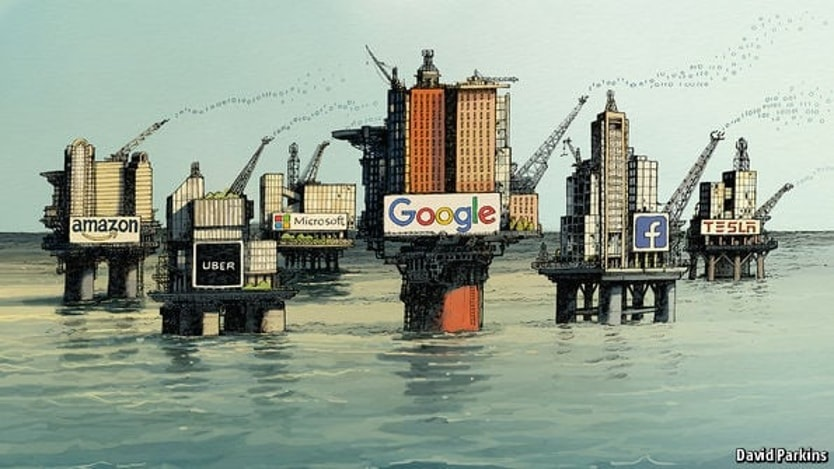
\includegraphics[scale=0.5,height=220pt,width=15cm]{figures/dados1.jpeg}
\caption{Exemplo sobre as Principais Bases de Dados Mundiais}
\label{fig:my_label8}
\end{figure}

Big data é um termo geral para qualquer coleção de conjuntos de dados tão grandes ou complexos que torna-se difícil processá-los usando técnicas tradicionais de gerenciamento de dados.\vskip0.3cm

Em 2010, o Apache Hadoop definiu big data como “conjuntos de dados que não podem ser capturados, gerenciados e processados por computadores em geral dentro de um escopo aceitável”





\subsection{Data Science (Ciência de Dados)}

A ciência de dados envolve o uso
métodos para analisar grandes quantidades de dados e extrair o conhecimento que eles contêm.
Você pode pensar na relação entre big data e ciência de dados como sendo
a relação entre o petróleo bruto e uma refinaria de petróleo. 



%\subsection{Business Intelligence}





\subsection{Machine Learning (Apredizado de Máquina)}


O termo aprendizado de máquina é um método de análise de dados que automatiza a construção de modelos analíticos. É um subcampo ou ramo da inteligência artificial baseado na idéia de que sistemas podem aprender com dados, identificar padrões e tomar decisões com o mínimo de intervenção humana.\vskip0.3cm

Em 1959, Arthur Samuel definiu aprendizado de máquina como o "campo de estudo que dá aos computadores a habilidade de aprender sem serem explicitamente programados.\vskip0.3cm

Um algoritmo de aprendizado é um conjunto de instruções que devem ser compreendidas
por um computador para que ele possa aprender com os dados (Mitchell, 1997).



\subsection{Web Scraping (Coleta de Dados Web)}

A coleta de dados web, ou raspagem web, é uma forma de mineração que permite a extração de dados de sites da web convertendo-os em informação estruturada para posterior análise.


\section{Fases ou Etapas de um Levantamento ou Método Estatístico}

\inic A pesquisa científica é a aplicação prática de um conjunto de procedimentos objetivos, utilizanados por um pesquisador (cientista), para o desenvolvimento de um experimento, a fim de produzir um novo conhecimento, além de integrá-los aqueles pré-existentes. (BARROS et al, 2002). Constituindo-se portanto, em etapas ordenadamente dispostas, de maneira lógica e racional, as quais o pesquisador deverá conhecê-las para aplicá-las convenientemente. (SILVA e MENEZES, 2001). 
\vskip0.3cm


Ao realizar um estudo experimental qualquer ou estatístico completo em determinada população ou em uma parte da mesma (no caso amostra), o trabalho estatístico que se realizará, deverá passar por várias fases onde serão desenvolvidos até se chegar aos resultados finais esperados.\vskip0.3cm

Assim, um levantamento ou trabalho estatístico consiste em um
método que pode ser estruturado de tal forma que possibilite seu
desenvolvimento nas seguintes fases ou etapas:
\textbf{Planejamento}, \textbf{Coleta de Dados}, \textbf{Apuração
ou Contagem de Dados}, \textbf{Organização, Exposição ou
Apresentação de Dados}, \textbf{Análise ou Interpretação de
Dados}, \textbf{Relatório Final e Divulgação dos Resultados}.


\subsection{Planejamento}

O planejamento é a etapa inicial do trabalho estatístico, sem duvida representa uma das mais importantes fases do levantamento, nessa etapa procura-se reunir tudo o que existe publicado sobre o fe\-nô\-me\-no a ser estudado, analisando experiências de trabalhos anteriores. Inicialmente, defini-se com clareza o objetivo da pesquisa ou o problema que se pretende pesquisar e, qual é exatamente o objetivo que se deseja alcançar. Porém, não é suficiente saber o que se pretende pesquisar. È também necessário saber onde será realizada a pesquisa: em que local, com que tipo de pessoas (ou objetos), em que época (dias, horários) e assim por diante. Assim, uma vez definido e delimitado o problema, é preciso estar atento a uma série de questões.\vskip0.3cm


O planejamento de uma pesquisa envolve as seguintes etapas:


 \begin{itemize}
   \item \textbf{Formulação do Tema e dos Objetivos Gerais e Específicos}: 
   A escolha do tema é o primeiro passo para a definição do protocolo de pesquisa. O pesquisador deverá perguntar: "O QUE, DE FATO, QUERO ESTUDAR?". Respondida a pergunta, só então estará apto para prosseguir com a questão da pesquisa. Nessa fase permite
descobrir as características que se precisa observar ou medir.
Esta parte mostra qual, ou quais são as intenções do pesquisador
em relação ao tema proposto. È aqui onde será informada a proposta
da pesquisa, ou seja, quais os resultados pretendidos ou quais as
contribuições que a pesquisa irá proporcionar ao conhecimento
cinetifico. Estas características determinam as variáveis
estatísticas; Tradicionalmente, os projetos de pesquisa comtemplam
dois tipos de objetivo: o geral e os específicos. Ambos sintetizam
o que o ivestigador pretende esclarecer e devem ser coerentes com
o problema proposto e com a justificativa fornecida. No objetivo
geral, o pesquisador propõe uma síntese dos resultados que
pretende alcançar com a pesquisa; nos objetivos específicos, ele
detalha as propostas desdobradas a partir do objetivo geral. A
princípio, a boa técnica para enunciar o objetivo é começar a sua
redação com um verbo no infinitivo, o qual deverá exprimir uma
ação bem definida, possível de ser executada e de ser mensurada
(FONTELLES, 2009). A escolha do Tema é o primeiro passo para a definição do protocolo de pesquisa. O pesquisador deverá perguntar: "O que, de fato, quero estudar?". Respondida a pergunta, só então estará apto para prosseguir com a questão da pesquisa. Uma vez selecionado o tema, a definição do problema é o passo seguinte e de sua correta formulação, dependerá o sucesso da pesquisa. Embora sempre todos procedimento propostos para a realização da pesquisa deverão ser planejadas no sentido de solucionar o problema proposto. A ordem correta de raciocínio é: "Qual é a questão que necessita de investigação e/ou solução?" 
"O que ela causa?" "O que a minha pesquisa irá contribuir para solucioná-la?".     



\item \textbf{Definir o Tipo de Pesquisa}: Para um pesquisador que pretende planejar um experimento, a sequência correta do raciocínio é: primeiro ele deve escolher, entre os diversos tipos de pesquisa, aquele que melhor se enquadra na população a ser estudada e que melhor atende aos seus objetivos. Segundo, definir o melhor delineamento a ser empregado para que os objetivos possam ser alnaçados.O método de levantamento dos dados é um dos mais comuns e mais usuais, seja ele por meio de técnicas de amostragem ou censitário, onde deverá ser definido levando-se em conta as vantagens e desvantagens de cada um deles. Numa pesquisa tipo levantamento, às vezes, é suficiente a pura observação, no entanto, na maioria das vezes, é necessário registrar as características dos elementos da amostra utilizando-se um instrumento de coleta dos dados tais como: questionários, protocolos, roteiros de entrevistas, prontuários médicos, folhas de verificação em fábricas, etc. Nessa etapa deve-se também testar o instrumento de obtenção das informações, evitando no trabalho final a utilização de um instrumento de coleta que não seja eficiente. Com isso, pessoas serão contratadas para a distribuição e aplicação dos questionários ou para elaboração de entrevistas. Aqui reside a maior preocupação dos pesquisadores: Que tipo de pessoa(s) deverá (ão) ser contratada (s)$?$ Que tipo de treinamento essa (s) pessoa (s) deverá (ão) receber$?$
   \item \textbf{População e Amostra}: Nesta etapa deve-se definir o universo ou a população alvo, isto é, o conjunto de elementos que o pesquisador abrange em um determinado estudo ou experimento, para os quais os resultados oriundos da pesquisa sejam válidos. Deve-se também calcular o tamanho mínimo da amostra de forma que a mesma assegure representatividade e um nível de confiança desejável a um nível de erro permitido, ou seja, que as características existentes na população em estudo, estejam contidas na amostra retida.
   \item \textbf{Planejamento da Coleta dos Dados}: Determinar a forma mais e\-co\-nô\-mi\-ca de obtenção das informações da pesquisa.
 \end{itemize}


\subsection{Coleta de Dados}

\inic Esta é a fase na qual o pesquisador vai a campo para implementar
todas as ações previstas no projeto inicial, ou seja, a Execução Operacional do Projeto de Pesqiuisa. É a parte referente a
coleta de material para análise. Se o projeto foi delineado de
forma correta e os procedimentos previstos para a sua realização
forma plajenados de maneira consistente, a probabilidade de obter
uma resposta correta e chagar a conclusões acertadas a respeito do
fenômeno estudado são muito grandes (MARCONI et al, 2001 e 2005).\vskip0.3cm


\inic Com o objetivo de identificar possíveis erros no planejamento da
pesquisa e minorar os vieses na execução dos procedimentos
previstos, é sempre aconselhável, nesta etapa, a implementação de
um \textbf{Estudo Piloto}, pois é ele que irá testar e validar o método, além de fornecer subsídios para o cálculo final do tamanho da
amostra. È no estudo piloto que a equipe irá adquirir o
treinamento necessário para rever os formulários e os
questionários que serão aplicados no decorrer da pesquisa,
garantindo a uniformidade e a padronização da execução do projeto
(FONTELLES, 2009). Esta etapa consiste em obter os dados
propriamente ditos, ou seja, acontece o trabalho de campo onde o
pesquisador vai aplicar um instrumento de coleta aos elementos
objetos de sua pesquisa, definido na fase do planejamento. È uma
etapa muito importante da pesquisa, pois, se a forma utilizada não
atender as expectativas, terá ocorrido perda de tempo e de
recurssos financeiros. Nesta fase a titulo de informação, podem-se
classificar os dados em: Primários e Secundários. Os dados são
considerados primários se não publicados ou comunicados pelo
próprio autor, pesquisador ou organizações que os coletou. Serão
considerados secundários se são publicados ou comunicados por
outros pesquisadores, instituições ou organizações, tais como:
Ministério da Educação (MEC), Instituto Brasileiro de Geografia e
Estatística (IBGE), Fundação Nacional da Saúde (FUNASA),
Universidade Federal do Pará (UFPA), etc.\vskip0.3cm



\inic O Estudo Piloto garante a uniformidade e a padronização na execução do projeto, ou seja, é ele que arredonda o método.\vskip0.3cm

\inic A coleta de dados é uma das fases mais importante do trabalho estatístico, devendo o pesquisador planejar com muito cuidado, pois, coletas de dados mal realizadas têm como conseqüências conclusões falsas ou enganosas. Muitas vezes a falta de planejamento na coleta de dados torna inútil todo o trabalho, não permitindo a sua utilização posterior.\vskip0.3cm

\newpage
\inic O uso de questionários como instrumento de coleta de dados é muito comum, devendo o mesmo ser elaborado de forma criteriosa para que seja eficiente e atinja os objetivos propostos para a pesquisa. A aplicação do questionário pode ser realizada pessoalmente, enviado via postal, por correio eletrônico ou telefone. O uso do questionário via postal quase sempre apresenta um percentual alto de evasão de respostas. È importante destacar que, visando ao aperfeiçoamento do questionário, o mesmo seja aplicado inicialmente em uma amostra menor chamada piloto, com isso, os problemas e imperfeições encontrados no questionário poderão ser corrigidos antes da aplicação do mesmo a todos os elementos do grupo pesquisado. Essa prática evita uma coleta de dados deficientes, comprometendo todo o trabalho de pesquisa.\vskip0.3cm


\inic Existem diversos tipos de questões que são utilizadas na elaboração de um questionário. Pode-se classificar didaticamente as questões em:


\begin{itemize}
\item{1)} \textbf{Questões Fechadas Únicas}: são questões com várias categorias de resposta, devendo o respondente assinalar uma única resposta;
\item{2)} \textbf{Questões Fechadas Múltiplas}: são questões envolvendo uma ou mais respostas possíveis, quando possível, essas respostas podem ser ordenaddas;
\item{3)} \textbf{ Questões Fechadas Escalares}: são questões onde  as categorias são conhecidas como itens de esclas. Nesse tipo de questões, as análises são feitas tanto como questões fechadas, quanto como números;
\item{4)} \textbf{ Questões Abertas Numéricas}: são questões onde as respostas são numéricas, devendo deixar claro se é um número inteiro ou, se decimal, com quantas casas decimais;
\item{5)} \textbf{ Questões Códigos}: são questões que assumem  um número de valores muito grande, como, por exemplo, data de nascimento, código postal, número de CPF e RG, etc;
\item{6)} \textbf{ Questões Abertas Textos}: são questões, tipo textos, utilizados para expressar opinião ou realizar entrevistas. Todas as questões que não permitem uma pré-codificação das respostas podem ser consideradas como textos.
\end{itemize}


\newpage
\inic Quando se utiliza um questionário como instrumento de coleta de dados, diz-se que o mesmo é válido se mede o que se pretende medir. Ao se utilizarem determinadas esclas de mensuração, nem sempre essas escalas utilizadas têm as propriedades desejáveis no processo de mensuração. existem duas propriedades básicas de mensuração empíricas: \textbf{Validade} e \textbf{Fidedignidade}. Existem diferentes tipos de validade: validade de critério, validade de conteúdo e validade de construto. Como a validade de critério e conteúdo têm uso limitado, têm-se utilizado mais a chamada validade de construto. A verificação da validade de construto pode ser feita através da \textbf{Análise Fatorial} que é um método de Análise Multivariada (HAIR et al, 2010).\vskip0.3cm

\inic Segundo Cronbach (1951), a Fidedignidade diz respeito a até que ponto um experimento, teste ou qualquer procedimento de mensuração produz o mesmo resultado em diversas tentaivas. Existem alguns coeficientes pra medir fidedignidade que são conhecidos como medidas de consistência interna. O mais utilizado desses coeficientes é o \textbf{Alfa de Cronbach}.  \vskip0.3cm

%CRONBACH, L. J. Coefficient alpha and the internal structure of test. Psychometrika, v. 16, n. 3, p. 297-334, 1951.



\inic Na elaboração de um questionário eficiente deve-se obedecer a determinadas regras e seguintes aspectos:

\begin{itemize}
\item O questionário é a espinha dorsal de qualquer levantamento;
\item Precisa reunir todas as informações necessárias, nem mais e nem menos;
\item Cada Levantamento é uma situação nova;
  \item As questões devem ser objetivas, com as possíveis respostas, onde o entrevistado apenas assinale as mesmas;
  \item Deve-se evitar o uso de questões abertas em excesso;
  \item Evitar, na medida do possível, questionários longos;
  \item Ordenações lógicas das questões;
  \item Evitar redações longas para as questões;
  \item Evitar o uso de manuais para poder responder ás questões;
  \item Material de impressão e a impressão do questionário devem ser de boa qualidade.
  \item Linguagem adequada, certa dose de visão psicológica introspectiva para captar o pensamento das pessoas.
\end{itemize}


\subsection{Apuração ou Contagem de Dados}

\inic Uma vez que a pesquisa tenha terminado, sobrará um amontoado de dados, de informações numéricas ou textuais. Nesta fase, serão
processadas a tabulação e apresentação destes dados. Aqui é
importante que o pesquisador planeje como processar e analisar os
dados do estudo, de tal maneira que ele possa alcançar um nível
aceitável de precisão nos calculos estatísticos. Esta é uma
condição fundamental, pois é preciso selecioná-los, agrupá-los em
tópicos e, somente depois, analisá-los (SILVA E MENEZES, 2001).
Antes de iniciar a apuração dos dados obtidos na pesquisa, deve-se
proceder a crítica dos mesmos, ou seja, descartar aquelas
informações que inquestionavelmente foram fornecidas de forma
errônea, como por exemplo, questionários mal respondidos,
respostas digitadas erradas, etc. Geralmente, quando os dados são
coletados, eles se apresentam bem desordenados, a apuração
consiste em resumir os dados através de processo de contagem,
separação por tipo de resposta a agrupamento de dados semelhantes.
É o que se denomina de tabulação de dados, ou seja, essa
organização normalmente é feita com a utilização de tabelas.\vskip0.3cm

Contudo, a fase da apuração ou contagem dos dados pode ser feita manualmente quando o trabalho envolve um número pequeno de
informações ou, mais convenientemente utilizar um computador com
um software adequado, tais como, Excel, Biostat, Epinfo, Minitab, Matlab
SPSS, SAS, Statistica, Rstudio, entre outros, para quaisquer quantidades ou números de
dados em estudo. Com o advento dos recursos computacionais a
apuração de dados se torna uma tarefa mais amena para o manejo das
informações, os procedimentos para a organização e resumo de
grandes quantidades de dados ficaram mais precisos e seguros,
dando suporte, para a elaboração de indices e calculos
estatísticos, confecção de gráficos, tabelas e quadros.



\subsection{Organização, Exposição ou Apresentação de Dados}

\inic Os dados, uma vez apurados, podem ser apresentados em forma
de tabelas ou gráficos, seguindo algumas regras básicas,
tais como, usar um gráfico adequado para cada situação. A forma
tabular consiste em dispor os dados em linhas e colunas
distribuídas de modo ordenado, com a vantagem de exibir as
informações em um só local todos os resultados obtidos em
determinada pesquisa. 

\newpage
A organização dos dados em tabelas facilita
muito a possibilidade de análise e interpretação desses
resultados. Assim as tabelas apresentam um modo mais formal de
exposição dos resultados. Na construção de tabelas pode-se
realizar o cruzamento das características estudadas,
possibilitando assim mais informações sobre o fenômeno
pesquisado.\vskip0.3cm

\inic Para facilitar ainda mais a visão do
pesquisador, pode-se transformar os dados
tabulados em um gráfico. Representar em forma
gráfica consiste basicamente em dispor os dados
geometricamente, na qual permitirá uma visualização
mais rápida e global do fenômeno, não tendo a pretensão
em mostrar os detalhes como contido nas tabelas, e sim
procura chamar a atenção do leitor.\vskip0.3cm

%\newpage

\subsection{Análise ou Interpretação de Dados}

\inic A análise ou interpretação dos dados constitui a ultima fase do levantamento estatístico. Esta fase é a mais importante e que
envolve mais cuidado. Nesta etapa que as técnicas estatísticas
consolidadas são utilizadas para efetuar estimativas, previsões,
análises exploratórias de dados e testes para obter as conclusões.
Nesta última etapa, o interesse maior reside em tirar conclusões
que auxiliem o pesquisador a resolver seu problema. A análise dos
estatísticos está ligada essencialmente ao cálculo de medidas,
cuja finalidade principal é descrever o fenômeno. Assim, o
conjunto de dados a ser analisado pode ser expresso por
números-resumos, as estatísticas, que evidenciam características
particulares desse conjunto. O significado exato de cada um dos
valores obtidos através do cálculo das várias medidas estatísticas
disponíveis deve ser bem interpretado. É possível mesmo, nesta
fase, arriscar algumas generalizações, as quais envolverão, como
mencionado anteriormente, algum grau de incerteza, porque não se
pode estar seguro de que o que foi constatado para aquele conjunto
de dados (a amostra) se verificará igualmente para a população. de posse destas análises e discussão, o pesquisador poderá, então relatar a contribuição do seu estudo para o desenvolvimento da ciência.



\subsection{Relatório Final e Divulgação dos Resultados}

\inic È a fase da redação final, que poderá ser escrito sob a
forma de relatório de pesquisa, trabalho de conclusão de curso,
dissertação ou tese. Em geral, a formatação de texto obedece as
normas de documentação da ABNT, porém, as normas próprias de cada
instituição deverão ser consultadas, mas, de qualquer modo, o
texto deverá ser redigido com a beleza técnica que a metodologia
científica requer, isto é, deve ser tecnicamente correto, claro
nas ideias, preciso nas informações e nas conclusões e, acima de
tudo, agradável ao leitor. Estes textos também poderão ser, a
critério do autor, publicados na íntegra, sob a forma de livro,
ou, de maneira resumida, publicados em revistas especializadas sob
a forma de artigos originais (SILVA , 2004) e (MARCONI e LAKATOS , 2005).\vskip0.3cm

\inic Para a obtenção de um bom relatório ou de um relatório que atenda a certos requisitos julgados essenciais em textos científicos dessa natureza, existem normas que, se observadas, conduzem a bons resultados, apesar de, que na prática ser quase impossível ensinar alguém a redigir. A redação é antes fruto do aprendizado que do ensinamento.      





\subsection{Diritrizes para Avaliação Crítica de Levantamentos}

\inic Para  fazer uma avaliação crítica das fases ou Etapas de um levantamento ou método estatístico, seguem algumas diretrizes:

\begin{itemize}
    \item Identifique o Objetivodo do Estudo, a população considerada e o tipo de estudo;
    \item Considere a Fonte dos Dados;
    \item Analise o Método de Amostragem;
    \item Procure problemas na definição ou mensuração das variáveis de interesse;
    \item Preste atenção ao confundimento, que pode invalidar conclusões;
    \item Considere a coloção e o fraseado de qualquer pesquisa;
    \item Certifique-se de que os gráficos representam os dados, adequadamente e de que as conclusões sejam justificadas;
    \item Considere se as conclusões atingem ou não os objetivos do estud, se fazem sentido ou não, e se têm ou não significado prático;
\end{itemize}








  
\setcounter{chapter}{1} \chapter{Fundmentos Sobre Teoria das Probabilidades}
\section{Introdução}

\inic A teoria dos conjuntos é a parte da matemática que trata das propriedades dos conjuntos, tendo sua origem nos trabalhos do matemático \textbf{Georg Ferdinand Ludwig Philipp Cantor(1845-1918)}, e se baseia na idéia de definir conjunto como uma noção primitiva. Algumas Vezes chamada de teoria ingênua ou intuitiva devido a descoberta de vários antinomias (ou paradoxos) relacionados a definição de conjunto.\vskip0.3cm

\inic Estas antinomias na teoria dos conjuntos conduziram a matemática a \textbf{Axiomatizar} as teorias  matemáticas, com influências profundas sobre a lógica e os fundamentos da matemática.\vskip0.3cm



%\begin{figure}[!htb]
%\centering
% 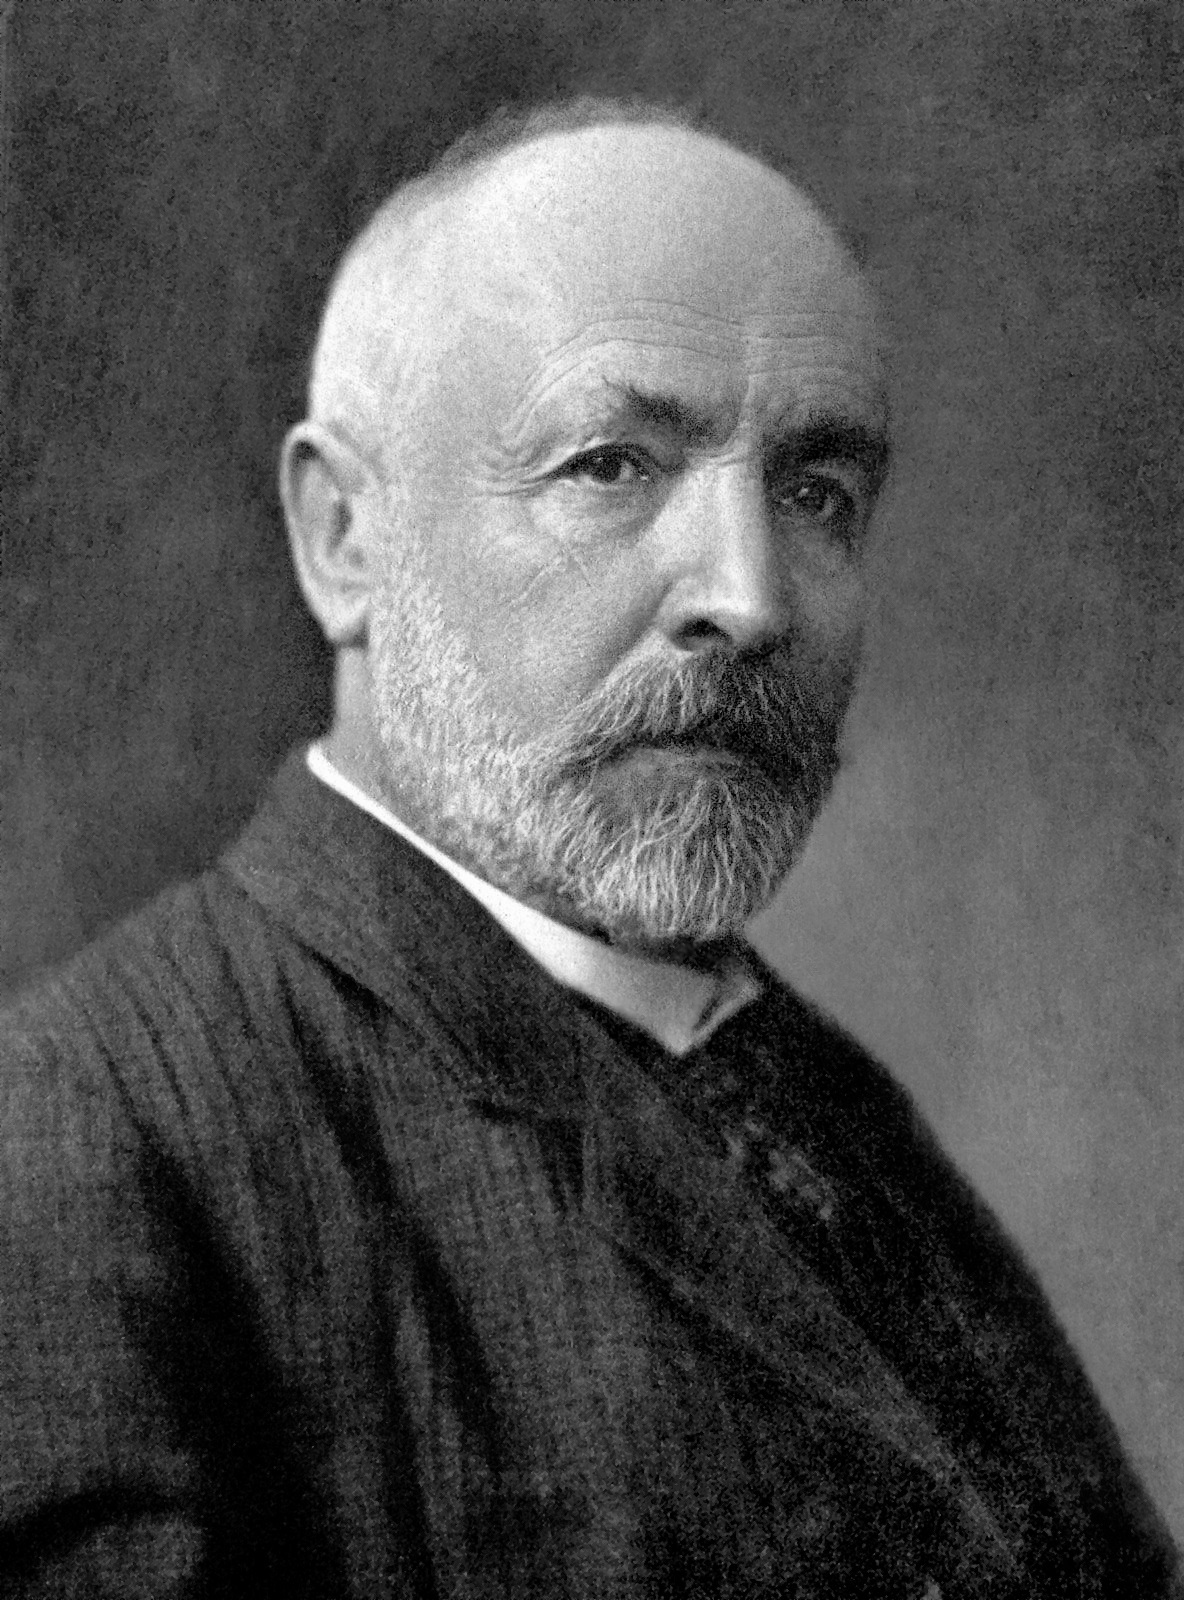
\includegraphics[scale=0.50]{figures/Cantor1.jpg}\\
%  \vspace{-0.8cm}
%  \caption{Georg Cantor.}
%  \label{cantor1}
%\end{figure}



\inic A teoria teve seu início com a publicação em 1874 de um trabalho de Cantor que tratava sobre a comparação de coleções infinitas.\vskip0.3cm

\inic Cantor, nasceu em São Petersburgo (Rússia), filho do comerciante dinamarquês, George Waldemar Cantor, e de uma musicista russa, Maria Anna Böhm. Em 1856 sua família mudou-se para a Alemanha, continuando aí os seus estudos. Estudou no Instituto Federal de Tecnologia de Zurique. Doutorou-se na Universidade de Berlim em 1867.\vskip0.3cm

\inic Desde 1638, com \textbf{Galileu Galilei}, sabe-se que se pode obter uma correspondência 1-1 entre os números inteiros e seus quadrados, o que violava a concepçao euclidiana de que o todo é sempre maior que qualquer uam de suas partes.\vskip0.3cm

\inic Esta aplicação de correspondência 1-1 permitiu a Cantor introduzir um método de diagnalização, que por contradição, permita provar que o conjunto dos números reais não tinha correspondência 1-1 com o conjunto dos números inteiros. Isto, mais tarde, levou ao desenvolvimento do conceito de contínuo por \textbf{Richard Dedekind}. \vskip0.3cm

\inic Em meados de 1892, Cantor, provou que o conjunto dos números racionais $Q$ é (e)numerável, enquanto que o conjunto dos números reais $IR$ é contínuo (logo, maior que o anterior). Já em 1897, Cantor descobriu vários paradoxos suscitados pela teoria dos conjuntos. Foi ele que utilizou pela primeira vez o símbolo ${\displaystyle \mathbb {R}}$ para representar o conjunto dos números reais.\vskip0.3cm


\inic Iniciando com estas descobertas, Cantor acabou desenvolvendo uma \textbf{Teoria dos Conjuntos} abstratos, que constitui-se em uma generalização do conceito de conjunto usada até hoje em vários ramos de pesquisa. \vskip0.3cm


Perseguido e criticado por sua tese, teve a saúde mental comprometida. Tempos depois, seus métodos foram assimilados e se mostraram perfeitamente práticos e úteis. Reconhecido alguns anos depois, foi nomeado membro honorário da \textbf{London Mathematical Society} e homenageado com a medalha da \textbf{Royal Society of London}.\vskip0.3cm

%Perturbado pelas perseguições, morreu aos 72 anos, em uma clínica psiquiátrica na Alemanha.



\section{Conjuntos}

O conceito de conjunto é fundamental não somente no estudo da
Probabilidade e da Estatística, como para a Matemática em geral.
\emph{Qualquer lista ou coleção bem definida de entidades ou
objetos é chamada conjunto}, os objetos que individualmente formam
ou compõem a coleção ou conjunto são chamados \emph{elementos ou
membros}. Em geral, denota-se um conjunto por uma letra maiúscula
($A,B,C,...$) e um elemento do conjunto por letra minúscula
($a,b,c,...$).\vskip0.3cm

\section{Sunconjuntos}

Se todo elemento de um conjunto A é também elemento de um conjunto
B, dizemos que A é subconjunto de B, e escrevemos $A \subset B $
ou $B \supset A$ e lemos "A está contido em B", ou "B contém
A".\vskip0.3cm

Se um elemento $a$ pertence a um conjunto $C$ escrevemos $a \in
C$. Se $a$ não pertence a $C$ escrevemos $a \in C$. Se tanto $a$
como $b$ pertencem a $C$ escrevemos $a,b \in C$. A fim de que um
conjunto seja bem definido, devemos dispor de uma regra que nos
permita dizer se determinado objeto pertence ou não ao
conjunto.\vskip0.3cm

Um conjunto pode ser definido relacionando-se todos os seus
elementos, ou, quando isto não for possível, indicando uma
propriedade que seja válida para todos os elementos do conjunto, e
somente para eles.\vskip0.3cm


Existem três meneiras de descrever que objetos estão contidos no
conjunto A.

\begin{enumerate}
    \item Poderemos fazer uma lista dos elementos de A. Por
    exemplo, $A = \{ 1,2,3,4 \}$ descreve o conjunto formado pelos
    inteiros positivos 1,2,3 e 4.
    \item Poderemos descrever o conjunto A por meio de palavras.
    Por exemplo, poderemos dizer que A é formado de todos os
    números reais entre 0 e 1, inclusive.
    \item Para descrever o conjunto acima poderemos simplesmente
    escrever $A = \{ x|0\leq x \leq 1 \}$; isto é, A é o conjunto
    de todos os x, onde x é um número real entre 0 e 1, inclusive.
\end{enumerate}


\section{Experimentos Aleatórios}

È aquele que repetido em condições idênticas produz geralmente
resultados distintos. Por exemplo jogar uma moeda não viciada,
sabemos que a chance de sair cara é 50\%, mas não conseguimos
prever com exatidão o resultado da jogada, mesmo controlando todas
as circunstâncias relevantes ao experimento.\vskip0.3cm


\textbf{Ex1}: Lançar uma moeda três vezes. \vskip0.3cm

\textbf{Ex2}: Lançar dois dados simultaneamente. \vskip0.3cm

\subsection{Características dos Experimentos Aleatórios}

%Observando-se os experimentos acima pode-se destacar algumas
%características comuns.

\begin{itemize}
    \item Podem ser repetidos indefinidamente sob as mesmas
   condições;
   \item Não se pode adiantar um resultado particular, mas
    pode-se descrever todos os resultados possíveis;
    \item Se repetidos muitas vezes apresentarão uma regularidade
    em termos de frequências de resultados.
\end{itemize}


\section{Fenômenos Aleatórios}

O conceito de fenômeno aleatório é ligeiramente diferente do
conceito de experimento aleatório. Nos experimentos aleatórios
podemos controlar, de certa forma, fatores alheios ao problema os
quais podem influenciar os resultados do experimento, além disso,
podemos "reproduzir" o experimento com certa margem de
liberdade.\vskip0.3cm

Já nos fenômenos aleatórios nós somos meros observadores, os
fenômenos aleatórios tratados pela estatística são aqueles que
possuem "regularidade estatística", isto é, são observáveis e
suceptíveis de repetição.\vskip0.3cm

\textbf{Ex1}: Observar o número de casos de Meningite por mês em
Belém. \vskip0.3cm

\textbf{Ex2}: Observar a quantidade de chuva mensal.\vskip0.3cm



\section{Espaço Amostral ($\Omega$)}

Em um fenômeno aleatório ou probabilístico, isto é, sujeito às
leis do acaso, chamamos \emph{espaço amostral} ou \emph{espaço das
possibilidades} ao conjunto (em geral o mais detalhado possível)
de todos os resultados possíveis de ocorrer. Denota-lo-emos por
$S$ ou $\Omega$.\vskip0.3cm

Por exemplo, se jogarmos um dado vermelho e um dado preto, o
espaço amostral correspondente poderá ser descrito como segue.

$$
S_{1} =
\left[%
\begin{array}{cccccc}
  (1,1) & (2,1) & (3,1) & (4,1) & (5,1) & (6,1) \\
  (1,2) & (2,2) & (3,2) & (4,2) & (5,2) & (6,2) \\
  (1,3) & (2,3) & (3,3) & (4,3) & (5,3) & (6,3) \\
  (1,4) & (2,4) & (3,4) & (4,4) & (5,4) & (6,4) \\
  (1,5) & (2,5) & (3,5) & (4,5) & (5,5) & (6,5) \\
  (1,6) & (2,6) & (3,6) & (4,6) & (5,6) & (6,6) \\
\end{array}%
\right]
$$

onde, digamos, o primeiro número de cada par indica o ponto do
dado branco e o segundo indica o ponto do dado preto.\vskip0.3cm

Entretanto, deve-se notar que, mesmo que os dados fossem
idênticos, o espaço amostral poderia ser considerado análogo pois
a rigor, haveria também 36 resultados possíveis.


$$
S_{2} =
\left[%
\begin{array}{ccccc}
  CCCC  & CCCK  & CCKK  & CKKK  & KKKK \\
        & CCKC  & CKCK  & KCKK  &      \\
        & CKCC  & KCCK  & KKCK  &      \\
        & KCCC  & CKKC  & KKKC  &      \\
        &       & KCKC  &       &      \\
        &       & KKCC  &       &      \\
\end{array}%
\right]
$$

onde C representa cara e K coroa, em cada moeda
lançada.\vskip0.3cm

Com isso, o espaço amostral é dividido em discreto e contínuo.


\subsection{Espaço Amostral Discreto}

Quando as realizações do experimento denotam uma qualidade ou são
resultados de uma contagem, o espaço amostral é dito discreto,
isto é, suceptível de enumeração (finita ou infinita), nesse caso,
cada possível resultado é chamado de evento elementar $\{w_{i}\}$.
$$ \Omega = \{ (w_{1}),(w_{2}),(w_{3}),... \}  $$


\subsection{Espaço Amostral Contínuo}

Quando as realizações do experimento são resultados de uma
mensuração, isto é, os possíveis resultados não são enumeráveis, o
espaço amostral é chamado de contínuo. Neste caso, não faz sentido
falar em eventos elementares e, em geral, os eventos estão
constituídos por intervalos.


\section{Eventos}

Qualquer subconjunto de um espaço amostral será um evento,
definindo um resultado bem determinado. Os eventos podem ser
simples ou compostos, conforme se constituam de um ou mais
resultados de $S$. Designaremos os eventos por letras maiúsculas.


\subsection{Operações com Eventos}

Sejam A e B dois eventos associados a um espaço amostral.

\begin{enumerate}
    \item Se A e B forem eventos, a união entre A e B, denotada por, $A \cup B$ será o evento que
    ocorrerá se, e somente se, A ou B (ou ambos) ocorrerem.
    \item Se A e B forem eventos, a interseção entre A e B, denotada por, $A \cap B$ será o evento que
    ocorrerá se, e somente se, A e B ocorrerem.
    \item Se A for um evento, $\bar{A}$ será o evento complementar que ocorrerá
    se, e somente se, \emph{não ocorrer A}.
    \item Se A e B forem eventos, a diferença de A e B, denotada
    por $A-B$, será o evento que aqueles elementos que estão em A mas
    não estão em B ocorrerá.
    \item Dois eventos, A e B, são \emph{mutuamente excludentes}, se eles
    não puderem ocorrer juntos. Exprimiremos isso escrevendo $A \cap B =
    \phi$, isto é, a interseção de A e B é o \emph{conjunto vazio}.
\end{enumerate}


\newpage
\subsection{Propriedades das Operações}

\begin{enumerate}
    \item Comutativa
$$A \cup B = B \cup A$$
$$A \cap B = B \cup A$$
    \item Associativa
$$A \cup (B \cup C) = (A \cup B)\cup C$$
$$A \cap (B \cap C) = (A \cap B)\cap C$$
    \item Distributiva
$$A \cup (B \cap C) = (A \cup B)\cap (A \cup C)$$
$$A \cap (B \cup C) = (A \cap B)\cup (A \cap C)$$
    \item Leis de Morgan
$$ (A \cup B)^{c}= A^{c} \cap B^{c}$$
$$ (A \cap B)^{c}= A^{c} \cup B^{c}$$
\item Geral
$$ A \cup \phi = A$$
$$ A \cap \phi = \phi$$
$$ \bar{\bar{A}}=A $$
$$ A \cup \bar{A}= \Omega $$
\end{enumerate}















 
\section{Definições de Probabilidade}
 
\inic Historicamente, a probabilidade foi objeto de ampla discussão, tendo sido definida de maneiras diferentes. Assim, houve a definição de probabilidade como sendo o limite da frequencia relativa de ocorrência de um evento quando o número de provas tendia ao infinito. Esta definição, dita \textbf{Fruequêntista}, padecia evidentementa de uma grande limitação.\vskip0.3cm
 
\inic Uma segunda definição, connhecida por \textbf{Clássica}, concebia a probabilidade como sendo quociente do número de casos favoráveis ao evento pelo númeto de casos possíveis, desde que todos igualmente prováveis. Esta definição é hoje considerada uma regra prática para atribuição das probabilidades, quando aplicável.\vskip0.3cm
 
 
\inic Modernamente, se adota a definição \textbf{Axiomática} da probabilidade, proposta em 1933 pelo matemático russo, \textbf{Andrei Nikolaevich Kolmogorov}, segundo a qual a probabilidade obedece as três axiomas.
 
 
\subsection{Definição Frequentista de Probabildade}

\inic Na prática acontece que nem sempre é possível determinar a probabilidade de um evento. Neste caso, é necessário ter um método de aproximação desta probabilidade. Um dos métodos utilizados é a experimentação que objetiva estimar o valor da probabilidade de um evento $A$ com base em valores reais. A probabilidade avaliada através deste processo pe denominado de probabilidade empírica.\vskip0.3cm

\inic Seja $\epsilon$ um experimento e $A$ um evento de um espaço amostral associado ao experimento $E$. Suponha-se que $E$ seja repetido $n$ vezes e seja $m$ o número de vezes que $A$ ocorre nas $n$ repetições de $E$. Então a fraquência relativa do evento $A$, anotada por $f_{r}_{a}$, é o quociente:
 
\begin{equation}
     f_{r_{a}}= \frac{m}{n}
\end{equation}
 
 
%\newpage 
\subsubsection{Propriedades da Frequência Relativa} 

\inic Seja $\epsilon$ um experimento e $A$ e $B$ dois eventos de um espaço amostral associado $S$. Sejam $f_{r}_{a}$ e $f_{r}_{b}$ e as frequências relativas de $A$ e $B$ respectivamente. Então:

\begin{enumerate}
    \item $0 \leqslant f_{r_{a}}  \leqslant 1$, isto é, a frequência ralativa do evento $A$ é um número que varia entre $0$ e $1$.
    \item $f_{r_{a}}= 1$ se e somente se, $A$ ocorre em todas as $n$ repetições de $\epsilon$.
    \item $f_{r_{a}}= 0$ se e somente se, $A$ ocorre em todas as $n$ repetições de $\epsilon$.
    \item $f_{r_{A \cup B}}  = f_{r_{A}} + f_{r_{B}}$ se $A$ e $B$ forem eventos mutuamente excludentes.
\end{enumerate}
 
 
 
 
 
\subsection{Definição Clássica de Probabilidade}
 
\inic Se $E$ um experimento aleatório e $S$ um espaço amostral formado por $n$ resultados igualmente prováveis. Seja $A \subseteq S$ um evento com $m$ elementos. A probabilidade de $A$, anotado por $P(A)$, lê-se $p$ de $A$, é definida como sendo:
  
\begin{equation}
     P(A)= \frac{m}{n}
\end{equation}
  
\inic Isto é, a probabilidade do evento $A$ é o quociente entre o número $m$ de casos favoráveis e o número $n$ de casos possíveis.\vskip0.3cm


\textbf{Exemplo:} Calcular a probabilidade de no lançamento de um
dado equilibrado obter-se:

\begin{enumerate}
    \item Um resultado igual a 4.
    \item Um resultado ímpar.
\end{enumerate}

$$
P(A)= \frac{m}{n}=\frac{1}{6}=16,67\%
$$

$$
P(B)= \frac{m}{n}=\frac{3}{6}=50\%
$$





\inic A definição clássica é dúbia, a já que a idéia de igualmente provável pe a mesma de com probabilidade igual, isto é, a definição é circular, porquer está definindo essencialmente a probabilidade com seus próprios termos. A definição não pode ser aplicada quando o espaço amostral é infinito.


 
\subsection{Definição Axiomática de Probabilidade}
\subsubsection{O Que é Axiomática?}

\inic Em determinadao ponto da evolução de uma teoria de pensamento matemático, torna-se imperioso ordenar, sistemtizar e relacionar todos os conhecimentos entretanto nela reconhecidos, isto é, proceder à sua \textbf{Axiomatização}. 
 
\begin{enumerate}
\item Axiomatizar consiste em escolher algumas afirmações que podem ser feitas sobre os objetos matemáticos em estudo, na área considerada;
\item Delas, por processo dedutivo, obter todas as demais proposições que constituem o corpo de conhecimento da teoria em causa;
\end{enumerate} 

\inic Essas afirmações, das quais deduzimos todas as outras, são os \textbf{Axiomas} e o seu conjunto constitui uma \textbf{Axiomática}.\vskip0.3cm
 

\inic Os Axiomas, além de se basearem numa ceitação por evidência, devem ser:

\begin{enumerate}
    \item Logicamente independente isto é, nenhum deles deve ser passível de se obter dos restantes;
    \item Compatível, isto é, os axiomas não podem, por dedução lógica, conduzir a proposições contraditórias; 
\end{enumerate}
 
 \inic As afirmações que se obtêm dedutivamente a partir dos axiomas, ou de outras já deles obtidas por dedução, chamamos \textbf{Teoremas}.\vskip0.3cm
 
 \inic Em, 1833, \textbf{Kolmogorov} estabeleceu a definição de probabilidade por Axiomatização, na sus obre intitulada \textbf{Foundations of Theory of Probability}. Foi com base nas propriedades das frequências relativas e das operações sobre conjuntos que Kolmogorov concebeu a primeira construção Axiomática Geral para a Teoria das Probabilidades.\vskip0.3cm


\subsubsection{Axiomas de Probabilidade}

\inic Seja $E$ um experimento aleatório com um espaço amostral associado. A cada evento $A \subset B$ associa-se um número real, representado por $P(A)$ e denominado de probabilidade de $A$, que satisfaz as seguintes propriedades(axiomas).

\begin{enumerate}
    \item Se $\phi$ for o conjunto vazio, então
    $P(\phi)=0$.

\textbf{Demostração}: Para qualquer evento $A$, podemos escrever
$A=A\cup \phi$. Uma vez que $A$ e $\phi$ são mutuamente
excludentes, decorre que, $P(A)=P(A\cup \phi)= P(A)+P(\phi)$,
assim, $P(A)- P(A)= P(\phi)= 0$.
    \item Se $\bar{A}$ for o evento complementar de $A$, então
    $P(A)=1-P(\bar{A})$.

\textbf{Demostração}: Podemos escrever $\Omega = A \cup \bar{A}$
e, então, $P(\Omega)= P(A)+ P(\bar{A})$, assim, a $P(\Omega)=1$,
com isso, $1= P(A)+P(\bar{A})$, ou seja, $P(\bar{A})= 1- P(A)$.
    \item Se A e B forem dois eventos \emph{quaisquer}, então $P(A\cup B)=P(A)+P(B)-P(A\cap B)$

\textbf{Demostração}: A idéia desta demostração é decompor $A\cup
B$ e $B$ em dois eventos mutuamente excludentes e, em seguida,
aplicar a propriedade da soma. Desse modo escreveremos,

$$A \cup B= A\cup (B\cap \bar{A})$$
$$B= (A \cap B) \cup (B\cap \bar{A})$$

consequentemente,

$$P(A \cup B)= P(A)+P(B \cap \bar{A})$$
$$ P(B) = P(A \cap B) + P(B \cap \bar{A})$$

Subtraindo a segunda igualdade da primeira, obtém-se

$$ P(A \cup B) - P(B) = P(A)- P(A \cap B)$$
 e daí chega-se ao resultado

$$ P(A \cup B) = P(A)+P(B)- P(A \cap B)$$
    \item Se A, B e C forem três eventos quaisquer, então $P(A \cup B \cup C) = P(A)+P(B)+P(C)-P(A\cap B)-P(A\cap C)-P(B\cap C)+P(A\cap B \cap C)$


\textbf{ \maltese Demostração}: A demostração consiste em escrever
$A \cup B \cup C$ na forma $(A \cup B)\cup C$ e aplicar o
resultado do teorema anterior. Deixa-se a cargo do estudante
completar a demostração.

    \item Se $A \subset B$, então $P(A) < P(B)$
\end{enumerate}

\textbf{Demostração}: Podemos decompor B em dois eventos
mutuamente excludentes, na seguinte forma $B = A \cup (B \cap
\bar{A})$. Consequentemente, $P(B) = P(A)+ P(B \cup \bar{A}) \geq
P(A)$, porque $P(B \cap \bar{A}) \geq 0$.


\subsubsection{Consequências dos Axiomas}

\inic De acordo com os Axiomas, apresentados anteriormente, serão definidos algumas propriedades, como consequências diretas:

\begin{enumerate}
\item Se $\phi$ for o conjunto vazio, então $P(\phi)=0$
\item Se $\bar{A}$ for o evento complementar de $A$, então $P(A)=1-P(A)$
\item Se $A$ e $B$ forem dois eventos quaisquer, então $P(A \bigcup B)= P(A)+P(B)-P(A \bigcap B)$ 
\item Se $A$, $B$ e $C$ forem três eventos quaisquer, então $P(A \bigcup B \bigcup C)= P(A)+P(B)+P(C)- P(A \bigcap B)- P(A \bigcap C)- P(B \bigcap C)+P(A \bigcap B \bigcap C)$
\item Se $A \subset B$, então $P(A) \prec P(B)$
\end{enumerate}



\newpage
\section{Probabilidade Condicional}

Seja A e B dois eventos associados ao experimento $\varepsilon$.
Denotaremos por P(B/A) a probabilidade condicionada do evento B,
Quando A tiver ocorrido.\vskip0.3cm

Sempre que calcularmos P(B/A), estaremos essencialmente calculando
P(B) em relação ao espaço amostral reduzido A, em lugar de fazê-lo
em relação ao espaço amostral original $S$.\vskip0.3cm

Quando calcularmos P(B) estaremos nos perguntando quão provável
será estarmos em B, sabendo que devemos estar em S. È quando
calcularmos P(B/A) estaremos perguntando quão provável será
estarmos em B, sabendo que devemos estar em A. Isto é, o espaço
amostral ficou reduzido de S para A.



\begin{equation}\label{}
    P(B/A) = \frac{P(A \cap B)}{P(A)}, \quad \quad desde \quad que
    \quad P(A)>0.
\end{equation}

\begin{equation}\label{}
    P(A/B) = \frac{P(A \cap B)}{P(B)}, \quad \quad desde \quad que
    \quad P(B)>0.
\end{equation}

È simples verificar as seguintes propriedades de P(B/A) para A
fixado:

\begin{enumerate}
    \item $0 \leq P(B/A) \leq 1$
    \item $P(S/A)=1$
     \item $P(B_{1} \cup B_{2}/A) = P(B_{1}/A)+P(B_{2}/A)$ se os
     eventos $B_{1}$ e $B_{2}$ forem mutuamente execludentes, $B_{1}\cap B_{2}=\emptyset$
     \item $P(B_{1} \cup B_{2} \cup ... / A) =
     P(B_{1}/A)+P(B_{2}/A)+...$ se $B_{i}\cup B_{j}=\phi$ para $i\neq
     j$.
\end{enumerate}



\textbf{Exemplo 1}: Dois Dados equilibrados são lançados,
registrando-se o resultado como ($x_{1},x_{2}$), onde $x_{i}$ é o
resultado do i-ésimo dado, i=1,2. Por isso, o espaço amostral S
pode ser representado pela seguinte lista de 36 resultados
igualmente prováveis.


$$
\Omega =
\left[%
\begin{array}{cccccc}
  (1,1) & (2,1) & (3,1) & (4,1) & (5,1) & (6,1) \\
  (1,2) & (2,2) & (3,2) & (4,2) & (5,2) & (6,2) \\
  (1,3) & (2,3) & (3,3) & (4,3) & (5,3) & (6,3) \\
  (1,4) & (2,4) & (3,4) & (4,4) & (5,4) & (6,4) \\
  (1,5) & (2,5) & (3,5) & (4,5) & (5,5) & (6,5) \\
  (1,6) & (2,6) & (3,6) & (4,6) & (5,6) & (6,6) \\
\end{array}%
\right]
$$

Considere os dois eventos seguintes:\vskip0.3cm

$A=\{(x_{1},x_{2}|x_{1}+x_{2}=10)\}$

$B=\{(x_{1},x_{2}|x_{1}>x_{2})\}$

\vskip0.3cm

Calcular:

\begin{enumerate}
    \item P(B/A)
    \item P(A/B)
\end{enumerate}


$$P(B/A)=\frac{P(A \cap
B)}{P(A)}=\frac{\frac{1}{36}}{\frac{3}{36}} = \frac{1}{3}$$


$$P(A/B)=\frac{P(A \cap
B)}{P(B)}=\frac{\frac{1}{36}}{\frac{15}{36}} = \frac{1}{15}$$

O evento $A \cap B$ ocorre se, e somente se, a soma dos dois dados
for 10 e se o primeiro dado tiver apresentado um valor maior que o
segundo dado.\vskip0.3cm


\textbf{Exemplo 2}: Uma caixa comtém duas moedas. Uma honesta e
outra com 2 caras. Uma moeda é escolhida aleatoriamente,
arremessada e o resultado observado é cara. Qual a probabilidade
de que o outro lado desta moeda escolhida, seja cara?\vskip0.3cm

Considere os seguintes Eventos.\vskip0.3cm

B=\{o resultado é cara\}.

A=\{A moeda é a de 2 caras\}

\vskip0.3cm

Calcular:

\begin{enumerate}
    \item P(A/B)
    \item P(B/A)
\end{enumerate}


$$P(A/B)=\frac{P(A \cap
B)}{P(B)}=\frac{\frac{2}{4}}{\frac{3}{4}} = \frac{2}{3}$$

Das 4 faces que podem ocorrer, 3 são caras, e duas são caras, com
caras no outro lado da moeda de 2 caras.\vskip0.3cm


A maior consequência da definição de probabilidade condicionada
acima, é obtida ao se escrever:


$$
P(A \cap B)= P(B/A)P(A)
$$
 ou equivalentemente,

$$
P(A \cap B)= P(A/B)P(B)
$$

Isto é, algumas vezes mencionado como o \textbf{Teorema da
Multiplicação} de probabilidade. Podemos aplicar esse teorema para
calcular a probabilidade da ocorrência conjunta dos eventos A e B.
\vskip0.3cm

O teorema da multiplicação de probabilidades pode ser generalizado
para mais de dois eventos, da seguinte maneira:

\begin{equation}\label{}
    P[A_{1} \cap A_{2} \cap ... \cap A_{n}]=
    P(A_{1})P(A_{2}/A_{1})P(A_{3}/A_{1},A_{2})...P(A_{n}/A_{1},...A_{n-1})
\end{equation}

Até aqui empregamos o conceito de probabilidade condicionada a fim
de avaliar a probabilidade de ocorrência conjunta de dois eventos.
Poderemos aplicar esse conceito em outra maneira de calcular a
probabilidade de um evento simples A. Necessitaremos da seguinte
definição:\vskip0.3cm


Dizemos que os eventos $B_{1},B_{2},...,B_{k}$ representam uma
\textbf{Partição do Espaço Amostral S}, quando


\begin{enumerate}
    \item $B_{i} \cap B_{j}=\phi$, para todo $i\neq j$
    \item $\bigcup^{k}_{i=1}=S$
    \item $P(B_{i})>0$ para todo $i$
\end{enumerate}

Explicando: Quando o experimento $\varepsilon$ pe realizado
\textbf{um}, \textbf{e somente um}, dos eventos $B_{i}$
ocorre.\vskip0.3cm

\textbf{Exemplo 1}: Na jogada de um dado,
$B_{1}=\{1,2\},B_{2}=\{3,4,5 \}$ e $B_{3}=\{6\}$ representariam
uma partição do espaço amostral, enquanto $C_{1}=\{1,2,3,4\}$ e
$C_{2}=\{4,5,6 \}$ não o representariam.\vskip0.3cm

Consideremos A um evento qualquer referente a S, e
$B_{1},B_{2},...,B_{k}$ uma partição de S. Poderemos escrever

$$
A = (A \cap B_{1}) \cup (A \cap B_{2}) \cup ... \cup (A \cap
B_{k}).
$$

Naturalmente, alguns dos conjuntos $A \cap B_{j}$ poderão ser
vazios, mas isso não invalida essa decomposição de A. O ponto
importante é que todos os eventos $A \cap B_{1},...,A \cap B_{k}$
são dois a dois mutuamente excludentes. Por isso, poderemos
aplicar a propriedade da adiçãos de eventos mutuamente
excludentes, e escrever


$$
P(A)=P(A\cap B_{1})+P(A\cap B_{2})+...+P(A\cap B_{k})
$$

Contudo, cada termo $P(A\cap B_{j})$ pode ser expresso na forma
$P(A/B_{j})P(B_{j})$ e, daí, obteremos o que se denomina o
\textbf{Teorema da Probabilidade Total}:

\begin{equation}\label{}
P(A)=P(A/B_{1})P(B_{1})+P(A/B_{2})P(B_{2})+...+P(A/B_{k})P(B_{k})
\end{equation}

Este resultado representa uma relação extremamente útil, porque
frequentemente, quando P(A) é pedida, pode ser difícil calculá-la
diretamente. No entanto, com a informação adicional de que $B_{j}$
tenha ocorrido, seremos capazes de calcular $P(A/B_{j})$ e, em
seguida, empregar a fórmula acima.


\newpage
\section{Teorema de Bayes}
\subsection{Quem foi Thomas Bayes}

Sir \emph{Thomas Bayes} foi um matemático britânico e um ministro
da igreja presbiteriana que primeiro utilizou a probabilidade
indutivamente e estabeleceu as bases matemáticas para a inferência
probabilística. Ele nasceu em Londres, em 1702, morreu em
Tunbridge Wells em 1761 (tendo vivido apenas 59 anos), e foi
sepultado no cemitério Bunhill Fields em Londres, onde sua tumba
pode ser facilmente encontrada com o mapa fornecido pelo
cemitério.\vskip0.3cm

Seu trabalho com as probabilidades foi reunido em um ensaio
publicado após a sua morte (em 1763) no livro Philosophical
Transactions of the Royal Society of London. O ensaio Essay
Towards Solving a Problem in the Doctrine of Chances relatou,
entre outras importantes descobertas de Bayes, o famoso Teorema de
Bayes.

\subsection{ O Que É o Teorema de Bayes}

O teorema de Bayes é usado na inferência estatística para
atualizar estimativas da probabilidade de que diferentes hipóteses
sejam verdadeiras, baseado nas observações e no conhecimento de
como essas observações se relacionam com as hipóteses.\vskip0.3cm

Este teorema é uma das pedras angulares da estatística das
probabilidades combinadas, e é largamente utilizada em áreas a
primeira vista pouco relacionadas, como Medicina e
Informática.\vskip0.3cm

Na primeira, o paradigma embasado em evidências é todo construído
em cima do teorema de Bayes. Baseado na experiência acumulada de
exames e testes para tentar diagnosticar uma doença, o médico
enquadra seus pacientes e pode estimar qual a probabilidade de que
uma dada doença esteja se manifestando. Ou seja, dada uma
probabilidade inicial (por exemplo, o paciente é fumante) e
aplicado um exame em que, se sabe, há uma probabilidade de
falsos-positivos e falso-negativos (por exemplo, uma biópsia de
pulmão), o médico sabe qual a probabilidade resultante daquele
paciente ter a doença (por exemplo, câncer de pulmão).\vskip0.3cm

Na informática, muitos dos sistemas de classificação automática
são baseados no teorema de Bayes. Inicialmente o sistema é
treinado, aceitando entradas de humanos que dizem que uma dada
entrada pertencem a determinado grupo. Com o tempo, o sistema
acumula um grande banco dessas informações e, aplicando o teorema
de Bayes, consegue estimar a probabilidade de cada novo dado de
pertencer a cada grupo já classificado.\vskip0.3cm


\subsection{Definição}

Seja $B_{1},B_{2},...,B_{k}$ uma partição do espaço amostral S e
seja A um evento associado a S. aplicando-se a definição de
probabilidade condicionada, poderemos escrever


\begin{equation}\label{bayes}
    P(B_{i}/A)=\frac{P(A/B_{i})P(B_{i})}{\sum_{j=1}^{k}P(A/B_{j})P(B_{j})}
\end{equation}


Esse resultado é conhecido como \emph{Teorema de Bayes}. È também
denominado fórmula da probabilidade das causas (ou dos
antededentes). Desde que os $B_{i}$ constituam uma partição do
espaço amostral um, e somente um, dos eventos $B_{i}$ ocorrerá.


\section{Eventos Independentes}

Já consideramos eventos A e B que não podem ocorrer conjuntamente,
isto é, $A\cap B = \phi$. Tais eventos são denominados mutuamente
excludentes, ou eventos incompatíveis. Observamos anteriormente
que se A e B forem mutuamente excludentes, então $PA/B=0$, porque
a ocorrência dada de B impede a ocorrência de A. No outro extremo,
temos a situação já estudada, na qual $B \supset A$ e,
consequentemente, $P(B/A)=1$.\vskip0.3cm

Consideremos $P(A \cap B)$, supondo que as probabilidades
condicionadas sejam iguais às correspondentes probabilidades
absolutas. Teremos:

$$
P(A \cap B)= P(A/B)P(B)=P(A)P(B)
$$

$$
P(A \cap B)= P(B/A)P(A)=P(B)P(A)
$$


Desse modo, desde que nem P(A) nem P(B) sejam iguais a zero,
verificamos que as probabilidades absolutas serão iguais às
probabilidades condicionais se, e somente se, $P(A \cap
B)=P(A)P(B)$. Em consequência, formulamos a seguinte definição, a
qual será também válida quer P(A) ou P(B) seja nulo:\vskip0.3cm

\textbf{Definição:} A e B serão eventos independentes se, e
somente se,

$$
P(A \cap B) = P(A)P(B)
$$


Será importante para nós, estendermos a noção de independência
para mais de dois eventos. Consideremos, inicialmente, três
eventos associados a um experimento, digamos A, B e C. Se A e B, A
e C, B e C forem independentes dois a dois (no sentido acima),
então não se concluirá, em geral, que não exista dependência entre
os três eventos.\vskip0.3cm

\textbf{Definição:} Diremos que os três eventos A, B e C são
mutuamente independentes se, e somente se, todas as condições
seguintes forem válidas:

$$
P(A \cap B)=P(A)P(B)
$$

$$
P(A \cap C)=P(A)P(C)
$$

$$
P(B \cap C)=P(B)P(C)
$$

$$
P(A \cap B \cap C)=P(A)P(B)P(C)
$$


Finalmente, generalizando esta noção para n eventos, na seguinte
definição:\vskip0.3cm



\textbf{Definição:} Os n eventos $A_{1},A_{2},...,A_{n}$ serão
mutuamente independentes se, e somente se, tivermos para
$k=2,3,...,n$:

\begin{equation}\label{}
    P(A_{i_{1}} \cap A_{i_{2}} \cap A_{i_{k}})=
    P(A_{i_{1}})P(A_{i_{2}})...P(A_{i_{k}})
\end{equation}




















\newpage
\section{Principais Distribuições de Probabilidade}
 
 
\inic Uma distribuição de probabilidade é um modelo matemático que relaciona um certo valor da variável aleatória em estudo com a sua probabilidade de ocorrência. De conformidade com a natureza da variável aleatória, a distribuição pode ser classificada em discreta ou contínua.
 
\subsection{Distribuição Binomial}

Os princípios básicos da distribuição binomial foram desenvolvidos pelo matemático suíço durante o século XVII chamado \textbf{Jakob Bernoulli}, que fez muitas contribuições à teoria da probabilidade. Foi o autor do que é geralmente conhecido como o primeiro livro dedicado à probabilidade, publicado em 1713.\vskip0.3cm

Em homenagem a Jakob, os ensaios utilizando probabilidade binomial, na maioria das vezes são denominados \textbf{Ensaios de Bernoulli}, e uma sequência desse tipo de ensaios é denominado de \textbf{Processo de Bernoulli} \vskip0.3cm


A distribuição Binomial dá a probabilidade de deterninado desfecho ocorrer em determinado número de ensaios independentes. \vskip0.3cm


\inic A distribuição Binomial é uma distribuição discreta, cuja função de probabilidade é:
 
\begin{equation}
f(y) = C_{n}^{y}p^{y}q^{n-y}
\end{equation}
 
Sendo: \vskip0.3cm

\begin{itemize}
\item $p$ = probabilidade de realização do contecimento favorável; 
\item  $q$ = probabilidade de ralização do acontecimento contrário;  
\item $y$ = número de vezes que se realiza o acontecimento favorável;  
\item $n$ = número de tentativas; 
\item $C_{n}^{y}$ = números de combinações de n elementos, tomados y a y; 
\end{itemize} 




 
\newpage
\subsection{Distribuição de Poisson}

A distribuição de Poisson tem este nome em homenagem ao metemático, Astrônomo e físico francês \textbf{Simeon Denis Poisson}. Com característica próxima a Binomial, a distribuição de Poisson é uma distribuição descontínua, aplicável quando o resultado é o número de vezes que determinado evento ocorre. \vskip0.3cm

Poisson recebeu dois prêmios importantes da época:

\begin{itemize}
    \item \textbf{Prêmio Lalande} (1810) Membro da Academia Americana de Artes e Ciências;
    \item \textbf{Medalha Copley} (For his work entitled, Nouvelle Theorie de lAction Capillaire., 1832)
\end{itemize}

O Prêmio Lalande foi uma condecoração científica em Astronomia, concedida de 1902 a 1970 pela Académie des Sciences. O prêmio homenageia o astrônomo Jérôme Lalande, estabelecido pelo próprio em 1801. Após 1970 foi combinado com o prêmio da fundação Benjamin Valz, concedido até 1996.\vskip0.3cm


A Medalha Copley é um prêmio no domínio das ciências, sendo
a de maior prestígio atribuída pela \textbf{Royal Society} e, também, a mais antiga. Foi concedida pela primeira vez em 1731.\vskip0.3cm


  
\inic A distribuição de Poisson é adequada para descrever as probabilidades do número de ocorrências num intervalo contínuo (em geral tempo ou espaço). São exemplos de variáveis que podem ter como modelo a distribuição de Poisson:

\begin{enumerate}
    \item Acidentes com automóveis em uma determinada estrada;
    \item Quantidade de pacientes que chegam num pronto socorro durante a madrugada;
    \item  Número de leitos necessários em centro de tratamento intensivo;
    \item  Número de Policiais Militares ou Agentes de Trânsito, necessários em um quadro de distribuição de modo a assegurar a disponibilidade de recursos adequados;
\end{enumerate}


\newpage 
\inic Note que a quantidade de valores possíveis que a variável aleatória pode assumir é infinita, entretanto enumerável. Além disso, observe que a variável aleatória é discreta (número de ocorrências), no entanto a unidade de medida é contínua (tempo, área).\vskip0.3cm

Ainda, as falhas não são contáveis. Por exemplo, não é possível contar os acidentes que não ocorreram em um dia, nem tão pouco a quantidade de pacientes que não chegaram ao pronto socorro na madrugada.
 
 
\begin{equation}
    P\left(X=k\right)= \frac{e^{-\lambda}\lambda^{k}}{k!}
\end{equation}

onde:

\begin{itemize}
\item $e$: é a base do logaritmo natural ou neperiano;
\item $k$: quantidade de ocorrências num intervalo contínuo;
\item $k!$: é o fatorial de $k$; 
\item $\lambda$: é um número real que representa a taxa de ocorrência. Por exemplo, se o evento ocorre a uma média de 4 minutos e estamos interessados no número de eventos que ocorrem num intervalo de 10 minutos, $\lambda={10}/{4}=2.5$
\end{itemize}

  
Além disso, temos que o valor esperado e a variância serão: 

$$
\begin{aligned}
E\left[X\right] =\lambda \\
Var\left(X\right) = \lambda
\end{aligned}
$$
 


\newpage
\subsection{Distribuição Normal}

\inic Quando os valores das observações de uma variável resposta, originados de uma amostra, são agrupados em tabelas de frequências, objetiva-se conhecer a variação e como se processa a distribuição dos dados.\vskip0.3cm 

\inic Existem inúmeros tipos de curvas que podem representar as distribuições. Na maioria das pesquisas biológicas, as observações variam em torno da distribuição normal, a qual é uma distribuição contínua, também conhecida como distribuição de Gauss, Laplace ou Laplace-Gauss. É a mais importante distribuição no campo da Estatística e tem a seguinte função de densidade:


\begin{equation}
f\left(x\right) = \frac{1}{\sqrt{2\pi \sigma^2}}exp \left\{-\frac{1}{2}\left(\frac{x-\mu}{\sigma}\right)^2 \right\},~~~-\infty<x<\infty~~\text{e}~\sigma>0 
 \end{equation}



\newpage
\subsection{Distribuição Qui-Quadrado $\chi^{2}$}

\inic A variável aleatória $\chi^{2}$, denominada quiquadrado com $k$ graus de liberdade, é definida como a soma de k quadrados de normais padronizadas e independentes. 


\newpage
\subsection{Distribuição $t$ de $Student$}
\subsubsection{A Origem da $t$ $student$}

William Sealy Gosset nasceu em 13 de junho de 1876 em Canterbury, Inglaterra, o primeiro de cinco filhos do Coronel Frederic Gosset e Agnes Sealy Vidal. Ele tinha problemas de visão e não conseguia seguir seu pai na Royal Engineers, mas ele era um aluno muito bom e ganhou várias bolsas de estudo.\vskip0.3cm


Ao final do século XIX, a famosa \textbf{Arthur Guinness Son and Company} era a maior cervejaria do mundo, e foi pioneira em diversos esforços para o Controle de Qualidade. Em 1899, um dos contratados para o cargo de químico, recém-formado na Universidade de Oxford, com 23 anos de idade e um currículo que combinava matemática e estatística, foi \textbf{William Sealy Gosset}.\vskip0.3cm

%\begin{figure}[!htb]
%\centering{
% 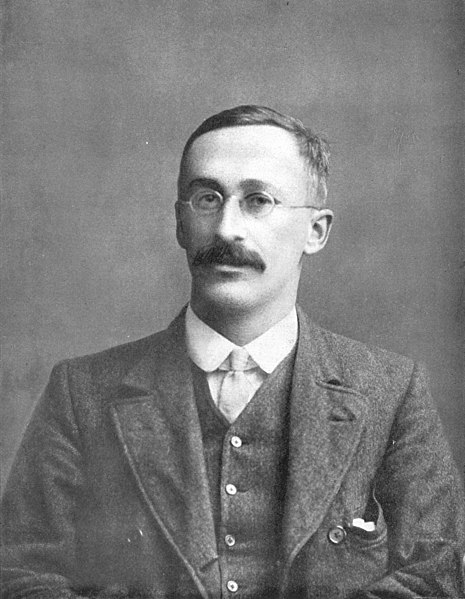
\includegraphics[scale=0.5]{figures/Gosset2.png}\\
%  \vspace{-0.8cm}
%  \caption{William Sealy Gosset, 1908}\label{esquematabela1}}
%\end{figure}


A Guinness era uma empresa de Agro-Química progressista e Gosset iria aplicar os seus conhecimentos de estatística tanto na cervejaria (a destilaria) como nas quintas, para a selecção dos melhores espécimens de cevada.\vskip0.3cm

O trabalho de Gosset na Guinness consistia em medir os inúmeros fatores do processo de produção e ponderar como eles se relacionam aos resultados do produto final. William realizou muitos testes para estimar a duração da cerveja diante das diferentes condições de armazenagem, fabricação e transporte.\vskip0.3cm


Gosset desenvolveu o teste t, distribuição passível de ser tabulada, como um modo barato de monitorar a qualidade da cerveja. Na época, não existia uma teoria para a tomada de decisões com base em pequenas amostras. Por isso, o grande diferencial desse teste é justamente permitir que se façam inferências usando um menor número de elementos. \vskip0.3cm

Um outro funcionário da Guinness tinha já publicado um trabalho que continha alguns segredos da Cervejeira Guinness. Para prevenir fugas de informação e futuras revelações dos "segredos" da marca, a Guinness proibiu que os seus empregados pudessem publicar quaisquer trabalhos independentemente do conteúdo. Isto queria dizer que Gosset não tinha como publicar os trabalhos com o seu nome. Então, usou o pseudonimo $Student$ para as suas publicações evitando ser detectado pela entidade empregadora. \vskip0.3cm

\newpage
Desta forma, o seu feito mais conhecido, é hoje conhecido com a Distribuição t-Student, que noutras circunstâncias seria conhecida como a Distribuição t-Gosset.\vskip0.3cm


Gosset trabalhou na cervejaria em St. James's Gate por 36 anos, antes de se tornar o cervejeiro-chefe de uma nova cervejaria Guinness em Park Royal em Londres.\vskip0.3cm

Em outubro de 2012, uma placa foi inaugurada na Escola Nacional de St Patrick, Blackrock(Irlanda), para homenagear William Sealy Gosset, que morou nas proximidades por 22 anos. \vskip0.3cm

Sir \textbf{Ronald Fisher}, um gigante entre os estatísticos, chamou Gosset de “O Faraday das Estatísticas”, reconhecendo sua capacidade de compreender princípios gerais e aplicá-los a problemas de importância prática.



\subsubsection{A Distribuição $t$ }

Seja a variável aleatória:

\begin{equation}
    t =\frac{\overline{y}-\overline{Y}}{\frac{s(Y)}{\sqrt(n)}}
\end{equation}

Esta variável é conhecida com distribuição $t$ student, com $k=n-1$ graus de liberdade, podendo também ser escrita na forma:

\begin{equation}
    t =\frac{N(0,1)}{\sqrt{\frac{\chi^{2}_{n-1}}{n-1}}}
\end{equation}

O $s(y)$ é considerado o desvio-padrão estimado.\vskip0.3cm

O gráfico da função densidade da variável $t$ de student é simétrico e tem uma forma parecida com a distribuição normal, entretando, menos achatada, com a média zero e variância igual $\frac{k}{(k-2)}$, em que $k>2$ graus de liberdade. A função densidade da variável $t$ é dada pela expressão (2.10). 

\begin{equation}
f\left(t\right)=\frac{1}{\sqrt{k \pi}}\frac{\Gamma\left(\frac{k+1}{2}\right) }{\Gamma \left(\frac{k}{2}\right)}\left(1+\frac{t^2}{k}\right)^{-\left(\frac{\upsilon+1}{2}\right)},~~~-\infty<x<\infty
\end{equation}













\newpage
\subsection{Distribuição F de Snedecor}






A Estatística \textbf{F de Snedecor} é definida como a razão de duas variáveis independentes com distribuição $\chi^{2}$, ou seja:

\begin{equation}
    F_{k,p}=\frac{\frac{\chi^{2}_{k}}{k}}{\frac{\chi^{2}_{p}}{p}}
\end{equation}

O valor $k$ é o número de graus de liberdade do numerador e o $p$ é o número de graus de liberdade do denominador. A função densidade da distribuição F de Snedecor é dada pela Equação (2.9).


 
\setcounter{chapter}{2} \chapter{Principais Métodos de Amostragem}

\section{Introdução}

O objetivo de todo projeto de pesquisa é, a partir do estudo de uma amostra, fazer inferência para uma determinada população. Logo, para que i inferência estatística seja válida, é necessário que a amostra que a amostra seja representativa da população de onde foi retirada, de maneira que os resultados encontrados sejam os mais fidedignos possíveis. (CALLEGARI-JAQUES , 2003). Assim, é necessário que o autor do projeto atente para os fatores importantes, tais como o método de amostragem e o cálculo do amostral, pois, amostras mal selecioandas e de tamanho inadequado, compormetem o resultado da pesquisa, uma vez que não representam fielmente a população (DAWSON, 2003).
\vskip0.3cm

Nesse sentido, é importante realçar que o cálculo do tamanho amostral
tem sido um dos maiores desafios para aqueles que desejam conduzir um experimento científico, pois nem sempre os métodos para esse cálculo se apresentam de maneira simples e compreensíveis, o que traz ansiedade e dúvidas ao pesquisador (BEIGUELMAN, 2002).
\vskip0.3cm

Para Silva (2004) os levantamentos por amostragem, tem com a
finalidade de produzir instantaneos das realidades estudadas, os
levantamentos por amostragem reunem as seguintes caracteristicas
operacionais:

\begin{enumerate}
    \item[{i})] Aplicam-se conjuntos reais e finitos, compostos de
    elementos denominados de população de estudo.
    \item[{ii})] os elementos podem ser seres humanos, animais, árvores,
    fichas, prontuários, domicílios, áreas ou objetos.
    \item[{iii})] As caraterísticas ou atributos são observados em cada
    elemento e posteriormente agregados por meio de medidas
    estatísticas chamadas parâmetros ou valores populacionais.
\vskip0.3cm
    \item[{iv})] Os dados são coletados em amostras das populacões de
    estudo, e as medidas calculadas (estimativas) passam a ser a
    informação disponível para os valores populacionais
    desconhecidos.
\end{enumerate}


De acordo com Silva (2004), os levantamentos pode ter finalidade
\textbf{descritiva}, limitando-se a estimar frequências de
elementos com determinada propriedade ou estimar médias e
variâncias de características quantitativas.\vskip0.3cm

Outros levantamentos, denominados \textbf{analíticos ou
investigaões}, definem grupos de comparação e, além de estimar,
procuram detectar relações entre as características, buscando
aumentar as explicações para o objeto pesquisado (SILVA,
2004).\vskip0.3cm

\inic Existem alguns tipos de levantamentos, técnicas ou métodos
recomendados para a extração de uma amostra, a fim de que esta
possa ser considerada suficientemente representativa da população.
Essas técnicas chamadas de amostragem podem ser classificadas em
duas categorias: as Probabilísticas e Não
Probabilísticas.\vskip0.3cm




A amostragem é dita \textbf{Probabilística ou Casual} quando se
conhece a probabilidade (diferente de zero) que cada elemento da
população tem em fazer parte da amostra. Portanto, para obtenção
de uma amostragem probabilística é necessário que a população seja
finita e que todos os elementos sejam acessíveis. As principais
técnicas de amostragem probabilísticas são: \textbf{amostragem
casual ou aleatória simples}, \textbf{amostragem sistemática},
\textbf{amostragem estratificada} e \textbf{amostragem por
conglomerados} (MATTAR, 2001).\vskip0.3cm

A amostragem é dita \textbf{Não-Probabilística} ou \textbf{Não
Casual} quando nem todos os elementos da população têm
probabilidade conhecida, e diferente de zero, de pertencer à
amostra. Apesar das vantagens do uso da amostragem probabilística,
existem situações onde sua utilização é praticamente impossível.
Isso ocorre principalmente nas situações onde não se tem acesso a
toda população e nos casos em que a população é formada por
material contínuo, tornando impraticável um sorteio rigoroso.
Existem basicamente três tipos de amostragem não-probabilística:
\textbf{amostragem por conveniência}, \textbf{amostragem
intencional} e \textbf{amostragem por quotas} (MATTAR,
2001).\vskip0.3cm


De modo geral as pesquisas utilizam amostras obtidas através de regras probabilísticas. A utilização incorreta da estatística pela amostragem (algumas vezes devido à ingenuidade, porem muitas vezes proposital), mediante a não observância destas regras, pode conduzir a resultados tendenciosos.\vskip0.3cm

\newpage 

Muitas pesquisas partem de amostragem para obter resultados que possam explicar determinados fenômenos. A fim de que uma amostra seja efetivamente representativa da população devem-se adotar técnicas recomendadas para selecionar os elementos que irão compor a amostra, para que não se crie alguma tendenciosidade (o mesmo que viés), que vem a ser uma distorção sistemática entre a medida de uma variável estatística e o valor real da grandeza a estimar, devida a imperfeição ou deformação da amostra que serve de base para a estimativa.\vskip0.3cm


O uso de amostras, substituindo toda a população, em um trabalho de análise estatística se justifica sempre que:
\begin{itemize}
\item Não se tem acesso a todos os elementos da população;
\item O custo de trabalhar com toda a população for muito alto;
\item O tempo para a coleta de dados for um fator relevante;
\item A amostra é a única opção no caso que o estudo exige a destruição ou contaminação dos elementos pesquisados;
\item Quando a população for infinita.
\end{itemize}


O uso de amostras pode proporcionar maior rapidez no trabalho, porém exige determinados cuidados na obtenção das mesmas. Uma amostra de boa qualidade deve ser:

\begin{itemize}
\item Precisa: exatidão dos resultados das medições obtidas na mostra;
\item Eficiente: quando produz resultados de maior precisão ou mesma precisão quando comparado a outro método, porém de menor custo;
\item Correta: ausência de vício ou sem erros sistemáticos.
\end{itemize}



\newpage
\subsection{Fatores que Afetam o Tamanho da Amostra} 
\inic Existem alguns fatores que afetam o tamanho da amostra em projetos de pesquisas científicas nas diversas áreas.

\begin{itemize}
\item \textbf{Objetivo da Amostra}: estudos descritivos costumam exigir amostra com menror número de particpantes;
\item \textbf{Tipo de variável}: as variáveis qualitativas exigem amostras maiores que as variáveis quantitativas, que exigem amostras maiores quanto maior for a variação nos dados amostrais; 
\item \textbf{Delineamento do Estudo}: estudo pareado requer uma amostra com metade do número de sujeitos, quando comparados aos estudos não-pareados;
\item \textbf{Valor Estimado para o Erro Alfa}: corresponde ao erro máximo que o pesquisador aceita cometer ao aplicar o teste estatístico para aceitar ou rejeitar hipótese nula. È o erro máximo que ele aceita para um erro falso-positivo. Na área das ciências da saúde é estipulado em 5\%. Quanto menor o erro alfa estipulado pelo pesquisador, maior será o tamanho estimado para a amostra. 
\item \textbf{Poder do Teste Estatístico}: corresponde a probabilidade de que o estudo detecte uma diferença real entre os grupos estudados. Traduz a probabilidade de o pesquisador cometer um erro falso-positivo. Na área das ciencias sa saude e arbitrado em 80\%, 85\% ou 90\%, que corresponde a um erro beta de 20\%, 15\% e 10\%.Quanto maior o tamanho da amostra, maior será o poder do estudo em detectar uma diferença ou um efeito real;
\item \textbf{O Tamanho da Diferença}: corresponde ao tamanho da verdadeira diferença que se dejesa discriminar como significativa, entre as médias da variável considerada no estudo. pequenas diferenças exigem amostras maiores;
\item \textbf{O Tamanho da População}: para pequenas populações o tamanho da amostra é diretamente proporcional ao tamanho da população. Para grandes populações, o tamanho da amostra não é influenciadao pelo tamanho da população, pois a mesma deverá ser considerada como ilimitada;
\item\textbf{ Dos Recursos e do Tempo Disponível}: é outro fator limitante que, não menos importante, pode influenciar no tamanho da amostra.
\end{itemize}


\subsection{Procedimentos Amostrais Iniciais}

\inic O cálculo do tamanho de uma amostra, impõe ao pesquisador
que ele especifique um valor predefinido para o erro amostral
(margem de erro), o qual deve ser pensado em termos de
probabilidades, pois, mesmo que uma amostra seja sificientemente
grande, ele não garante que suas características sejam exatamente
iguais a da população de onde foi retirada, uma vez que sempre
existe a probabilidade da randomização gerar uma amostra bem
diferente da população. Ou seja, a margem de erro exprime o valor
de quanto o pesquisador admite errar na avaliação dos parametros
estudados (FONTELLES et al, 2009).\vskip0.3cm

Inicia-se com a análise da situação em que não se pode determinar
o tamanho da população (N). Nesse caso, o tamanho mínimo da
amostra aleatória simples pode ser determinado através do cálculo
de $n_{0}$, considerado uma primeira aproximação para o cálculo do
tamanho da amostra, dado por


\begin{equation}\label{nzero}
    n_{o}=\frac{1}{\left(\epsilon_{0}\right)^2}
\end{equation}

Sendo $\epsilon_{0}$ o erro amostral máximo tolerável.\vskip0.3cm

A expressão acima apresentada mantém fixo o nível de confiança de 95\% e a variância populacional no caso de maior heterogeneidade da população, ou seja, quando a proporção do evento na população em estudo é de 0,5. A fixação da proporção populacional do evento em 0,5, deve-se ao fato de ser esta a pior situação possível em termos de variabilidade populacional. \vskip0.3cm

Assim, pode-se considerar que a expressão (2.1) destina-se a três
situações: uma primeira, na qual não se conhece uma estimativa da
proporção do evento na população em estudo, uma vez que qualquer
que seja o valor da proporção, este dá origem a uma variabilidade
menor que aquela vinculada à proporção 0,5. Observa-se que, neste
caso é preciso maior cuidado com a determinação da amostra e,
conseqüentemente, a quantidade de elementos que a
comporão.\vskip0.3cm

Uma segunda situação na qual o valor de uma estimativa preliminar para a proporção do evento estudado é igual a 0,5 e, uma última, na qual o estudo destina-se à estimação da proporção de vários eventos da população, com pelo menos um dos eventos sem presença de uma estimativa anterior de sua proporção na população.\vskip0.3cm


\newpage
A seguir, apresenta-se uma tabela com aplicações da fórmula acima para alguns valores de erro amostral tolerável, a fim de se exemplificar a relação entre $\epsilon_{0}$ e uma primeira estimativa para o tamanho da amostra ($n_{0}$).




\begin{table}[!htb]
    \centering
    {
    \caption{Exemplos de tamanho de amostra ($n_{0}$) em função do erro amostral tolerável, variando de 1 a 5\%}
    \label{amostras}
    \vspace{0.1cm}
\begin{tabular}{c|c}
  \hline\hline
  % after \\: \hline or \cline{col1-col2} \cline{col3-col4} ...
  Erro Amostral $(\varepsilon_{(0)})$   & Tamanho Amostral ($n_{(0)})$ \\
  \hline\hline
  0,010    &  10.000 \\
  0,015    &  4.444 \\
  0,020    &  2.500 \\
  0,025    &  1.600 \\
  0,030    &  1.111 \\
  0,035    &  816 \\
  0,040    &  625 \\
  0,045    &  494 \\
  0,050    &  400 \\
  \hline\hline
\end{tabular}}
\\
\hspace{-1.0cm}
\end{table}

%\newpage

Conforme pode-se observar na tabela 2.1, quanto menor o erro
amostral tolerado pelo pesquisador, maior o tamanho da amostra
necessário para se atendê-lo. Considerando que o erro amostral
tolerável representa o quanto o pesquisador admite errar na
estimação dos parâmetros de interesse, ou seja, especifica o
intervalo em torno do valor que a estatística acusa, dentro do
qual encontra-se o verdadeiro valor do paramêtro que se deseja
estimar, quanto menor o erro amostral tolerado pelo pesquisador,
maior será o tamanho da amostra para que se possa obter essa maior
precisão da estatística.\vskip0.3cm



Assim, por exemplo, se o pesquisador tolerar no máximo um erro de 2\%, i.e., que o verdadeiro valor do parâmetro seja no máximo 2\% menor ou 2\% maior que o valor que a estatística acusa na amostra, ele terá que trabalhar com uma amostra aleatória composta por 2.500 indivíduos da população, ao passo que, se o pesquisador tolerar um erro amostral de 2,5\%, ele terá que trabalhar com uma amostra aleatória composta por 1.600 indivíduos da população e o verdadeiro valor do parâmetro da população estará no intervalo entre 2,5\% a menos até 2,5\% a mais do valor que a estatística acusa na amostra, com 95\% de probabilidde. Portanto, quanto maior a precisão que se deseja associar à estimativa estatística, maior o tamanho amostral necessário para atendê-la.\vskip0.3cm


\newpage
Conhecendo-se o tamanho da população N, pode-se corrigir o cálculo de $n_{0}$, obtido por \ref{nzero}, para se ter o tamanho da amostra aleatória simples, n, através da expressão:


\begin{equation}\label{nzero2}
    n=\frac{\left(N \times n_{0}\right)}{\left(N + n_{0}\right)}
\end{equation}


Para exemplificar, Rocha (2013) fez um levantamento junto a
Delegacia de Crimes contra a Mulher de Macapá (AP) no  período de
agosto de 2011 a junho de 2012, do universo das ocorrências
registradas, há um total de 1.735 de ocorrências consideradas por
aquele órgão estatal como solucionadas. Desse total, 994 são
relativos à violência conjugal distribuídos da seguinte forma: 546
solucionadas, de agosto a dezembro de 2011 e 448 solucionadas, de
janeiro a junho de 2012. Para a realização do estudo optou-se em
retirar uma amostra representativa do total referente à violência
conjugal, por meio das fórmulas demonstradas anteriormente.

\vskip0.3cm


O valor do $\varepsilon_{0}=erro$ a ser adotado será de 5\%.
Portanto, substituindo o valor do erro na expressao 2.1

\begin{equation}\label{nzero}
    n_{o}=\frac{1}{\left(\epsilon_{0}\right)^2}=\frac{1}{\left(0,05
    \right)^2}=400
\end{equation}

Em seguida, substituindo o resultado na formula 2.2,

\begin{equation}\label{nzero2}
    n=\left(\frac{N \times n_{0}}{N + n_{0}}\right)=
    \left(\frac{994 \times 400}{994 + 400}\right)=285
\end{equation}

Assim, faz-se necessário, apenas uma amostra de 285 ocorrências
registradas sobre violência conjungal, sendo esta,
estatísticamente representativa da população de 994.



\newpage
\section{Amostragem Probabilística}
\inic  Os Principais métodos de amostragem probabilísticas são: Aleatória Simples, Sistemática, Estratificada e Conglomerado.

\subsection{Amostragem Aleatória Simples (AAS)}

\inic Este tipo de amostragem também chamada de Simples ao Acaso,
Casual Simples, Elementar ou Randômica. Basei-se num processo
estritamente aleatório, na qual as unidades amostrais são
selecionadas com igual probabilidade $(\frac{1}{N})$, em que N é o
número total de unidades que compõem o espaço amostral, ou seja, a
população amostrada (QUEIROZ, 2012).\vskip0.3cm


A amostragem aleatória simples pode ser feita com reposição (caso em
que cada elementos da população pode entrar mais do que uma vez na
amostra) ou sem reposição (caso em que cada elemento da população
são pode entrar uma vez na amostra).\vskip0.3cm



Na amostra simples ao acaso sem reposição, as unidades são selecionadas independentemente entre si, e o número de amostras possíveis (nap) de tamanho igual a n é dada pela relação:


\begin{equation}\label{nap}
    nap=\mathcal{C}_{N}^{n}=\frac{N!}{n!(N-n)!}=\left(\frac{N}{n}\right)^{-1}
\end{equation}

A amostra simples é um processo congruente, ou seja, quando n=N, as estimativas coincidem com os valores populacionais, recomendada para pequenas àreas com caracteristicas homogêneas com respeito as variáveis de interesse e com fácil estrutura de acessibilidade.

\subsection{Amostragem Estratificada (AE)}

\inic Muitas vezes a população se divide, em sub-populações,
subconjuntos ou estratos, sendo razoável supor que em cada estrato
a variável de interesse (sendo estudada) apresente um
comportamento substancialmente diverso. Por outro lado, pode-se
supor que o comportamento é razoavelmente homogêneo dentro de cada
estrato. Em tais casos, se o sorteio dos elementos da amostra for
realizado sem se levar em consideração a existência dos estratos,
pode acontecer que os diversos estratos não sejam convenientemente
representados na amostra, o que influenciara o resultado pelas
características dos estratos mais favorecidos pelo sorteio.
Evidentemente, a tendência à ocorrência desta influência será
tanto maior quanto menor for o tamanho da amostra. Para evitar
este efeito, pode-se adotar uma amostragem estratificada.\vskip0.3cm

A amostragem estratificada consiste essencialmente em
pré-determinar quantos elementos da amostra serão retirados de
cada estrato. A pré-determinação pode ser feita de várias formas,
sendo as mais comuns chamadas de uniforme (onde se sorteia um
número igual de elementos em cada estrato) e proporcional (onde o
número de elementos sorteados em cada estrato é proporcional ao
número de elementos no estrato).\vskip0.3cm



A amostragem estratificada uniforme será recomendável se os
estratos da população forem pelo menos aproximadamente do mesmo
tamanho. Caso contrario, será preferível a estratificação
proporcional pelo fato de fornecer uma amostra mais representativa
da população.\vskip0.3cm

%\newpage

A estratificação pode levar em conta mais de um critério: por
exemplo, além do estado civil, poderiamos pré-determinar a
estratificação da amostra levando em conta faixas etárias (já que
dispomos de informação detalhada da distribuição dos indivíduos
por faixa etária nos censos de população)\vskip0.3cm

É importante observar, entretanto, que a precisão de uma amostra
não depende de unicamente da dimensão da população, mas também da
respectiva variabilidade. A variabilidade de um estrato é elevada,
quando os seus elementos têm características muito heterogêneas.
Tal situação implica que um estrato com maior variância deverá
levar à seleção de um maior número de unidades na amostra, quando
comparado com um estrato com a mesma dimensão populacional mas
menor variância (maior homogeneidade).\vskip0.3cm

Em resumo, quanto maior for o estrato, maior deve ser a amostra
respectiva. Mas se a variabilidade dentro de um estrato for maior,
maior deverá ser a respectiva sub-amostra. Este método otimiza a
amostra aplicada a um universo estratificado, razão pela qual
também é conhecida como distribuição estratificada
otimizada.\vskip0.3cm




A amostragem estratificada consiste em dividir uma população de
tamanho N e L subpopulações constituídas de
$N_{1},N_{2},\ldots,N_{L}$ unidades, tal que não haja superposição
e, juntas, totalizem a população de tamanho N, ou seja:

\begin{equation}\label{N}
    N=\sum_{h=1}^{L}N_{h}, \ tal \ que \ h=1,2,\ldots,L
\end{equation}


As subpopulações, denominadas estratos, devem ter os valores
$N_{h}$ conhecidos, pois dentro de cada estrato, separadamente,
seleciona-se uma amostra de tamanho $n_{h}$. A grandeza amostral
para a população será igual a $n=n_{1}+n_{2}+\ldots+n_{L}$.
\vskip0.3cm

Assim, para se calcular o tamanho de amostra estratificada
proprocional a cada estrato da população, utiliza-se a seguinte
fórmula (QUEIROZ, 2012),

\begin{equation}\label{amostestra}
n_{h_{i}}= n \times \frac{N_{h_{i}}}{N}
\end{equation}

onde, 

\begin{itemize}
\item $N$ é o número total de unidades em que a população foi dividida;
\item $N_{h}$ é o número de unidades em que o h-ésimo estrato foi dividido;
\item $n$ é o número de unidades de amostra a serem medidas considerando todos os estratos;
\item $n_{h}$ é o número de unidades de amostra a serem medidas no h-ésimo estrato;
\item $W_{h}={\frac{N_{h}}{N}}$ é o peso do h-ésimo estrato;
\item $\frac{n_{h}}{N_{h}}$= fator de amostragem no h-ésimo estrato; 
\item $L$ é o número de estratos;
\end{itemize}

Em relação à aplicação da amostragem, uma população pode ser classificada como finita ou infinita. Determinadas populações finitas podem ser consideradas infinitas desde que o tamanho da amostra seja no máximo 5\% da áream ou seja:

\begin{itemize}
    \item 1) Se $\frac{(N_{h}-n_{h})}{N_{h}} \geqslant 0,95$, a população é definida como Infinita; 
    \item 2) Para $\frac{((N_{h}-n_{h}))}{N_{h}} < 0,95$, a população é definida como Finita;
    \item O termo $\frac{((N_{h}-n_{h}))}{N_{h}}$ é denominado correção para populaão Finita.
\end{itemize}













%\newpage

A amostragem estratificada é recomendadável para o estudo de
populações que apresentem heterogeneidade entre as subpopulações
com referência à variável de interesse. Neste caso, a
estratificação pode propiciar um aumento no grau de precisão,
pois, torna possivel subdividir uma população heterogênea em
estratos que, individualmente, sejam homogêneos, resultando ganho
em eficiência e diminuição dos custos.\vskip0.3cm


A determinação dos estratos é feita em função das características
peculiares da população, onde, em muitos casos, os estratos já
estão fisicamente definidos. Por outro lado, existem casos em que
a delimitação dos estratos só é possível através de levantamentos
específicos.\vskip0.3cm


O processo para obter os estratos denomina-se estratificação e a
amostra é dita estratificada. Denomina-se amostra acidental
estratificada quando são selecionadas amostras inteiramente ao
acaso nos estratos.\vskip0.3cm

Conforme Cochran (1965), existem diversos critérios para se
utilizar o método de amostragem estratificada. Os principais são
os seguintes:


\begin{enumerate}
  \item[{1)}] A estratificação ideal é aquela realizada segundo a magnitude do valor da variável de interesse,
  obtendo-se gnho de precisão quando houver variação sensível entre os estratos definidos;
  \item[{2)}] Razões administrativas podem direcionar para a utilização de estratificação, visando
  principalmente caracterizar peculiaridades locais e regionais;
\end{enumerate}


\newpage
\textbf{Exemplo de Amostragem Estratificada}
\vskip0.3cm

Castro et al (2016), realizou um estudo com informações retiradas de processos
judiciais de homens e mulheres adultos, que foram acusados de praticar agressão
sexual contra as crianças e adolescentes entre os anos de 2012 a 2014, período esse
escolhido por concentrar um maior número de processos no Sistema de Gestão de
Processos Judiciais - LIBRA, do Tribunal de Justiça do Estado do Pará. Nos quais,
foram escolhidos três municípios como população alvo, que supriam e respondiam aos objetivos do trabalho.

\begin{table}[!htb]
    \centering
    {
    \caption{Número de Processos judiciais sobre práticas de agressão sexual com criancas e
adolescentes julgados pelo TJE em três municípios Paraenses no período de 2012 a 2014.}
    \label{amostras estratificada}
    \vspace{0.1cm}
\begin{tabular}{c|c|c}
  \hline\hline
  Municípios   & Nº de Processos &  Percentual \\
  \hline\hline
   Abaetetuba  & 47              & 6.69        \\
   Belém       & 555             & 82,22       \\
   Parauapebas & 73              & 10,81       \\
  \hline\hline
\end{tabular}}
\\
\hspace{-1.0cm}
\end{table}

De acordo com a tabela 2.3, vericou-se que, as maiorias dos processos estão
concentradas no município de Belém (82,2\%), 10,8\% em Parauapebas e apenas 6,9\%
em Abaetetuba. Porém, os processos não são digitalizados, contendo muitas páginas
cada um, e tendo que ser acessado em horários restritos no TJE, não podendo fazer
cópias dos mesmos. Dificultando, assim, o trabalho de catalogação de todos os 675
processos de agressão sexual, levando-se em conta, as caracteríssticas dos autores, das
vitimas e a tipificação das agressões. Com isso, devido a diversos fatores, optou-se
em trabalhar com uma amostra estatisticamente representativa da população em estudo.
\vskip0.3cm

Assim, para a um erro amostral de 5\%, tem-se a primeira estimativa para o tamanho da amostra em estudo dos processo judiciais.

\begin{equation}\label{nzero}
    n_{o}= \left[\frac{1}{\left(\epsilon_{0}\right)^2}\right] = \left[\frac{1}{\left(0,05
    \right)^2}\right]=400
\end{equation}

Em seguida, substituindo o resultado na formula 2.2,

\begin{equation}\label{nzero2}
    n=\left(\frac{N \times n_{0}}{N + n_{0}}\right)=
    \left(\frac{675 \times 400}{675 + 400}\right)=251
\end{equation}

Assim, faz-se necessário, apenas um amostra de 251 processos judiciais sobre
agressão sexual, sendo esta, estatiscamente representativa da população de 675.
\vskip0.3cm

Contudo, a população alvo está dividida em três municípios com quantidades
de processos diferentes em cada. Havendo a necessidade de levantar o tamanho da
amostra levando-se em conta que, o número de elementos sorteados em cada estrato
é proporcional ao numero de elementos no estrato, chamado Método de Amostragem
Estratificada Proporcional.
\vskip0.3cm

Assim, para se calcular o tamanho de amostra estratificada proprocional a cada
município (estrato) da população, utiliza-se a fórmula abaixo,

%\begin{equation}
%\end{equation}

$$
n_{h_{1}}= n \times  \left(\frac{N_{h1}}{N} \right)= 251 \times \frac{47}{675}= 18
$$

$$ 	n_{h_{2}}= n \times \left(\frac{N_{h1}}{N} \right)=251 \times \frac{555}{675}= 206 $$

$$ 	n_{h_{3}}= n \times \left(\frac{N_{h1}}{N} \right)= 251 \times \frac{73}{675}= 27 $$

$$ n = \left( n_{h_{1}} + n_{h_{2}} + n_{h_{3}}\right) = 18+206+27 = 251
$$




\subsection{Amostragem Sistemática (AS)}


A amostragem sistemática consiste em sortear uma unidade da população e, a partir dela, para constituir
uma amostra de tamanho n, selecionar as unidades que ocupam de forma sequencial as suposições multiplas
de um determinado valor $k=\frac{N}{n}$ pré-estabelecido, onde N é o número de unidades total da população (QUEIROZ, 2012).\vskip0.3cm

No processo de amostragem sistemática a primeira unidade é escolhida ao acaso e as demais, a partir da inicial, selecionadas de modo sistemático a intervalos iguais e definidas, até atingir o tamanho da amostra desejada. O intervalo é estabelecido pela razão entre o tamanho da população e o tamanho da amostran (AYRES, 2010).\vskip0.3cm

De acordo com Loetsch et al (1973) a amostragem sistemática consiste em selecionar unidade de amostras a partir
de um esquema rígido e preestabelecido de sistematização segundo uma distribuição espacial equitativa ou mecânica, com os propósitos de cobrir a população em toda a sua extensão, e obter um modelo sistemático simples e uniforme.\vskip0.3cm


A amostragem sistemática apresenta uma diferença marcante com relação a amostragem aleatória simples, no que tange
ao número de amostras possíveis. Sendo recomendada para utilização quando os elementos da população encontram-se
ordenados (MARQUES, 2002).\vskip0.3cm



Seja uma população composta por N unidades, e n represente o tamanho da amostra, sendo $N=kn$. Se a amostragem for sistematica, o número de amostras possíveis é igual a $k=\frac{N}{n}$, enquanto que, em se tratando de uma amostra simples ao acaso sem reposição, o número de amostras possíveis (nap) será de acordo com a equação \ref{nap}. Então, teoricamente, uma amostra sistemática não pode ser analisada como se fosse uma amostra aleatória simples. \vskip0.3cm



De forma geral, na amostragem sistematica, utiliza-se a ordenação
natural dos elementos da população (prontuários, casas, ordem de
nascimento, etc), considerando N o tamanho da população e n o
tamanho da amostra, calcular o intervalo de amostragem, ou o pulo
sistematico, chamado k, por meio da formula $k=\frac{N}{n}$, senfo
k um numero inteiro mais proximo.\vskip0.3cm

Posteriormente, sorteia-se um numero entre um e k, chamado i,
sendo $0 < i \leq k$. Esse numero i será o primeiro elemento da
amostra. O segundo elemento da amostra será $i+k$, o terceiro
elemento será $i+2k$, e assim sucessivamente, de forma sistematica
até $i+(n-1)k$, ou seja, até completar o valor de n.

\vskip0.3cm


\textbf{Vantagens da Amostragem Sistemática}
\vskip0.3cm

A amostragem sistemática, quando comparada com a amostra simples, apresenta algumas vantagens, entre as quais:



\begin{enumerate}
  \item[{a)}] A seleção das unidades amostrais, na amostragem sistemática, é mais fácil e mais rápida, economizando tempo na obtenção dos dados de campo;
  \item[{b)}] A organização, a supervisão e a checagem (remedição) de algumas unidades de amostras se tornam operacioanalmente mais fáceis;
  \item[{c)}] O tamanho da população não precisa, necessariamente, ser conhecido;
  \item[{d)}] A redução de custo ocasionados pelo encaminhamento entre as unidades de amostras;
  \item[{e)}] As unidades se distribuem mais uniformemte na população, originalmente uma maior representatividade, tornando-se eficiente quando existe qualquer tendência ou concentração de certas características;
  \item[{f)}] È possível mapear a população;
  \item[{g)}] A amostragem sistemática pode ser associada  a amostragem por conglomerado;
\end{enumerate}

%\newpage


\textbf{Desvantagens da Amostragem Sistemática}
\vskip0.3cm


\begin{enumerate}
  \item[{a)}] A grande desvantagem da amostra sistematica ocorre
  quando a população apresenta dados com características \textbf{cíclicas}
  \textbf{ou periódicas}, pois corre-se o risco da amostragem refletir
  homogeneidade numa condição sabidamente heterogênea;
  \item[{b)}] Escolhe-se somente uma unidade de amostra simples, as demais não são independentes (estatisticamente, cada unidade não corresponde a um grau de liberdade). Assim, a variância da amostra e a da média não podem ser calculados através dos estimadores usuais;
  \item[{c)}] Escolhidos as amostras sistematicamente, todas as outras uniadades de amostra que não a integram têm probabilidade igual a zero de serem eleitas, enquanto as que integram-na possuem probabilidade 1 de seleção, ou seja, muitas unidades de amostras são, nesse caso, rejeitadas;
\end{enumerate}

\textbf{Exemplo de Amostragem Sistemática}
\vskip0.3cm

Retomando-se o exemplo de Castro et al (2016), ao qual calculou-se o tamanho da
amostra estratificada porporcional por municípios, ao fazer o levantamento deparou-se com elementos da população em forma de pilhas de processos judiciais ordenados
e sequenciais. Havendo assim, a necessidade de se aplicar o Método de Amostragem
Sistemático para se mapear a população de forma fácil e rápida.


\begin{table}[!htb]
    \centering
    {
    \caption{Número de Processos judiciais sobre práticas de agressão sexual com criancas e
adolescentes julgados pelo TJE em três municípios Paraenses no período de 2012 a 2014.}
    \label{amostras estratificada}
    \vspace{0.1cm}
\begin{tabular}{c|c|c}
  \hline\hline
  Municípios   & Nº de Processos &  Percentual \\
  \hline\hline
   Abaetetuba  & $N_{h1}=47$     & $n_{h1}= 6.69$        \\
   Belém       & $N_{h2}=555$    & $n_{h2}= 82,22$       \\
   Parauapebas & $N_{h3}=73$     & $n_{h3}= 10,81$       \\
   \hline\hline 
   Total       & $N_{Total}=675$ & $n_{total}=251$ \\ 
  \hline\hline
\end{tabular}}
\\
\hspace{-1.0cm}
\end{table}


%\vskip0.3cm

A amostragem sistemática consiste em selecionar unidade de amostras a partir
de um esquema rígido e preestabelecido de sistematização segundo uma distribuição
espacial equitativa ou mecânica, com os propósitos de cobrir a população em toda
a sua extensão, e obter um modelo sistemático simples e uniforme.
\vskip0.3cm

De forma geral, na amostragem sistemática, utiliza-se a ordenação natural dos
elementos da população (nesse caso os processos judiciais de agressores sexuais),
considerando N o tamanho da população (675) e n o tamanho da amostra (251),
calcular o intervalo de amostragem, ou o pulo sistemático, chamado k, por meio da
fórmula abaixo,

\begin{equation}
K=\frac{N}{n}=\frac{675}{251}=3
\end{equation}

Posteriormente, sorteia-se um número entre 1 e k=3, chamado i, sendo que esse
número i serão o primeiro elemento da amostra. O segundo elemento da amostra será
(i+3), o terceiro elemento será (i+2)3, e assim sucessivamente, de forma sistemática
até i(n-1)3, ou seja, ate completar o valor de amostra n=251.\vskip0.3cm

Assim calcula-se o k, verifica-se que sorteando um número entre 1 e k=3, tem-se
o número i=2, assim, a amostra ficará da seguinte maneira:



\begin{table}[!htb]
    \centering
    {
    \caption{Amostragem sistemática sobre práticas de agressão sexual com crianças e adolescentes julgados pelo TJE em três municípios Paraenses no período de 2012 a 2014.}
    \label{amostras estratificada}
    \vspace{0.1cm}
\begin{tabular}{c|c|c|c|c|c|c|c|c|c}
  \hline\hline
   2  & 5  & 7  & 10 & 13 & 15 & 18 & 21 & 24 & 26 \\
   29 & 32 & 34 & 37 & 40 & 42 & 45 & 48 & 50 & 53 \\
   56 & 58 & 61 & 64 & 67 & ... & ... & ... & ... & 674 \\
  \hline\hline
\end{tabular}}
\\
\hspace{-1.0cm}
\end{table}




\newpage
\subsection{Amostragem Por Conglomerados (AC) ou Clusters}

\inic Apesar de a amostragem estratificada apresentar resultados
satisfatórios, a sua implementação é dificultada pela falta
de informações sobre a população para fazer a estratificação.\vskip0.3cm

Para poder contornar esse problema, pode-se trabalhar com o
esquema de levantamento chamado amostragem por conglomerados.\vskip0.3cm

Os conglomerados são definidos em razão da experiência
do gestor ou do pesquisador. Geralmente, podemos definir os
conglomerados por fatores geográficos, como bairros e quarteirões.
A utilização da amostragem por conglomerados possibilita uma
redução significativa do custo no processo de amostragem.\vskip0.3cm

A amostragem por conglomerados ou também chamada de clusters, é usada quando a população
pode ser dividida em subpopulações heterogêneas.\vskip0.3cm

Uma amostragem por conglomerado é indicada quando:


\begin{itemize}
  \item Não se possui uma lista contendo todos os nomes dos elementos da população;
  \item Existe grande heterogeneidade entre os elementos da população-alvo;
  \item É preciso fazer entrevistas ou observações em grandes áreas geográficas;
\end{itemize}


As unidades de amostragem ou grupos podem ser espaçadas como ocorre naturalmente em unidades geográficas ou físicas (por exemplo, estados, delegações ou distritos); em base  a uma organização como escolas, grau escolar; ou serviço telefônico, tais como códigos de área ou alterar o código de área do serviço dos números de telefone.\vskip0.3cm

Duas grandes dimensões são utilizadas para classificar os diferentes tipos de amostragem por conglomerados. Uma baseia-se no número de fases do projeto da amostra, e o outra na representação proporcional de grupos na amostra total..\vskip0.3cm


\section{Amostragem Não Probabilística}


Os métodos de amostragem não probabilística, dirigido ou também chamados de não aleatória, são métodos ad-hoc de caracter pragmático ou intuitivo e são largamente utilizados, pois possibilitam um
estudo mais rápido e com menores custos.




\subsection{Amostragem por Conveniência ou Acidental}


\inic A amostragem por conveniência é adequada e freqüentemente utilizada para geração de idéias em pesquisas exploratórias, servindo como base para geração de hipóteses e insights.\vskip0.3cm



A amostra por conveniência é empregada quando se deseja obter informações de maneira rápida e barata. Segundo diversos autores, uma vez que esse procedimento consiste em simplesmente contatar unidades convenientes da amostragem, é possível recrutar respondentes tais como estudantes em sala de aula, mulheres no shopping, alguns amigos e vizinhos, entre outros. Este método também pode ser empregado em pré-testes de questionários.\vskip0.3cm


As amostras por conveniência são o tipo de amostragem menos confiável pois o pesquisador seleciona a amostra conforme sua conveniência, havendo pouco rigor na seleção, onde não há como saber se todas as pessoas incluídas na amostra são representativas da população.\vskip0.3cm



Nos casos de amostragem por conveniência, a diferença entre os valores da população de interesse e os valores da amostra é desconhecida, em termos de tamanho e de direção. Não é possível mensurar os erros desta amostragem e não é possível fazer nenhuma declaração definitiva ou conclusiva sobre os resultados obtidos, não sendo recomendadas para estudos causais e descritivos.




\subsection{Amostragem Intencional ou por Julgamento}

A seleção de amostras intencionais ou por julgamento são realizadas de acordo com o julgamento do pesquisador, sendo comum a escolha de experts (profissionais especializados) usados para escolher emementos "típicos" e "representativos" para uma amostra.
\vskip0.3cm


A abordagem da amostragem por julgamento pode ser útil quando é necessário incluir um pequeno número de unidades na amostra. O método de julgamento é muito utilizado para a escolha de uma localidade "representativa" de um país na qual serão realizadas outras pesquisas, sendo algumas vezes até preferida em relação à seleção de uma localidade por métodos aleatórios.

\newpage 
\subsection{Amostragem por Quotas ou Proporcional}


A amostra por quotas constitui um tipo especial de amostra intencional, em que o pesquisador procura obter uma amostra que seja similar à população sob algum aspecto.\vskip0.3cm

A seleção de amostra por quotas é a forma mais usual de amostragem não probabilística. Neste caso, são consideradas várias características da população como gênero, idade, raça e renda familiar, incluindo proporções similares de pessoas com as mesmas características.\vskip0.3cm


A idéia de amostragem por quotas sugere que se as pessoas são representativas em termos de características, elas também poderão ser representativas em termos da informação procurada pela pesquisa. Depois de serem identificadas as proporções de cada tipo a ser incluído na amostra, o pesquisador estabelece um número ou quota de pessoas que possuem as características determinadas e que serão contatadas pela pesquisa. O entrevistador recebe instruções para continuar a amostragem até que a quota necessária tenha sido atingida em cada estrato.\vskip0.3cm


Uma pesquisa com amostragem por quotas poderá ser utilizado e trazer bons resultados quando as características relevantes para controle e delineamento da amostra forem conhecidas, estiverem disponíveis ao pesquisador, estiverem relacionadas ao objeto de estudo e se constituírem em poucas categorias.

\setcounter{chapter}{3} \chapter{Representação Tabular de Dados}
\section{Tabelas Estatísticas}

\inic Uma vez concluída a coleta e a ordenação dos dados de uma pesquisa, deve-se apresentá-los de tal forma que o leitor consiga identificar, rapidamente, uma série de informações, para tal, costuma-se utilizar inicialmente de uma tabela ou um quadro.\vskip0.3cm

\inic A representação tabular e uma apresentação numérica dos dados. Consiste em dispor os dados em linhas e colunas distribuídos de modo ordenado, segundo algumas regras práticas adotadas pelos diversos sistemas estatísticos. As regras que prevalecem no Brasil foram fixadas pelo Conselho Nacional de Estatística.\vskip0.3cm

\inic Uma tabela é um conjunto de dados estatísticos associados a um fenômeno, dispostos numa ordem de classificação, numa organização racional e prática de apresentação. A tabela resume ou sintetiza os dados, fornecendo o máximo de informação num mínimo de espaço.\vskip0.3cm

\inic Tabela é a forma não discursiva de apresentação de informações, representadas por dados numéricos e codificações, dispostos em uma ordem determinada, segundo as variáveis analisadas de um fenômeno.

\section{Por que Tabelas são Importantes}

\inic Boas tabelas são parte integrante do seu pacote, seja um comunicado de imprensa, um artigo analítico ou um trabalho de pesquisa. O uso eficaz de tabelas ajuda a minimizar o número de valores de dados em seu texto. Também elimina a necessidade de discutir variáveis ​​menos significativas que não são essenciais para o enredo.\vskip0.3cm

As tabelas devem ser independentes, sejam elas publicadas em um relatório, artigo, publicação ou página da web. Cada tabela deve conter metadados suficientes, para permitir que ela seja copiada e colada em outro documento e ainda faça sentido.\vskip0.3cm

Se você garantir que suas tabelas possam ser independentes, é mais provável que elas sejam compreendidas corretamente, dentro ou fora de seu contexto original.

\subsection{Elementos Básicos na Construção Tabular}

\inic Para a construção de uma série ou tabela estatística para que ela seja considerada dentro das normas de exposição. Estes elementos e regras são comuns a todas as tabelas. No Brasil, a apresentação tabular é regida pelas Normas de Apresentação Tabular do IBGE (1993) e NBR 14724 (ABNT, 2014).\vskip0.3cm


Os elementos básicos que constituem uma tabela são:

\begin{enumerate}
  \item \textbf{Número}: é utilizado para identificar a tabela no texto, onde as mesmas são numeradas a partir do número 1, como por exemplo: TABELA 1, TABELA 2, TABELA 3, etc, ou levando-se em consideração o capitulo do texto, como por exemplo, TABELA 1.1, TABELA 1.2, etc, para o capítulo 1, e, TABELA 2.1, TABELA 2.2 para o capítulo 2, e assim, sucessivamente.
  \item \textbf{Título}: Existem alguns mitos sobre o título de uma tabela, alguns autores relatam que, não existe título muito grande. Porém, no Brasil, basta seguir as regras definidas pelo (IBGE, 1993). Assim, o Título é uma designação que se coloca acima da tabela, ele deve ser preciso,
  indicando a natureza, local e época do evento, ou seja, explica o que a tabela contém e todo título deve responder as seguintes questões.

\begin{itemize}
  \item \textbf{O que $?$}  (Referente ao assunto a ser representado (\textbf{Fato}));
  \item \textbf{Como $?$}  (Referente as variáveis escolhidas para análise do fato (\textbf{Tipo}));
   \item \textbf{Onde $?$}   (Relativo ao lugar ou espaço geográfico onde ocorreu o fenômeno (\textbf{Local}));
    \item \textbf{Quando $?$} (Correspondente a época em que se verificou o fenômeno (\textbf{Tempo})).
\end{itemize}

O título deve ser escrito após o número da tabela, devendo ser separado do número por espaço, hífen e espaço, em letra maiúscula como o número. O título da tabela deve fornecer uma descrição clara e precisa dos dados, que seja curto e conciso e evite o uso de verbos.
\newpage
  \item \textbf{Cabeçalho}: parte superior da tabela (primeira linha) na qual é designada à natureza do conteúdo que especifica cada coluna. O cabeçalho pode ter um ou mais níveis. No primeiro nível o cabeçalho deve ser escrito preferencialmente em letras maiúsculas, enquanto que nos demais níveis somente a primeira letra deve ser maiúscula, sendo centralizado em cada coluna.
  \item \textbf{Corpo}: conjunto ou parte da tabela composta por linhas e colunas que contém as informações necessárias, formado pelo cabeçalho, coluna indicadora e numérica, onde o encontro ou cruzamento de uma linha e uma coluna é denominado casa, casela ou célula, sendo utilizado para observar as variáveis em esudo. 
  \item \textbf{Linhas}: Via de regra em pesquisas científicas, na linha são inseridos as respostas de uma pessoa, e nas colunas as variáveis ou características do evento. A linha é a parte do corpo da tabela que contém uma seqüência horizontal de informações.
  \item \textbf{Colunas}: A coluna é a parte do corpo que contém uma seqüência vertical de informações.
  \item \textbf{Casa ou Célula}: È o cruzamento de uma linha com a coluna, onde são indicados os dados e informações, sendo um espaço destinado a um só número.
  \item \textbf{Coluna Indicadora}: coluna que contém as discriminações correspondentes aos valores distribuídos pelas colunas numéricas, ou seja, é a primeira coluna que especifica o conteúdo de cada linha, devendo somente a primeira letra ser maiúscula, exceto quando se utilizarem de expressões que totalizam os dados como TOTAL, sendo alinhada a esquerda. Normalmente, se utilizam as categorias ou subcategorias das variáveis.
  \item \textbf{Rodapé}: É o espaço aproveitado em seguida ao fecho da tabela, reservado a observações pertinentes, onde são colocadas às notas de natureza informativa (fonte, notas, legendas, chamadas, etc).
  \item \textbf{Fonte}: refere-se à indicação das entidades ou órgãos responsável pela organização, origem, elaboração ou fornecimento dos dados expostos na tabela. A palavra fonte deve ser escrita em maiúscula seguida de dois pontos e espaço, seguindo o nome da fonte, sendo permitido o uso de siglas em letras maiúsculas. Deve ficar no rodapé da tabela. 
  \item \textbf{Notas}: São informações de natureza geral (indicados por algarismos romanos), onde o uso de notas, quando necessário, é destinado a esclarecimento (de forma geral ou específica) do conteúdo ou para indicar a metodologia utilizada na coleta dos dados. A palavra nota deve ser escrita em maiúscula seguida de dois pontos, no mesmo padrão do título, estando logo abaixo da fonte. Cada nota deve ser indicada em linha própria, podendo ou não ser numerada ou identificada por símbolos gráficos; As chamadas notas específicas servem para esclarecer minúcias em relação às casas, colunas ou linhas. São indicadas em algarismos arábicos ou símbolos gráficos;
  \item \textbf{Chamadas}: São informações de natureza específica (indicados por algarismos arábicos), colocados acima
  e à direita da coluna indicadora, nas demais colunas acima e a esquerda.
  Em suma, é um símbolo remessivo atribuído a algum elemento de uma tabela
  que necessita de uma nota específica.
\end{enumerate}


\begin{figure}[!htb]
\centering{
  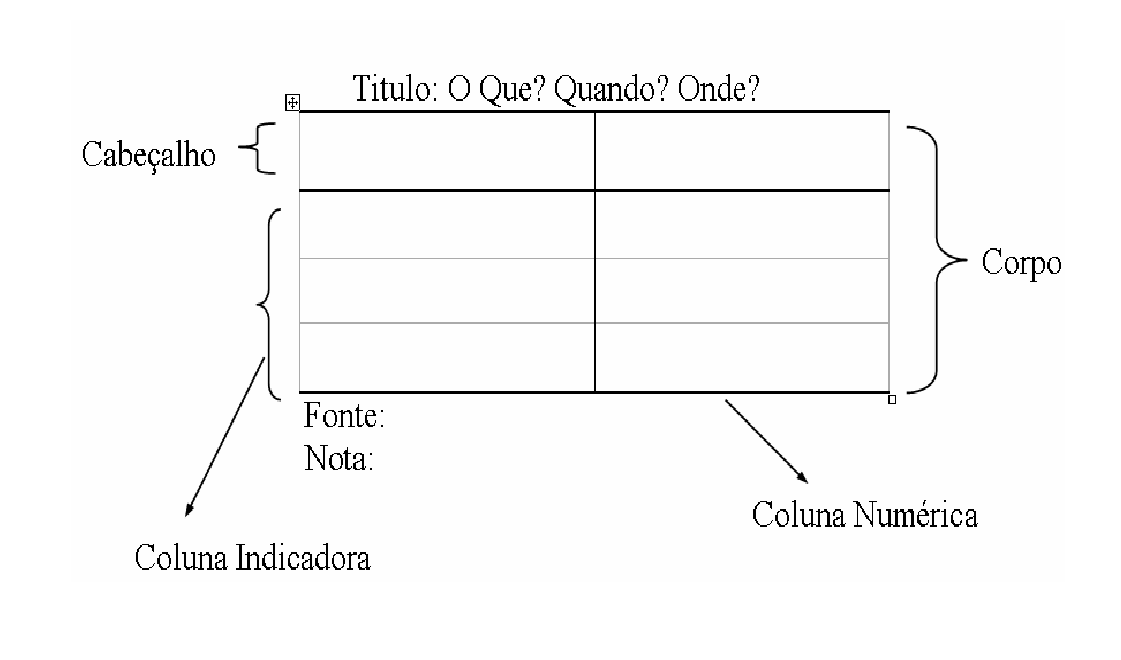
\includegraphics[scale=0.80]{figures/tab1.eps}\\
  \vspace{-0.8cm}
  \caption{Esquema Geral Sobre a Construção de uma
  Tabela conforme a NBR 14724 da ABNT de 2004.}\label{esquematabela1}}
\end{figure}




\newpage
Os valores dos dados devem ser definidos para que as informações principais possam ser extraídas facilmente. Os usuários podem achar mais fácil verificar colunas ou linhas, dependendo da sua mensagem. Você deve considerar isso ao decidir se deseja apresentar sua Tabela na orientação retrato ou paisagem. Linhas ou sombreamentos sutis também podem ser usados para incentivar os usuários a ler horizontalmente, bem como verticalmente. O espaçamento e o sombreamento podem alterar a maneira como uma tabela é lida \vskip0.3cm



Segue um exemplo com dados reais referentes a População Estimada Total do Estado do Pará, para ilustrar o esquema geral sobre uma construção tabular simples, conforme a figura \ref{esquematabela1}.



\begin{table}[!htb]
    \centering
    {
    \caption{\textbf{O Que}:(População Estimada Total) \textbf{De Onde}: (do Estado do Pará e Regiões de Integração), \textbf{Quando}: (2021).}
    \label{amostras estratificada}
    \vspace{0.1cm}
\begin{tabular}{l|c}
  \hline\hline
  \textbf{Cabeçalho}: Estado/Região de Integração   & População Estimada Total \\
  \hline\hline
   \textbf{Pará}                  & 8.8811.659   \\
   Araguaia                       &   583.777    \\
   Baixo Amazonas                 &   750.258    \\
   Carajás                        &   707.165    \\
   Guajará                        & 2.269.233    \\ 
   Guamá                          & 706.880      \\
   Lago de Tucuruí                & 436.351      \\
   Marajó                         & 610.972      \\
   Rio Caeté                      & 532.257      \\
   Rio Capim                      & 711.361      \\
   Tapajós**                      & 257.035      \\
   Tocantins                      & 856.496      \\
   Xingu                          & 389.874      \\
   \hline\hline
\end{tabular}}
\\
\hspace{-6.6cm}
\textbf{Fonte}: MS/DATASUS, 2022. \\
\hspace{-6.5cm}
\textbf{Elaboração}: FAPESPA, 2022. \\
\hspace{-1.0cm}
\textbf{Nota}: (**) População Judicial de Jacareacanga: 41.487 Habitantes.
\end{table}








\newpage
\subsection{Quadros Estatístico}

\inic Os quadros são definidos como arranjo predominante de palavras dispostas em linhas e colunas, com ou sem indicação de dados numéricos. È formado por linhas horizontais e verticais, sendo, portanto "fechado", e normalmente, é usado para apresentar dados secundários.\vskip0.3cm 

\inic Diferenciam-se das tabelas por apresentarem um teor esquemático e descritivo, e não estatístico. A apresentação dos quadros é semelhante à das tabelas, exceto pela colocação dos traços verticais em suas laterais e na separação das casas. Um quadro normalmente apresenta resultados qualitativos (textos). Pode usar espaçamento e fontes de letras com tamanhos menores que o do texto (não precisa seguir o mesmo padrão).   

\begin{quadro}[h!tp]
    \centering
    \caption{Equema geral sobre a construção um Quadro conforme as normas do IBGE de 1993}
    \begin{tabular}{|c|c|}
    \hline
    Cabeçalho  & Coluna indicadora   \\    
    \hline
           &           \\
           &              \\
           &              \\
           &              \\
           &              \\
           &              \\
           &              \\
  \hline
    \end{tabular}
\end{quadro}


%\newpage

\inic Quando um relatório técnico possui tabelas  e Quadros, é necessário inserir uma Lista de Tabelas e Quadros de forma separada.


\newpage
\subsection{Regras para Construção Tabular}

\inic As normas adotadas neste livro, que fixam conceitos e procedimentos aplicáveis a elaboração de tabelas de dados numéricos, de modo a garantir a clareza das informações são apresentadas a seguir (IBGE, 1993)


\begin{enumerate}
\item Quanto a apresentação as tabelas podem ser intercaladas no texto, e imediatamente após o trecho que são citados pela primeira vez, de maneira que sua visualização tenha sentido normal de leitura;  
\item Toda tabela deve ter significado próprio, ou seja, suficientemente completa para ser entendida, dispensando consultas ao texto; 
\item Recomenda-se que uma tabela seja elabora
de forma a ser apresentada em uma única página.
\item Toda tabela contenha somente os dados necessários ao seu entendimento;
\item Inclua os dados logicamente ordenados e apresente dados, unidades e símbolos consistentes com o texto;
\item As tabelas podem ser apresentadas em anexo quando a quantidade de tabelas for grande ou quando ocupar mais de uma página, o que dificultaria a leitura do texto; 
\item Durante a representação em tabelas não se deve ter repetidos seus dados em gráficos ou figuras. Optar por um deles, sem perder de vista o que se quer comunicar, se os valores exatos ou aspecto visual, evitando assim, uma ambiguidade de informações;
\item Deve ter numeração independente e consecutiva; 
\item As tabelas devem ser colocadas em posição vertical para facilitar a leitura das informações, caso a tabela ultrapasse as margens, é necessário \textbf{Rotacionar a Tabela}. Lembrando que, na maioria dos relatórios, quando a tabela ultrapassa as margens, os autores diminuem a fonte para caber em mesma página, cometendo um erro gráfico e estético comum; 
\item Caso a tabela não couber em uma folha,
continuará na folha seguinte e, nesse caso, não é delimitada por
um traço horizontal na parte inferior, sendo o titulo e o
cabeçalho repetido na folha seguinte; 
\item Recomenda-se não
delimitar (fechar) por traços verticais, os extremos da tabela, à
direita e a esquerda, pois, assim, a mesma se torna um quadro;
\item As tabelas, excluídos os títulos, serão delimitadas, no alto e em baixo, por traços horizontais grosso preferencialmente;
\item Devem ser alinhadas de acordo com as margens do texto. O espaço entre as tabelas e texto deve ser de duas entrelinhas;
\item Usa-se um traço horizontal (-) hífen quando o dado for nulo, inexisti o fenômeno; 
\item Usa-se (...) reticência quando não se dispuser dos dados,
embora ele possa ser quantificado; 
\item Usa-se zero (0) quando o
valor é muito pequeno para ser expresso pela unidade utilizada.
\item Caso os dados sejam secundários, as fontes são obrigatórias.
\item Devem preferencialmente ser apresentadas no mesmo tipo e tamanho de letras adotados no texto ou reduzidas até um limite que não prejudique a sua leitura. Nunca em tamanho maior que o texto;
\item Não utilizar mais casas decimais do que o necessário para
não mascarar as comparações de interesse. 
\item Proponha um título
autoexplicativo e inclua as unidades de medidas. O título deve
dizer o que representam os números do corpo da tabela e, em geral,
não deve conter informações que possam ser obtidas diretamente dos
rótulos de linhas e colunas. 
\item Colocar os totais de linhas
e/ou colunas para facilitar as comparações. 
\item Ordene colunas
e/ou linhas quando possível. Se não houver impedimentos, ordene-as
segundo os valores, crescentes ou decrescentes. 
\item Tente trocar
de orientação (linhas por colunas) para melhorar a apresentação,
pois, é mais fácil fazer comparações ao longo das linhas do que
das colunas. 
\item Altere a disposição e o espaçamento das linhas
e colunas para facilitar a leitura. 
\item Não analise a tabela
descrevendo-a, mas sim, comentando as principais tendências
sugeridas pelos dados. 
\item È facultativo o emprego de traços
verticais para separação das colunas no corpo da tabela. 
\item
Quando uma tabela, por exessiva altura, tiver de ocupar mais de
uma página, 
\textbf{Não} deve ser delimitada na parte inferior,
repetindo-se o cabeçalho na página seguinte. Neste Caso, deve-se
usar, no alto no cabeçalho ou dentro da coluna indicadora a
designação continua ou conclusão, conforme o caso. 
\item Quando
uma tabela ocupar páginas confrontantes todas as linhas devem ser
numeradas na primeira e na ultima coluna. 
\item Quando não for
conveniente a apresentação de uma tabela em páginas confrontantes,
deverá a mesma ser dividida em duas ou mais. 
\item Se o disposto
no item anterior se tornar impraticável, por serem as colunas
insuscetíveis de agrupamento, deve-se desmenbrar a tabela em
seções, estas dispostas umas abaixo das outras e separadas por um traço horizontal duplo. 
\item Quando uma tabela tiver poucas
colunas e muitas linhas, poderá ser disposta em duas ou mais
partes, lado a lado, separando-se as partes por um traço vertical
duplo.
\item As expressões que totalizam os dados devem ser destacadas em negrito ou letras maiúsculas. Ex: Total, Subtotal, TOTAL;
\item Nenhuma casa da tabela deve ficar em branco, apresentando sempre um número ou sinal.
\item Deve ser evitado o uso de siglas e abreviaturas que não sejam de uso corrente; quando necessárias devem ser grafadas por extenso como nota na tabela;
\item O cabeçalho deve ser centralizado na coluna, com a letra inicial da primeira palavra maiúscula. O uso de outras letras maiúsculas deve respeitar as regras gramaticais do idioma. É facultativo grafar o cabeçalho em negrito, desde que seja mantida uniformidade em todas as tabelas.
\item A indicação de número no cabeçalho deve ser feita pela letra N, em maiúscula, já convencionado na literatura internacional. A indicação do número relativo deve ser feita pelo seu respectivo símbolo.
\end{enumerate}




%%%%%%%%%%%%%%%%%%%%%%%%% TABELA  %%%%%%%%%%%%%%%%%%%%%%%%%%%%%%%%%%%%%%%%%%%%%%%%%%%


\begin{sidewaystable}
\centering
    {
\caption{Exemplo de Tabela Rotacionada devido a Ultrapassagem da Margem (Item 9) , referente a Frota de Veículos Registrados em alguns Municípios Paraenses em setembro de 2022.}
\label{tabelarotacionada}
    \vspace{0.2cm}
\begin{tabular}{l|c|c|c|c|c|c|c|c}
\hline
Municípios & Automóvel & Motocicleta & Caminhonete  & Camioneta & Caminhão  & ônibus & Trator & Total \\
\hline\hline
Belém      & 220.492  & 127.747      & 27.092       & 17.397    & 9.087     & 3.877  & 1.249  & 5.587 \\
Marabá     & 26.941   & 56.931       & 9.091        & 2.100  & 3.686     & 771      & 649    & 425    \\
Santarém   & 29.295   & 44.002       & 7.674        & 2.680  & 3.042     & 770      & 169    & 1.170  \\ 
Ananindeua & 57.418   & 41.666       & 6.966        & 3.429  & 4.494     & 1.601    & 904    & 749    \\  
Itaituba   & 5.798    & 24.724       & 2.976        & 432    & 1.100     & 145      & 99     & 179    \\  
Redenção   & 10.172   & 35.873       & 4.569        & 353    & 1.771     & 175      & 208    & 257    \\
Castanhal  & 19.899   & 36.172       & 4.240        & 998    & 2.860     & 441      & 537    & 302     \\
Tucuruí    & 7.112    & 17.799       & 2.072        & 447    & 915       & 209      & 92     & 141    \\
Altamira   & 10.693   & 37.980       & 4.795        & 752    & 2.032     & 689      & 95     & 331    \\
\hline
  Total    & 387.820  & 383.294      & 69.475      & 28.588 & 27.997    & 8.678    & 4.002  & 9.141   \\
\hline\hline 
\end{tabular}} 
\begin{flushleft}
Fonte: DETRAN-PA, 2022. 
\end{flushleft}
\end{sidewaystable}
%%%%%%%%%%%%%%%%%%%%%%%%%%%%%%%%%%%%%%%%%%%%%%%%%%%%%%%%%%%%%%%%%%%%%%%%%%%%%%%%%%%%%%%%%%%%%%




\newpage
\begin{table}[!htb]
    \centering
    {
    \caption{Exemplo de Tabela (item 10), Produto Interno Bruto a Preços Correntes(Mil Reais), Pará e Municípios - 2016 a 2019.}  Continua...
    \label{item 10 regras1}
    \vspace{0.1cm}
\begin{tabular}{l|c|c|c|c}
  \hline\hline
  Estado/Município        &     2016    &      2017   &    2018     &     2019     \\
  \hline\hline
   \textbf{Pará}          & 138.107.514 & 155.232.404 & 161.349.602 & 178.376.984  \\
   Abaetetuba             & 1.246.639   & 1.337.353   & 1.413.517   & 1.494.985    \\
   Abel Figueiredo        &   76.699    &   80.633    &   82.186    &   85.169     \\
   Acará                  &   789.271   &   932.175   &  913.952    & 757.480      \\
   Afuá                   &             &             &             &              \\ 
   Agua Azul do Norte     &             &             &             &              \\
   Alenquer               &             &             &             &              \\
   Almeirim               &             &             &             &              \\
   Altamira               &             &             &             &              \\
   Anajás                 &             &             &             &              \\
   Ananindeua             &             &             &             &               \\
   Anapu                  &             &             &             &               \\
   Augusto Corrêa         &             &             &             &               \\
   Aurora do Pará         &             &             &             &    \\
   Aveiro                 &             &             &             &    \\
   Bagre                  &             &             &             &    \\
   Baião                  &             &             &             &    \\
   Bannach                &             &             &             &    \\
   Barcarena              &             &             &             &    \\
   Belém                  &             &             &             &    \\
   Belterra               &             &             &             &    \\
   Benevides              &             &             &             &    \\
   Bom Jesus do Tocantins &             &             &             &    \\
   Bonito                 &             &             &             &    \\
   Bragança               &             &             &             &    \\
   Brasil Novo            &             &             &             &    \\
   Brejo Grande Araguaia  &             &             &             &    \\
   Breu Branco            &             &             &             &    \\
   Breves                 &             &             &             &    \\
   Bujaru                 &             &             &             &    \\
   Cachoeira do Arari     &             &             &             &    \\
   Cachoeira do Piriá     &             &             &             &    \\
\end{tabular}}
\end{table}



\newpage
\begin{table}[!htb]
    \centering
    {
    \caption{Exemplo de Tabela (item 10), Produto Interno Bruto a Preços Correntes(Mil Reais), Pará e Municípios - 2016 a 2019.}  Continuação...
    \label{item 10 regras2}
    \vspace{0.1cm}
\begin{tabular}{l|c|c|c|c}
  \hline\hline
  Estado/Município        &    2016    &    2017   &    2018   &  2019     \\
  \hline\hline
   Cametá                 &  1.138.431 & 1.183.561 & 1.131.454 & 1.150.930      \\
   Canãa dos Carajás      &             &             &             &        \\
   Capanema               &             &             &             &       \\
   Capitão Poço           &             &             &             &              \\ 
   Castanhal              &             &             &             &              \\
   Chaves                 &             &             &             &              \\
   Colares                &             &             &             &              \\
   Conceição ao Araguaia  &             &             &             &              \\
   Concórdia do Pará      &             &             &             &              \\
   Cumaru do Norte        &             &             &             &               \\
   Curionópolis           &             &             &             &               \\
   Curralinho             &             &             &             &               \\
   Curuça                 &             &             &             &    \\
   Dom Eliseu             &             &             &             &    \\
   Elddorado Carajás      &             &             &             &    \\
   Faro                   &             &             &             &    \\
   Floresta  Araguaia     &             &             &             &    \\
   Garrafão do Norte      &             &             &             &    \\
   Goianésia do Pará      &             &             &             &    \\
   Gurupá                 &             &             &             &    \\
   Iguarapé-Açú           &             &             &             &    \\
   Iguarapé-Miri          &             &             &             &    \\
   Inhangapi              &             &             &             &    \\
   Ipixuna do Pará        &             &             &             &    \\
   Irituia                &             &             &             &    \\
   Itaituba               &             &             &             &    \\
   Itupiranga             &             &             &             &    \\
   Jacareacanga           &             &             &             &    \\
   Jacundá                &             &             &             &    \\
   Juruti                 &             &             &             &    \\
   Limoeiro do Ajuru      &             &             &             &    \\
\end{tabular}}
\end{table}





\newpage
\begin{table}[!htb]
    \centering
    {
    \caption{Exemplo de Tabela (item 10), Produto Interno Bruto a Preços Correntes(Mil Reais), Pará e Municípios - 2016 a 2019.}  Continuação...
    \label{item 10 regras3}
    \vspace{0.1cm}
\begin{tabular}{l|c|c|c|c}
  \hline\hline
  Estado/Município        &    2016    &    2017    &  2018      &  2019     \\
  \hline\hline
   Mãe do Rio             &  283.984   &  293.012   &  292.918   & 292.628    \\
   Magalhães Barata       &  64.732    &  75.316    &  81.723    & 74.304    \\
   Marabá                 &  7.487.235 &  8.599.354 &  8.779.878 & 11.417.650 \\
   Maracanã               &             &             &             &              \\ 
   Marapanim              &             &             &             &              \\
   Marituba               &             &             &             &              \\
   Medicilândia           &             &             &             &              \\
   Melgaço                &             &             &             &              \\
   Mocajuba               &             &             &             &              \\
   Moju                   &             &             &             &               \\
   Mojuí dos Campos       &             &             &             &               \\
   Monte Alegre           &             &             &             &               \\
   Muaná                  &             &             &             &    \\
   Nova Esperança Piriá   &             &             &             &    \\
   Nova Ipixuna           &             &             &             &    \\
   Nova Timboteua         &             &             &             &   \\
   Novo Progresso         &             &             &             &    \\
   Novo Repartimento      &             &             &             &    \\
   Òbidos                 &             &             &             &    \\
   Oeiras do Pará         &             &             &             &    \\
   Oriximiná              &             &             &             &    \\
   Ourém                  &             &             &             &    \\
   Ourilândia do Norte    &             &             &             &    \\
   Pacajá                 &             &             &             &    \\
   Palestina do Pará      &             &             &             &    \\
   Paragominas            &             &             &             &    \\
   Parauapebas            &             &             &             &    \\
   Pau D'arco             &             &             &             &    \\
   Peixe-Boi              &             &             &             &    \\
   Piçarra                &             &             &             &    \\
   Placas                 &             &             &             &    \\
\end{tabular}}
\end{table}


\newpage
\begin{table}[!htb]
    \centering
    {
    \caption{Exemplo de Tabela (item 10), Produto Interno Bruto a Preços Correntes(Mil Reais), Pará e Municípios - 2016 a 2019.}  Continuação...
    \label{item 10 regras4}
    \vspace{0.1cm}
\begin{tabular}{l|c|c|c|c}
  \hline\hline
  Estado/Município          &    2016   &    2017 &  2018   &  2019   \\
  \hline\hline
   Ponta de Pedras          &  208.199  & 212.571 & 212.006 & 222.251 \\
   Portel                   &      &      &      &     \\
   Porto de Moz             &      &      &      &  \\
   Prainha                  &             &             &             &              \\ 
   Primavera                &             &             &             &              \\
   Quatipuru                &             &             &             &              \\
   Redenção                 &             &             &             &              \\
   Rio Maria                &             &             &             &              \\
   Rondon do Pará           &             &             &             &              \\
   Rurópolis                &             &             &             &               \\
   Salinópolis              &             &             &             &               \\
   Salvaterra               &             &             &             &               \\
   Santa Bárbara            &             &             &             &    \\
   Santa Cruz do Arari      &             &             &             &    \\
   Santa Isabel do Pará     &             &             &             &    \\
   Santa Luzia do Pará      &             &             &             &   \\
   Santa Maria das Barreira &             &             &             &    \\
   Santa Maria do Pará      &             &             &             &    \\
   Santana do Araguaia      &             &             &             &    \\
   Santarém                 &             &             &             &    \\
   Santarém Novo            &             &             &             &    \\
   Santo Antônio do Tauá    &             &             &             &    \\
   São Caetano de Odivelas  &             &             &             &    \\
   São Domingos do Araguaia &             &             &             &    \\
   São Domingos do Capim    &             &             &             &    \\
   São Félix do Xingu       &             &             &             &    \\
   São Francisco do Pará    &             &             &             &    \\
   São Geraldo do Araguaia  &             &             &             &    \\
   São João da Ponta        &             &             &             &    \\
   São João de Pirabas      &             &             &             &    \\
   São João do Araguaia     &             &             &             &    \\
\end{tabular}}
\end{table}





\newpage
\begin{table}[!htb]
    \centering
    {
    \caption{Exemplo de Tabela (item 10), Produto Interno Bruto a Preços Correntes(Mil Reais), Pará e Municípios - 2016 a 2019.}  Conclusão...
    \label{item 10 regras5}
\begin{tabular}{l|c|c|c|c}
  \hline\hline
  Estado/Município            &    2016    &  2017   &  2018       &  2019    \\
  \hline\hline
   São Sebastião da Boa Vista &  176.914   &  206.893  & 209.187   & 205.087  \\
   Sapucaia                   &  96.808    & 108.012   & 99.547    & 106.318  \\
   Senador JOsé Porfírio      &  119.237   & 126.968   & 135.520   & 163.414  \\ 
   Soure                      &  179.866   & 175.016   & 188.033   & 197.890  \\
   Tailândia                  & 874.419    & 846.793   & 897.544   & 951.254  \\
   Terra Alta                 &  68.169    & 71.819    & 70.380    & 71.606  \\
   Terra Santa                &  458.707   & 527.426   & 510.355   & 464.655 \\
   Tomé-Açú                   &  643.689   & 639.412   & 667.658   & 713.215 \\
   Tracuateua                 &  231.943   & 248.331   & 215.620   & 232.494 \\
   Trairão                    &  310.251   & 329.448   & 294.076   & 286.791 \\
   Tucumã                     &  717.362   & 757.450     & 778.560   & 827.871 \\
   Tucuruí                    &  4.356.154 & 6.461.838   & 7.481.522 & 5.318.264 \\
   Ulianópolis                &  1.305.409 & 1.245.238   & 1.330,085 & 1.590.909 \\
   Uruará                     &  504.096   & 511.969     & 545.493   & 610.827  \\
   Vigia                      &  365.883   & 373.305     & 382.251   & 388.468 \\
   Viseu                      &  664.390   & 613.446     & 486.515   &  491.156 \\
   Vitória do Xingu           & 966.759    &  3.088.937  & 4.375.685 &  4.051.017  \\
   Xinguara                   & 1.157.432  & 1.218.114   & 1.226.364 & 1.294.077 \\
   \hline\hline
\end{tabular}}
\\
\hspace{-6.6cm}
\textbf{Fonte}: IBGE/FAPESPA, 2019. \\
\hspace{-6.5cm}
\textbf{Elaboração}: FAPESPA, 2020.
\end{table}

Toda tabela que ultrapassar as dimensões da página no sentido vertical, conforme exemplo da Tabela \ref{item 10 regras1}, deve obedecer as seguinte regras:

\begin{itemize}
\item [a)] Cada página deve ter o conteúdo do topo e o
Cabeçalho da tabela ou o Cabeçalho da parte;
\item [b)] Cada página deve ter uma das seguintes indicações:
\textbf{Continua} para a primeira, \textbf{Conclusão} para a última e \textbf{Continuação} para as demais;
\item [c)] Cada página deve ter Colunas Indicadoras e seus
respectivos Cabeçalhos;
\item [d)] O traço horizontal da moldura que· separa o rodapé deve ser apresentado somente em cada página que contenha a última linha da tabela;
\item [e)] O conteúdo do rodapé só deve ser apresentado na página de conclusão.
\end{itemize}










\newpage
\section{Séries Estatísticas}

\inic Uma série estatística é um conjunto ou coleção de dados ordenados segundo uma característica comum, as quais servirão posteriormente para se fazer análises e inferências. Resumidamente, uma série é um conjunto de números associados a fenômenos dispostos em correspondência com critério de modalidade. Ou seja, uma série é uma forma de organização mais completa e requer certas regras de construção.\vskip0.3cm


\inic As séries estatísticas em geral são de natureza quantitativa sendo expressas em tabelas ou matrizes operacionais, nas quais os dados são distribuídos de maneira organizada através de textos e números e de acordo com um caráter que é passível de variação (CARVALHO e ARAUJO, 2008).\vskip0.3cm

Pode-se dizer que toda série é uma tabela, mas nem toda tabela é
uma série, pois esta exige homogeneidade, classificação, critérios
de modalidade, segundo: \textbf{Espécie}, \textbf{Local} ou
\textbf{Época}. \vskip0.3cm

As séries podem ser classificadas em \textbf{simples} ou \textbf{conjugadas}. As séries simples são aquelas que apresentam variação em apenas uma das modalidades (espécie, local e tempo). São tabelas com apenas uma entrada e possuem apenas duas colunas. As séries conjugadas apresentam variação em duas ou mais modalidades, ou seja, são tabelas com duas ou mais entradas.\vskip0.3cm

As séries também são divididas em:


\begin{itemize}
  \item \textbf{Séries Homógradas} : aquelas em que a variável descrita apresenta variação discreta ou descontínua. São séries homógradas a série temporal, a série geográfica e a série específica;
 \item \textbf{Séries Heterógradas} : aquelas nas quais o fenômeno ou o fato apresenta graduações ou subdivisões. Embora fixo, o fenômeno varia em intensidade. A Distribuição de freqüências é uma série heterógrada.
\end{itemize}

\newpage
\subsection{Séries Estatísticas do IBGE}

O Banco de Dados Séries Estatísticas e Séries Históricas tem por objetivo disseminar, para um público diversificado (instituições governamentais, setor privado, área acadêmica, estudantes, ONGs), informações provenientes de dados oficiais oriundos de pesquisas do IBGE, em sua maior parte, e de outras fontes governamentais. Ordenadas segundo um intervalo de tempo, essas informações constituem Séries Estatísticas Históricas sendo, em muitos casos, séries longas (períodos superiores a 20 anos). \vskip0.3cm

Tais Séries se caracterizam pela natureza socioeconômica e demográfica de suas informações e também por apresentarem os conceitos das variáveis envolvidas, bem como as mudanças que sofreram ao longo do período considerado, além da notificação, sempre quando for o caso, de alterações metodológicas na pesquisa geradora dos dados (IBGE, 2022).\vskip0.3cm

Os temas contemplados pelas Séries Estatísticas \& Séries Históricas reúnem um acervo de informações sobre a realidade brasileira em suas dimensões social (educação, habitação, trabalho, saúde, organização familiar), demográfica (características da população, dinâmica demográfica e indicadores demográficos) e econômica ( sistema de contas nacionais; índices de preços, de produção e de comércio; agropecuária) que, sem excluir os dados de anos recentes, cobrem períodos tão longos quanto possível (IBGE, 2022).





\newpage 
\subsection{Séries Temporal, Histórica, Cronológica, Evolutiva ou Marcha}

\inic È a série cujos dados estão dispostos em correspondência
com a \textbf{Època}, nesta série o elemento de variação é o \textbf{Tempo} (dia,
mês e ano), ou seja, varia a época, mas o local(fator geográfico) e o fenômeno (espécie)
permanecem constantes (fixos).


\begin{table}[!htb]
    \centering
    {
    \caption{Número de Veículos Registrados do Tipo Motocicleta no Estado do Pará, durante o período de 2005 a 2022.}
    \label{obitos}
    \vspace{0.1cm}
\begin{tabular}{c|c}
  \hline\hline
  % after \\: \hline or \cline{col1-col2} \cline{col3-col4} ...
  Período (Anos)   & Frota Veicular Registrada \\
  \hline\hline
  2005   & 182.119   \\
  2006   & 213.556   \\
  2007   &  256.401  \\
  2008   &  315.593  \\
  2009   &  379.702 \\
  2010   & 387.262  \\
  2011   & 439.825 \\
  2012   & 536.180  \\
  2013   & 597.402  \\
  2014   & 673.202 \\
  2015   & 742.456 \\
  2016   & 793.977 \\
  2017   & 835.898 \\
  2018   & 876.258 \\
  2019   & 967.240 \\
  2020   & 1.080.574 \\
  2021   & 1.236.288 \\
  2022   & 1.048.627   \\
  \hline\hline
\end{tabular}}
\\
Fonte: DTI/DETRAN-PA, 2022. \\
Elaboração: GEREST/CNP/DETRAN-PA, 2022.
\end{table}


Os dados de tempo apresentam alguns traços interessantes como tendências, comportamentos sazonais, variação intensa (volatilidade) e não-linearidade.\vskip0.3cm






\newpage

\subsection{Séries Geográfica, Territorial, Espacial ou de Localização}

\inic È a série cujos dados estão dispostos em correspondência com o \textbf{Local}, nesta série o elemento de variação é o \textbf{Lugar} (Bairro, Município, Estado), ou seja, varia o local, mas o tempo (época) e o fato (espécie) permanecem constantes (fixos).




\begin{table}[!htb]
\centering
    {
    \caption{Vínculos Empregatícios Total e por Sexo no Emprego Formal - 2020.}
    \label{obitos2}
    \vspace{0.1cm}
\begin{tabular}{l|c|c|c}
\hline\hline
\multirow{2}{*}{Estado/Região de Integração} & \multicolumn{1}{c|}{\multirow{2}{*}{Total}} & \multicolumn{2}{c}{Sexo}                                     \\ \cline{3-4} 
                           & \multicolumn{1}{c|}{}                       & \multicolumn{1}{c|}{Masculino} & \multicolumn{1}{c}{Feminino} \\ \cline{1-2}
\hline\hline
\textbf{Pará}              &  1.081.037                                 &  650.715                      &   430.322                    \\
\hline
Araguaia                   &  54.008                                    &  34.170                       &   19.838                     \\
Baixo Amazonas             &  71.241                                    &  39.739                       &   31.502                     \\
Carajás                    &  142.146                                   &  94.862                       &   47.284                     \\
Guajará                    &  491.461                                   &  291.913                      &   199.548                     \\
Guamá                      &  62.688                                    &  39.358                       &   23.330                      \\
Lago de Tucuruí            &  29.460                                    &  15.477                       &   13.983                       \\
Marajó                     &  23.404                                    &  11.254                       &   12.150                           \\
Rio Caeté                  &  29.553                                    &  16.353                       &   13.200                           \\
Rio Capim                  &  52.239                                    &  33.558                       &   18.981                           \\
Tapajós                    &  21.211                                    &  11.970                       &   9.241                           \\
Tocantins                  &  74.911                                    &  46.948                       &   27.963                           \\
Xingu                      &  28.415                                    &  15.113                       &   13.302                           \\ \hline\hline
\end{tabular}}
\\ 
\hspace{-5.9cm}
\textbf{Fonte}: MTP/RAIS, 2020. \\
\hspace{-5.2cm}
\textbf{Elaboração}: FAPESPA, 2022.
\end{table}





















\newpage
\subsection{Séries Específica, Especificativa, Categórica ou Qualitativa}

\inic È a série cujos dados estão dispostos em correspondência com a \textbf{Qualidade}, nesta série o elemento de variação é a espécie (município, bairro, UF, escola, etc.), ou seja, varia o fato (espécie), mas o tempo (época) e o local (lugar) permanecem constantes (fixos).


\begin{table}[!htb]
    \centering
    {
    \caption{Frota de Veículos Registrados no Município de Belém em 2022.}
    \label{obitos2}
    \vspace{0.1cm}
\begin{tabular}{l|c}
\hline\hline
\textbf{Tipos de Veículos}   & \textbf{Frota Registrada} \\
\hline\hline
Automóvel     &  243.149 \\
Motocicleta   &  143.320 \\
Caminhonete   &  31.780  \\
Motoneta      &  26.578  \\
Camioneta     &  19.822  \\
Caminhão      &  10.403   \\
Utilitário    &  8.035   \\
Reboque       &  7.665   \\ 
Ônibus        &  3.990   \\
Semi-Reboque  &  3.297   \\
Micro-ônibus  &  2.212   \\
Ciclomotor    &  1.343   \\
Triciclo      &  604     \\
Motor-Casa    &  83      \\
Side-Car      &  82      \\
Trator        &  16      \\
\hline\hline
\textbf{Total}         & \textbf{502.379}   \\
\hline\hline
\end{tabular}}
\\
\hspace{-0.5cm} Fonte: Detran-Pa, 2022.
\end{table}

%\newpage




\newpage
\subsection{Séries Mista, Composta, Conjugada, Dupla Entrada ou Cruzada}


\inic É comum, todavia, haver necessidade de apresentar, em uma única tabela, mais do que uma série. Quando as séries aparecem conjugadas, tem-se uma tabela de dupla entrada. Em uma tabela desse tipo são criadas duas ordens de classificação: uma horizontal (linha) e uma vertical (coluna).



\begin{table}[!htb]
\centering
    {
    \caption{Receita Orçamentária, Corrente, Transferidas e Imposto do Estdo do Pará e Região de Integração - 2021.}
    \label{obitos2}
    \vspace{0.1cm}
\begin{tabular}{l|c|c|c|c}
\hline\hline 
\multirow{2}{*}{Região de Integração} & \multicolumn{3}{c|}{Receita (R\$ 1,00 - valores correntes )}                                                     & \multirow{2}{*}{Impostos} \\ \cline{2-4}
                           & \multicolumn{1}{c|}{Orcamentária} & \multicolumn{1}{c|}{Corrente} & Transferências &  \\ 
\hline\hline                           
Araguaia           &  1.891.369.876 & 1.818.109.206.01 & 1.560.589.516 & 1.538.285.523 \\
Baixo Amazonas     &  2.354.586.960 & 2.255.379.017    & 1.963.503.485 & 1.875.911.391 \\
Carajás            &  6.720.011.990 & 6.526.802.234    & 5.531.749.621 & 4.651.953.932 \\
Guajará            &  5.550.574.335 & 5.197.068.726    & 3.502.272.583 & 1.415.005.632 \\
Guamá              &  1.739.817.702 & 1.728.760.068    & 1.583.361.515 & 1.144.652.567 \\
Lago de Tucuruí    &  1.292.172.712 & 1.260.993.118    & 1.153.031.824 & 1.120.466.344 \\
Marajó             &  1.775.704.336 & 1.731.754.645    & 1.616.145.187 & 987.328.267   \\
Rio Caeté          &  1.404.484.199 & 1.354.593.191    & 1.244.905.399 &  718.744.447  \\
Rio Capim          &  2.089.299.071 & 2.015.762.132    & 1.758.356.376 &  1.472.060.472 \\
Tapajós            &  974.591.248   & 953.757.408      & 838.355.566   &  900.411.498  \\
Tocantins          &  2.262.620.782 & 2.231.443.409    & 1.895.101.263 &  782.401.618 \\
Xingu              &  1.578.336.654 & 1.558.593.355    & 1.403.633.399 &  990.776.989 \\                   
\hline\hline
\end{tabular}}
\\ 
\hspace{-7.9cm}
\textbf{Fonte}: STN/FINBRA, 2021. \\
\hspace{-8.2cm}
\textbf{Elaboração}: FAPESPA, 2021.
\end{table}


Fazendo uma síntese das caracteríssticas das séries estatísticas, verifica-se, o que permanesse fixo e variável, conforme os tipos de tabelas.


\begin{table}[!htb]
    \centering
    {
    \caption{Síntese dos Tipos de Séries Estatisticas, com base nas normas
do IBGE de 1993.}
    \label{sintese serie}
    \vspace{0.1cm}
\begin{tabular}{l||c||c||c}
  \hline\hline
  Situação       & Temporal          & Geográfica       & Específica     \\
  \hline\hline
  Parte Variável &  Epoca            & Local            & Fenômeno      \\
  Parte Fixa     &  Local e Fenomeno & Epoca e Fenomeno & Epoca e Local \\
  \hline\hline
\end{tabular}}
\end{table}












\newpage
\subsection{Distribuição de Frequência}

\inic A distribuição de frequência é uma série estatística na qual a variável observada esta dividida em subintervalos do intervalo total observado e o tempo, a espécie e a região permanecem fixas.\vskip0.3cm

De forma geral, os dados podem ser classificados como:


\begin{itemize}
  \item \textbf{Dados Brutos} : são os dados originais, que ainda não se encontram prontos para análise, por não estarem numericamente organizados. (Também são conhecidos como Tabela Primitiva).
  \item \textbf{Rol} :são os dados brutos, organizados em ordem crescente ou decrescente.
  \item \textbf{Dados Discretos} : a variável é discreta quando assume valores em pontos da reta real.
  \item \textbf{Dados Contínuos} : a variável pode assumir, teoricamente, qualquer valor em certo intervalo da reta real.
  \item \textbf{Dados Tabelados Não Agrupados em Classes} : os valores da variável aparecem individualmente.
  \item \textbf{Dados Tabelados Agrupados em Classes} : os valores da variável não aparecem individualmente, mas agrupados em classes.
\end{itemize}


\subsection{Tabela Primitiva e Rol}


\inic A tabela em que os elementos não foram organizados numericamente chama-se tabela primitiva. Por exemplo, considere o levantamento de dados da estatura de 40 funcionários do Detran-PA lotados na agência sede no município de Belém em 2020 (variável X), cujos resultados, em centímetros, mostrados na tabela a seguir, estão colocados na seqüência como foram obtidos.


\begin{table}[!htb]
    \centering
    {
    \caption{Estatura dos Funcionários do DETRAN sede no muncípio de Belém em 2022.}
    \label{estatura}
    \vspace{0.2cm}
\begin{tabular}{c|c|c|c|c|c|c|c|c|c}
  \hline\hline
  166 & 160 & 161 & 150 & 162 & 160 & 165 & 167 & 164 & 160 \\
  162 & 161 & 168 & 163 & 156 & 173 & 160 & 155 & 164 & 168 \\
  155 & 152 & 163 & 160 & 155 & 155 & 169 & 151 & 170 & 164 \\
  154 & 161 & 160 & 172 & 153 & 153 & 156 & 158 & 158 & 161 \\
  \hline\hline
\end{tabular}}
\\
\hspace{-5.5cm} Fonte: DETRAN, 2022.
\end{table}

\newpage

O primeiro passo para a organização dos dados é ordená-los de forma crescente ou decrescente. A tabela assim organizada recebe o nome de \textbf{rol}.


\begin{table}[!htb]
    \centering
    {
    \caption{Rol dos Funcionários do DETRAN sede no muncípio de Belém em 2022.}
    \label{estatura2}
    \vspace{0.2cm}
\begin{tabular}{c|c|c|c|c|c|c|c|c|c}
  \hline\hline
  150 & 154 & 155 & 157 & 160 & 161 & 162 & 164 & 166 & 169 \\
  151 & 155 & 156 & 158 & 160 & 161 & 162 & 164 & 167 & 170 \\
  152 & 155 & 156 & 158 & 160 & 161 & 163 & 164 & 168 & 172 \\
  153 & 155 & 156 & 160 & 160 & 161 & 163 & 165 & 168 & 173 \\
  \hline\hline
\end{tabular}}
\\
\hspace{-6.5cm} Fonte: DETRAN, 2022.
\end{table}



A simples organização dos dados em um rol de ordem crescente já permite determinar diretamente o menor valor (x= 150 cm), o maior valor (x= 173 cm), o valor que mais ocorre (x= 160 cm), e a amplitude da variação (a distância entre o maior e o menor, x= 173-150= 23 cm).\vskip0.3cm


Uma maneira mais concisa de mostrar os dados do rol é apresentar cada seguido pelo número de vezes que ocorre, ao invés de repetí-los. O número de ocorrências de um determinado valor recebe o nome de freqüência. Por exemplo, a estatura de 155 cm ocorre 4 vezes que se escreve f(155)= 4; a estatura de 150 ocorre 1 vez ou f(150) = 1.\vskip0.3cm


A tabela que contém todos os valores com a sua freqüência recebe o nome de distribuição de freqüência. Veja abaixo uma distribuição de freqüência construída a partir do rol anterior (separada em 3 partes):

\begin{center}
\begin{table}[!htb]
    \centering
    {
    \caption{Frequências das Estatura dos Funcionários do DETRAN sede no muncípio de Belém em 2022.}
    \label{estatura2}
    \vspace{0.2cm}
\begin{tabular}{c|c}
\hline\hline
Estatura (cm) & Frequência \\
  \hline\hline
  150 & 1  \\
  151 & 1 \\
  152 & 1  \\
  153 & 1  \\
  154 & 1  \\
  155 & 1  \\
  156 & 1  \\
  157 & 1  \\
  \hline\hline
\end{tabular}}
\begin{tabular}{c|c}
\hline\hline 
Estatura (cm) & Frequência \\
  \hline\hline
  158 & 2  \\
  160 & 5 \\
  161 & 4  \\
  162 & 2  \\
  163 & 2  \\
  164 & 3  \\
  165 & 1  \\
  166 & 1  \\
  \hline\hline
\end{tabular}
\begin{tabular}{c|c}
\hline
Estatura (cm) & Frequência \\
  \hline\hline
  167 & 1  \\
  168 & 2 \\
  169 & 1  \\
  170 & 1 \\
  172 & 1 \\
  173 & 1 \\
  \hline\hline
  Total & 40 \\
  \hline\hline
\end{tabular}
\end{table}
\end{center}


\newpage 

Ainda assim, o processo exige muito espaço em especial quando o
número de valores da variável (n) aumenta. O mais razoável nestes
casos, em especial quando a variável é contínua, é agrupar os
valores por intervalos. Deste modo, ao invés de listar cada um dos
valores que ocorrem, listam-se os intervalos de valores e a
freqüência correspondente, isto é, ao invés de colocar 1 aluno com
150 cm, 1 aluno com 151 cm, etc., coloca-se 4 alunos entre 150 e
154 cm. Este intervalo é escrito como $150 \vdash 154$ (a variável
pode estar desde 150 inclusive até 154 exclusive), portanto
valores 150, 150.1, 151, 152, 153, 153.5, 153.99 estariam neste
intervalo, mas 154 não. Definindo o rol de acordo com intervalos,
tem-se a seguinte tabela :


\newpage

\begin{table}[!htb]
    \centering
    {
    \caption{Distribuição de Frequências dos funcionários do Detran-PA lotados na agência sede no município de Belém em 2022.}
    \label{estatura2}
    \vspace{0.2cm}
\begin{tabular}{c|c}
\hline\hline
Estatura (cm) & Frequência \\
  \hline\hline
  150 $\vdash$ 154 & 4  \\
  154 $\vdash$ 158 & 9 \\
  158 $\vdash$ 162 & 11  \\
  162 $\vdash$ 166 & 8  \\
  166 $\vdash$ 170 & 5  \\
  170 $\vdash$ 174 & 3  \\
  \hline\hline
  Total            & 40  \\
  \hline\hline
\end{tabular}}
\\
\hspace{-0.5cm}
Fonte: DETRAN-PA, 2022.
\end{table}


%\vskip0.3cm

Procedendo desta forma perde-se a informação detalhada das
estaturas, mas se ganha em simplicidade, pois a análise dos dados
fica simplificada. Examinando a tabela acima, podemos facilmente
verificar que a maioria dos alunos tem estaturas entre 154 e 166
cm e que uma minoria é menor que 154 cm ou maior que 170. Esta
análise não é imediata da tabela em que todos os valores são
listados. Por outro lado, se desejarmos saber quantos alunos tem
150 cm de altura, esta informação não estará disponível, pois
somamos os alunos de 150, 151, 152 e 153 cm numa única classe da distribuição de freqüência. Assim, é neessário um conhecimento mais detalhado de como construir uma distribuíção de frequência.


\newpage


\subsection{Elementos Básicos da Distribuição de Frequência}


\begin{enumerate}
  \item Convenções
  \begin{itemize}
    \item $\vdash$ Intervalo fechado à esquerda e aberto a direita: apenas o limite inferior pertence ao intervalo;
    \item $\dashv$ Intervalo aberto à esquerda e fechado a direita: apenas o limite superior pertence ao intervalo;
    \item $\vdash$ $\dashv$ Intervalo fechado em ambos os lados: os dois limites pertencem aos intervalos;
    \item $-$ Intervalo aberto em ambos os lados: os dois limites não pertencem aos intervalos.
  \end{itemize}
  \item \textbf{Limite Inferior da Distribuição de Freqüência (LI)}: é o valor a partir do qual são contadas as observações na distribuição de freqüências, ou seja, é o menor valor da distribuição de freqüência;
  \item \textbf{Limite Superior da Distribuição de Freqüência (LS)}: é o valor até o qual são contadas as observações na Distribuição de freqüências, ou seja, é o maior valor da distribuição de freqüência;
  \item \textbf{Amplitude Total da Distribuição de Freqüência (AT)}: é a diferença existente entre o maior e menor valor observado da distribuição de freqüência;

     $$ AT=LS-LI $$

  \item \textbf{Classes de uma Distribuição de Freqüência (K)}: são os subintervalos nos quais são contadas as observações da variável. O número de classes (k) pode ser calculado de várias maneiras diferentes, sendo abordados os dois principais métodos;\vskip0.3cm
\textbf{Método Prático 1}:

$$ k= 1+3,22 \ log \ n \Rightarrow \ Formula \ de \ Sturges $$

\textbf{Método Prático 2}: \vskip0.3cm

Se o número de elementos $n < 25$  utiliza-se o número de classes $k= 5$, se o número de componentes for
$n \geq 25$  utiliza-se o número de classe $k=\sqrt{n}$.
  \item \textbf{Limite Inferior da Classe (li)}: é o valor a partir do qual são contadas as observações dentro da classe, ou seja, o menor valor da classe;
  \item \textbf{Limite Superior da Classe (ls)}: é o valor até o qual são contadas as observações dentro da classe, ou seja, é o maior valor da classe;
  \item \textbf{Amplitude ou Intervalo de Classe (h)}: é o comprimento da classe, dado pela seguinte equação:
      \begin{equation}\label{}
        H=\frac{AT}{k}=\frac{(Maior \ Valor - \ Menor \ Valor)}{Numero \ de \ Classes}
      \end{equation}
  \item \textbf{Freqüências Simples ou Absolutas da Classe (fi)}: é o numero de observações contadas dentro de cada classe;
  \item \textbf{Freqüências Absolutas Acumulada da Classe (Fi)}: é a acumulação sucessiva, a partir da primeira classe até uma classe qualquer, das freqüências simples ou absoluta das classes;


      $$ F_{1}= f_{1} $$
      $$ F_{2}= f_{2} $$
      $$ \ldots  $$
      $$ F_{k}=  \sum_{i=1}^{j}f_{i} = f_{1}+f_{2}+\ldots+ f_{k}$$


  \item \textbf{Freqüências Relativas da Classe (fr)}: é a relação existente entre a freqüência absoluta ou simples de cada classe e o número de observações da variável, obtendo a partir da seguinte equação;

      \begin{equation}\label{}
        f_{r}=\frac{f_{i}}{\sum_{i=1}^{n}f_{i}}
      \end{equation}

Se as frequências da tabela forem substituídas pelas relativas correspondentes, a tabela resultante denomina-se \textbf{distribuição de frequência relativa}, \textbf{distribuição percentual} ou \textbf{tabela de frequências relativas}.\vskip0.3cm

As representações gráficas das distribuições de frequências relativa podem ser visualizadas utilizando o \textbf{Histograma} ou o \textbf{Polígono de Frequências}, mediante a simples modificação da escala vertical para as frequências relativas.



\item \textbf{Freqüências Relativas Acumuladas (Fr)}: é a acumulação sucessiva, a partir da primeira classe até uma classe qualquer das freqüências relativas das classes;

    $$ F_{r1}=f_{r1} $$
    $$ F_{r2}=f_{r2} $$
    $$   \ldots  $$
    $$ F_{rk}=  \sum_{i=1}^{j}f_{r_{i}}  = f_{r1}+f_{r2}+\ldots+ f_{rk}= \frac{f_{1}+f_{2}+\ldots+f_{j}}{n}$$

Uma tabela que apresenta frequências acumuladas denomina-se \textbf{distribuição de frequência acumulada}, \textbf{tabela de frequência acumulada} ou simplesmente \textbf{distribuição acumulada}.\vskip0.3cm

Um gráfico que apresenta a frequência acumulada abaixo que qualquer limite superior de classe, locada em relação a esse limite é denominado \textbf{Polígono de Frequência Acumulada} ou \textbf{Ogiva}




    \item \textbf{Ponto Médio da Classe (xi)}: é a média aritmética calculada entre o limite inferior e o superior de cada classe, a partir da seguinte fórmula.
\end{enumerate}


$$ x_{i}=\frac{ls+li}{2} $$


\subsection{Construção da Distribuição de Frequência}

\inic \textbf{Passo 1}: Colocar os dados em forma de Rol. Isto é, organizá-los de forma crescente ou decrescente. Aqui se recomenda colocá-los em ordem crescente.\vskip0.3cm

\textbf{Passo 2}: Identificar o valor máximo e o valor mínimo do conjunto de dados e encontrar a Amplitude Total (AT), sendo a diferença entre o maior $(x_{maximo})$ e o menor $(x_{minimo})$  valor observado no conjunto de dados:

$$ AT= x_{maximo}- x_{minimo} = ls - li$$

\textbf{Passo 3}: Determinar o número de classes (K) que irão formar uma distribuição de freqüências. Embora não exista uma forma precisa para esse número K, pode-se orientar a seguinte prática:


$$ k \cong \sqrt{n}$$


\textbf{Passo 4}: Calcular o comprimento ou a amplitude que deve ter o intervalo de classe (h), que e obtido dividindo-se a amplitude total pelo numero de classe, ou seja:


$$ h = \frac{AT=(ls-li)}{k}$$


\textbf{Passo 5}: Depois de organizados os dados, calculado o número e o intervalo de classes, partiu-se para a construção das classes.


\begin{itemize}
  \item $\textbf{1}^{ª}$ \textbf{classe}: Limite Inferior = menor valor do Rol\\
  Limite Superior = Limite Inferior da $1^{ª}$ classe + valor do intervalo de classe.
  \item $\textbf{2}^{ª}$ \textbf{classe}: Limite Inferior = Limite Superior da 1 classe\\
  Limite Superior = Limite Inferior da $2_{ª}$ classe + valor do intervalo de classe.
  \item \textbf{k classe}: Limite Inferior = Limite Superior da (k-1) classe\\
               Limite Superior = Limite Inferior da k classe + valor do intervalo de classe.
\end{itemize}



\textbf{Passo 6}: Depois de organizados os dados e construído as classes, obtêm-se as freqüências simples ou absolutas de cada classe ($f_{i}$).\vskip0.3cm

Assim, depois de seguido os seis passos, constrõem-se a distribuição de frequência, conforma a Tabela (3.9) utilizando dados reais.


\begin{table}[!htb]
    \centering{
    \caption{Esquema Geral para Construção de Distribuição de Frequência Tradicional.}
    \label{tox}
    \vspace{0.1cm}
\begin{tabular}{c|c|c|c}
  \hline\hline
          Classes                                        & $f_{(i)}$             & $f_{(r_{i})}$           & $\%$ \\
  \hline\hline
  $X_{min}   \hspace{1.7cm} |--- X_{min}+h  $           &  $n_{1}$               & $f_{1}=\frac{n_{1}}{n}$ & $100 \times f_{1} \%$ \\
  $X_{min}+h  \ \ \ \  \hspace{0.7cm}|--- X_{min}+2h $   &  $n_{2}$              & $f_{2}=\frac{n_{2}}{n}$ & $100 \times f_{2} \%$\\
  $X_{min}+2h \ \ \  \hspace{0.7cm} |--- X_{min}+3h $     &  $n_{3}$             & $f_{3}=\frac{n_{3}}{n}$ & $100 \times f_{3} \%$\\
      \vdots \vdots                                      &    \vdots \vdots      & $\vdots$                & $\vdots$ \\
  $X_{min}+(k-1)h \ \ |--- X_{min}+kh $                    &  $n_{k}$            & $f_{k}=\frac{n_{k}}{n}$ & $100 \times f_{k} \%$\\
  \hline\hline
  Total                                                  & $\sum_{i=1}^{k}n_{k}=n$ & $\sum_{i=1}^{k}f_{k}=1$ & $100 \%$\\
    \hline\hline
\end{tabular}}
\end{table}
\vskip0.1cm

\newpage

\textbf{Exemplo 1}: Considere uma amostra de 23 condutores abordados durante a operação lei seca, das
quais foram obtidas medidas de dosagem alcoólica pelo etilômetro (g).\vskip0.3cm


\begin{table}[!htb]
    \centering
    {
    \caption{Medidas de Dosagem Alcoólica de Etilômetros coletadas na Operação Lei Seca no Município de Belém em 2022.}
    \label{estatura}
    \vspace{0.2cm}
\begin{tabular}{c|c|c|c|c|c|c|c|c}
  \hline\hline
  0.77 & 0.75 & 0,80 & 0,78 & 0,75 & 0,65 & 1,02 & 0,75 & 0,55 \\
  0.85 & 0.61 & 0,78 & 0,58 & 0,52 & 0,78 & 1,10 & 0,65 &    \\
  0.85 & 0.90 & 0,96 & 0,79 & 0,55 & 1,05 & 0,99 & 0,75 &    \\
  \hline\hline
\end{tabular}}
\\
\hspace{-5.5cm}
Fonte: DETRAN-PA, 2022.
\end{table}

Os dados, como apresentado acima, são chamados brutos, pois ainda não foram submetidos a nenhum tipo de tratamento. Inicialmente, os dados devem ser colocados em ordem crescente (rol):


\begin{table}[!htb]
    \centering
    {
    \caption{Rol das medidas de dosagem Alcoólica de Etilômetros coletadas na Operação Lei Seca no município de Belém em 2022.}
    \label{estatura}
    \vspace{0.2cm}
\begin{tabular}{c|c|c|c|c|c|c|c}
  \hline\hline
  0,52 & 0,58 & 0,75 & 0,75 & 0,78 & 0,80 & 0,90 & 1,02 \\
  0,55 & 0,61 & 0,75 & 0,77 & 0,78 & 0,85 & 0,96 & 1,10  \\
  0,55 & 0,65 & 0,75 & 0,78 & 0,79 & 0,85 & 0,99 &     \\
  \hline\hline
\end{tabular}}
\end{table}


%\newpage 

Pode-se observar, agora, que das 25 observações o menor valor é $x_{minimo = 0,55}$ e o maior é $x_{maximo= 1,10}$. Para os dados acima, pode-se calcular a amplitude total $AT = x_{maximo}-x_{minimo}=1,10-0,52=0,58$
\\



Observe que esse exemplo contém um numero pequeno de observação (n=25), quando há um grande número de dados observados o processo de ordenação é trabalhoso e a listagem final pouco representará. Nesses casos, pode-se simplificar o processo agrupando os dados em certo número de classes, cujos limites serão denominados limite inferior e limite superior. A quantidade de classes e a amplitude destas devem ser obtidas observando as seguintes normas:


\newpage
\begin{itemize}
  \item As classes devem cobrir a amplitude total;
  \item O extremo superior de uma classe é o extremo inferior da classe seguinte;
  \item Cada valor observado deve enquadra-se em apenas uma classe;
  \item O número total de classes não deve ser inferior a 5 e nem superior a 25;
\end{itemize}


O número de classes (k), pode ser obtido de uma das fórmulas seguintes:

$$ k=\sqrt{n} \ \ \ \mbox{ou} \ \ \  k=1+3,22 \ log(n)$$



Para o exemplo, $k=\sqrt{25}=5$ ou $k=1-3,22 \ log(25)\cong 5,5$. Dividindo a amplitude total (AT) por k=5 chega-se ao tamanho ou amplitude de cada uma das classes: $h=\frac{AT}{k}=\frac{0,58}{5}=0,12$\vskip0.3cm


Quando os valores observados são números inteiros, os limites das classes também devem ser números inteiros. Para isso, aconselha-se escolher o número mais próximo de AT que resulte h em um número inteiro.\vskip0.3cm


Agora, utilizando esse valor pode-se obter os limites inferiores e superiores das classes:



\begin{itemize}
  \item o limite inferior da primeira classe pode ser o menor valor da série, neste caso 0,52;
  \item os demais limites serão obtidos somando aos limites inferiores o valor de h, isto é,
\end{itemize}

\begin{table}[!htb]
    \centering
    {
    \label{}
    \vspace{-0.5cm}
\begin{tabular}{l|c}
\hline\hline  
  $0,52 \vdash (0,52+ h=0,52+0,12)=$ & 0,64 \\
  $0,64 \vdash (0,64+ h)= \ldots $   & 0,76 \\
  $0,76 \vdash (0,76+ h)= \ldots $   & 0,88 \\
  $0,88 \vdash (0,88+ h)= \ldots $   & 1,00 \\
  $1,00 \vdash (1,00+ h)= \ldots $   & 1,12 \\
\hline\hline    
\end{tabular}}
\end{table}

\newpage

A partir da listagem ordenada das classes, pode-se construir
as chamadas tabelas de freqüência ou distribuição
de freqüência, que permitem uma melhor visualização dos dados.
Assim, no caso da amostra de 25 testes de dosagem alcoólica 
a distribuição de freqüência pode ser da seguinte forma:


\begin{table}[!htb]
    \centering
    {
    \caption{Distribuição de Frequência das Medidas de Medidas de Dosagem Alcoólica da Operação Lei Seca em Belém em 2022.}
    \label{toxalimentar}
    \vspace{-0.1cm}
\begin{tabular}{l|c}
  \hline\hline
  Dosagem Alcoólica (dg) & Frequência \\
  \hline\hline
  $0,52 \vdash 0,64$ & 5 \\
  $0,64 \vdash 0,76$ & 6 \\
  $0,76 \vdash 0,88$ & 8 \\
  $0,88 \vdash 1,00$ & 3 \\
  $1,00 \vdash 1,12$ & 2 \\
  \hline\hline
  Total & 25 \\
    \hline\hline
\end{tabular}}
\end{table}

\newpage

\section{Tabelas Bidimensionais}

È muito frequênte o interesse em verificar se duas variáveis
qualitativas apresentam-se associados, isto é, se o conhecimento de uma
variável ajuda a enterder uma outra variável.\vskip0.3cm


A representação geral de uma tabela bidimensional, também chamada como tabela de contingência
para as variáveis categóricas X e Y, com s e r categorias, respectivamente, construídas a partir de um conjunto de n elementos. As s categorias da variável X estão representadas por $X_{1},X_{2},\ldots,X_{s}$ e as r de Y por $Y_{1},Y_{2},\ldots,Y_{r}$ e suas combinações formam as $s \times r$ caselas ou células da tabela.


\begin{table}[!htb]
    \centering
    {
    \caption{Esquema Geral de Tabela Bidimensional}
    \label{Bidimensional}
    \vspace{0.2cm}
\begin{tabular}{c|c|c|c|c|c|c|c|c}
  \hline\hline
                  &  \multicolumn{6}{c}{Y} \\
  \cline{2-7}
  X               & $Y_{1}$     & $Y_{2}$     & $\ldots$  & j        & $\ldots$  & $Y_{r}$  & Total    &  Média \\
  \hline
  $X_{1}$         & $ n_{11}$   & $ n_{12}$   & $\ldots$  & $\vdots$ & $\ldots$  & $n_{1r}$ & $n_{1+}$ & $\Bar{X}_{1}$\\
  $X_{2}$         & $ n_{21}$   & $ n_{22}$   & $\ldots$  & $\vdots$ & $\ldots$  & $n_{2r}$ & $n_{2+}$ & $\Bar{X}_{2}$\\
  $\vdots$        & $\vdots$    & $\vdots$    & $\ldots$  & $\vdots$ & $\ldots$  & $\vdots$ & $\vdots$ & $\vdots$\\
  i               & $\vdots$    & $\vdots$    & $\ldots$  & $n_{ij}$ & $\ldots$  & $\vdots$ & $\vdots$ & $\vdots$  \\
  $\vdots$        & $\vdots$    & $\vdots$    & $\ldots$  & $\vdots$ & $\ldots$  & $\vdots$ & $\vdots$ &  $\vdots$\\
  $X_{k}$         & $ n_{k1}$   & $ n_{k2}$   & $\ldots$  & $\vdots$ & $\ldots$  & $n_{kr}$ & $n_{k+}$ & $\Bar{X}_{k}$ \\
  \hline\hline
  Total              & $n_{.1}$    & $n_{.2}$    & $\ldots$  & $\vdots$ & $\ldots$  & $n_{.r}$ & $n$      & \\
   \hline\hline
\end{tabular}}
\end{table}


No corpo da tabela, $n_{11}$ é a frequência obeservada de
elementos que pertencem a categoria $X_{1}$ e $Y_{1}$
 simultaneamente. De um modo geral, $n_{ij}$ é a frequência observada de elementos que pertencem a categoria
 $X_{i}$ e $Y_{j}$ simultaneamente, com $i=1,2, \ldots,s $ e $j=1,2, \ldots ,r $. Os valores
 $n_{i.}=\sum_{j=1}^{r}n_{ij}$ , $n_{.j}=\sum_{i=1}^{s}n_{ij}$ e $n=n..=\sum_{i=1}^{s}\sum_{j=1}^{r}n_{ij}$
representam os totais das linhas, os totais das colunas e o total
geral, respectivamente.
















\setcounter{chapter}{4} \chapter{Representação Gráfica de Dados}
\section{Desenvolvimento Histórico}

As origens da visualização ou representação estão nos diagramas geométricos, nas tabelas de posição das estrelas e nos mapas. No século XVI, com a expansão marítima da Europa, novas técnicas e instrumentos foram desenvolvidos e, com eles, novos, e mais precisas, forma de apresentação visual do conhcecimento. Até meados do século 17, ocorreram os primeiros mapas e diagramas.\vskip0.3cm


Durante meados de 1600 a 1699, período este chamado de Medições e Teorias, os maiores problemas do século se referiam a medição física do tempo, distância e espaço para astronomia, nevegação e expansão terrotorial. Avannçam as estimativas, as probabilidades, a demografia e todo o campo de estatística. No fim do século os elementos para iniciar um pensamento visual então prontos. \vskip0.3cm


\par Entre 1700 a 1799, conhecido como das novas fórmulas gráficas, cartógrafos começam a mostrar mais do que a posição geográfica. Até o fim do século aparecem tentativas de mapear informações de geologia, economia, demografia e saúde. A medida que o volume de dados avança, novas fórmulas de visualização aparecem. Inovações tecnológicas como a cor, litografia e imprenssa abrem novos caminhos. Em 1786, Willian Playfair produziu os primeiros gráficos de linhas, barras e setores.



\vspace{-1.5cm}
\begin{figure}
    \centering
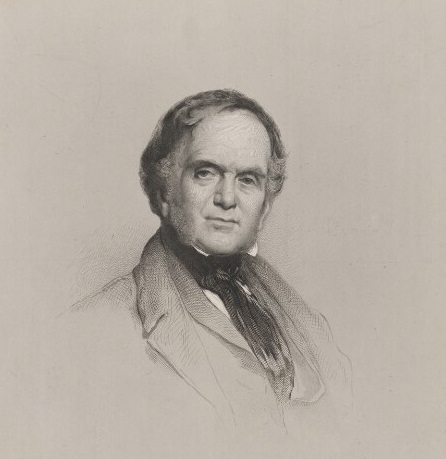
\includegraphics[scale=0.35]{figures/william_playfair.jpeg}
    \caption{William Playfair (1759-1823)}
    \label{fig:my_label4}
\end{figure}







A primeira metade do século XIX, conhecido com Início da Infografia Moderana (1800 à 1849), foi responsável por uma explosão no crescimento de gráficos estatísticos e de mapeamento temático, graças as inovações obtidas no século anterior. Todas as formas de gráficos estatísticos conhecidas hoje foram desenvolvidas nesta época, na cartografia, mapas simples foram transformados em atlas complexos baseados em grande variedade de dados.  
\vskip0.3cm

\inic Entre os anos de 1850 à 1900, conhecido como Era de Ouro da Estatística, onde as condições para um rápido crescimento das visualizações estavam estabelecidos. Escritórios de Análises se espalhavam pela Europa com o aumento da importância das informações numéricas para planejamento social, industria, comércio e transporte. A teoria estatística iniciada por GAUSS e LAPLACE deu os meios para fazer sentido a um grande número de dados.  
\vskip0.3cm 


\inic Compreendido entre 1900 à 1949, chamado de Período Negro do Gráficos de Estatística, aconteceram poucas inovações gráficas e o entusiasmo vivido no século passado foi suplantado pelo crescimento da quantificação e modelos formais. Durante esse período, no entanto, tudo que foi alcançado consegue se popularizar, seja no governo, no comércio e nas ciências. A visualização gráfica é consagrada para explicar novas descobertas e teorias.
\vskip0.3cm 


\inic De 1975 até hoje, o computador é considerado como nova fronteira. As inovações ocorridas nesta época foram muitas e em diversas áreas: o desenvolvimento de softwares e sistemas de computador,
altamente interativos e de fácil manipulação, foram a alavanca para tudo.\vskip0.3cm  

%Os novos paradigmas de manipulação de dados, a
%invenção de técnicas gráficas e os métodos de vizualização multidimensional deixaram suas marcas também.\vskip0.3cm  

\inic Com o surgimento da multimídia e da internet nos anos
1990 foram multiplicadas as formas de representar informação de modo dinâmico,
explorando animações, gráficos interativos e mapas com escala variável.







\section{Autores Importantes na Representação Gráfica}

\begin{itemize}
  \item O médico anestesista Britânico John Snow considerado o pai da epidemiologia moderna, em 1854, descobre a fonte transmissora de cólera e com um mapa registrou as coordenadas das ocorrências dos óbitos (SNOW, 1854a);
  \item Em 1858, Florence Nightingale, enfermeira britânica produziu o “coxcomb diagrams” que mostrou as baixas do exército britânico na Guerra da Criméia;
  \item Durante o ano de 1869, Charles Joseph Minard, engenheiro civil francês retratou a dizimação do exército de Napoleão durante sua condenada campanha contra a Rússia. Desmonstrando como níveis mais complexos de narratividades podem ser alcançados com uma única visualização estática (MINARD, 1869);
  \item No ano de 1914, Willard Brinton engenheiro americano publicou o primeiro livro de visualização para negócios;
  \item Em 1952, Mary Eleanor Spear publicou seu livro contendo boas práticas em construção de gráficos baseadas em décadas de serviço no governo Americano;
  \item Em 1967, Jacques Bertin, cartógrafo francês publicou o primeiro livro sobre teoria da visualização (Sémiologie graphique: Les diagrames, les
réseaux, les cartes), criava um sistema complexo de representação visual, com destaque para a cartografia. A semiologia gráfica era uma proposta arrojada para colocar problemas e apresentar dados de grande complexidade, longe de ser apenas ilustrativa (BERTIN, 1967); O livro era uma síntese de duas décadas de trabalho cotidiano na preparação de mapas para ilustrar livros de história e ciências sociais (GIL e BARLETA, 2015);
  \item  Em meados de 1970, John Tukey matemático americano foi pioneiro no uso de computadores para visualização e popularizou o conceito de visualização exploratória e confirmatória (TUKEY, 1997);
  \item Em 1983, Edward Rolf Tufte publicou em seu livro formas de combinar rigor estatístico com clareza e princípios de design gráfico, ou seja, a excelência em gráficos estatísticos consiste em idéias complexas comunicadas com clareza, precisão e eficiência (TUFTE, 1983);
  \item Em 1986, Jock Mackinlay publicou sua Tese de PhD que levou o trabalho de Jacques Bertin para era digital;
  \item Em 1999, Leland Wilkinson estabeleu uma grámatica concisa para
descrever os componentes de um gráfico.
\end{itemize}

\section{Porque usar Gráficos}

As estatísticas geralmente podem ser melhor compreendidas quando são apresentadas em um gráfico do que em uma tabela. Um gráfico é uma representação visual de dados estatísticos, em que os dados são representados por símbolos como barras ou linhas.
\vskip0.3cm  

É uma ferramenta visual muito eficaz, pois exibe os dados de forma rápida e fácil, facilita a comparação e pode revelar tendências e relacionamentos dentro dos dados.\vskip0.3cm  

Um gráfico geralmente assume a forma de uma figura uni ou bidimensional, como um gráfico de barras ou um gráfico de linhas. Embora existam gráficos tridimensionais disponíveis, eles geralmente são considerados complexos demais para serem facilmente compreendidos.\vskip0.3cm  

Os gráficos podem ser usados para ilustrar padrões em uma grande quantidade de dados ou para comunicar uma descoberta ou mensagem chave. Você deve considerar o uso de gráficos se quiser mostrar:

\begin{itemize}
    \item \textbf{Comparação}: Quantos? Qual item é maior ou menor?
    \item \textbf{Mudanças ao Longo do Tempo:} Como uma variável evolui?
    \item \textbf{Distribuição de frequência}: Como os itens são distribuídos? Quais são as diferenças?
    \item \textbf{Correlação}: Duas variáveis estão ligadas?
    \item \textbf{Participação relativa de um todo}: como um item se compara ao total
\end{itemize}


\section{Quando pode não ser apropriado usar gráficos}

Um gráfico nem sempre é a ferramenta mais adequada para apresentar informações estatísticas. \vskip0.3cm

Às vezes, um texto e/ou tabela de dados pode fornecer uma explicação melhor para o seu público e economizar tempo e esforço consideráveis.\vskip0.3cm

Você deve reconsiderar o uso de gráficos quando seus dados: 

\begin{itemize}
\item Estiverem muito dispersos; 
\item Têm poucos valores; 
\item Ter muitos valores; 
\item Mostram pouca ou nenhuma variação
\end{itemize}

%ROBINSON, Arthur. The look of maps: An examination of cartographic design. Wisconsin: University of Wisconsin Press, 1952


%SNOW, John. “The Principles on Which the Treatment of Cholera Should Be Based”. Medical Times and Gazette, n.8, 1854a,p.180-2.

%MINARD, Charles Joseph. Carte figurative des pertes successives en %hommes de l’Armée française dans la
%campagne de Russie 1812–1813. Paris: Regnier et Dourdet, 1869.

%TUFTE, Edward. The visual display of quantitative information. 2a edição. Cheshire, Conn.: Graphics
%Press, 2001; TUFTE, Edward. Envisioning information. Cheshire, Conn.: Graphics Press, 1995;

%TUKEY, John W. Exploratory data analysis. Reading, Mass.: Addison-Wesley Pub. Co., 1997

%1983: The Visual Display of Quantitative Information (pictures of numbers). ISBN 0-9613921-0-X

\newpage
\section{Conceitos Básicos de Representação Gráfica}

\inic Com palavras, números ou desenhos podem-se mostrar às pessoas interessadas o resultado da pesquisa, antes mesmo de aplicarem-se sobre os dados as operações matemáticas, que permitirão a interpretação final por parte da equipe encarregada do levantamento estatístico.\vskip0.3cm

A exposição por palavras é dita descritiva, a numérica é também conhecida como tabular e, finalmente, os desenhos constituem a exposição gráfica. Um relatório final reúne, quase sempre, as três modalidades de exposição, apresentando: gráficos, para ilustrar ou acentuar determinados itens: tabelas, para resumir a massa de dados observados no período de atividades; e palavras, para orientar a leitura, comentar as tabelas analisar os gráficos e concluir o relatório.\vskip0.3cm

Em muitas situações a apresentação gráfica é preferível a apresentação tabular. Os gráficos têm um impacto visual e uma facilidade de interpretação que o tornam muitas vezes mais úteis que as tabelas.\vskip0.3cm

A representação gráfica das séries estatísticas tem por finalidade representar os resultados obtidos, permitindo que se chegue a conclusões sobre a evolução do fenômeno ou sobre como se relacionam os valores da série. A escolha do gráfico mais apropriado ficará a critério do analista.\vskip0.3cm

As representações dos dados em sua forma gráfica constituem
importantes instrumentos de comunicação rápida, clara e efetiva,
poupando, sobretudo, tempo e esforço na visualização de dados
resumidos, permitindo fixar uma imagem duradoura, daí o largo uso
dessas representações em trabalhos científicos atualmente. (Ayres,
2003).\vskip0.3cm

A estatística gráfica são representações visuais dos dados
estatatísticos que devem corresponder, mas nunca substituir as
tabelas estatísticas.


\newpage
\section{Classificação Didática dos Gráficos}

\subsection{Quanto a Forma}

Há três tipos de gráficos, classificados quanto ao critério da forma:

\begin{enumerate}
  \item \textbf{Diagramas}: os diagramas são gráficos geométricos dispostos em duas dimensões. Os diagramas são os gráficos mais usados na representação de séries estatísticas e se  apresentam através de uma grande variedade de tipos.
\item \textbf{Cartogramas}: os cartogramas são ilustrações relativas a cartas geográficas, largamente difundidas em Geografia, História e Demografia.
\item \textbf{Estereogramas}: os estereogramas representam volumes e são apresentados em três dimensões. Muitas vezes são confeccionados em cartolinas ou madeira quando não desenhados em perspectiva.
\end{enumerate}

\subsection{Quanto ao Objetivo e Uso}

É possível distinguir, de certo modo arbitrariamente, dois objetivos que justificariam o emprego de gráficos. Os gráficos são usados para apresentar visualmente dados numéricos, proporcionando maior facilidade e rapidez de compreensão dos mesmos, ou, então, para apresentar conclusões ou resultados de uma análise. Há portanto, dois tipos de gráficos, conforme o objetivo ou uso a que se destinam: gráficos de informações e gráficos de análise.


\subsubsection{Gráfico de Informação}

\inic São gráficos destinados principalmente ao público em geral, objetivando proporcionar uma visualização rápida e clara da intensidade das modalidades e dos valores relativos ao fenômeno observado. São gráficos tipicamente expositivos, devendo, por conseguinte, ser o mais o completo possível, dispensando comentários explicativos adicionais. Nos gráficos de informação não se deve prescindir dos títulos. Já as legendas podem ser omitidas, desde que as informações desejadas  estejam presentes, possibilitando a completa interpretação do gráfico.

\subsubsection{Gráfico de Análise}

\inic Os gráficos de análise prestam-se melhor ao trabalho estatístico, fornecendo elementos úteis à fase de análise dos dados, sem deixar se ser também informativos. Quando se usam gráficos para apresentar os resultados de uma análise, esses freqüentemente vêm acompanhados de uma tabela. Inclui-se, muitas vezes, um texto dissertativo, chamando a atenção do leitor para os pontos principais revelados pelo gráfico ou pela tabela. Muitos relatórios administrativos, econômicos ou de qualquer outra natureza combinam as três formas de apresentação de dados. Isto porque, na prática, poucas pessoas têm habilidade com números, e as que têm dificuldades consultarão, via de regra, apenas o gráfico. Por outro lado, a maior parte das pessoas nunca examinará as tabelas estatísticas, preferindo analisar os gráficos e eventualmente procurar no texto a informação adicional necessária.\vskip0.3cm



















\section{Elementos  Básicos na Construção de Gráficos}

\inic Assim como tabelas, os gráficos devem ser referenciados no texto. Se eles ocorrem em um trabalho, é porque possuem alguma importância, fornecem alguma informação. Portanto, eles precisam ter alguma explicação ou comentário a respeito deles no corpo do trabalho.\vskip0.3cm 

\inic A representação gráfica deve conter determinados elementos que são essenciais para a sua compreensão, sendo esses elementos:

\section{Elementos Básicos}

\begin{itemize}
\item \textbf{Número}: utilizado para identificar o gráfico no
texto, sendo sempre precedido da palavra GRÁFICO com o seu número.
Por exemplo: GRÁFICO 1, GRÁFICO 2 etc, ou de acordo com a
numeração do capítulo, GRÁFICO 1.1, GRÁFICO 1.2, e assim por
diante. \item \textbf{Título}: deve conter designação do fenômeno
observado (O QUE?) e o local (ONDE?) e data de ocorrência do mesmo
(QUANDO?) e (COMO?), ficando abaixo do gráfico. O título deve
preferencialmente ser escrito após o número do gráfico, devendo
ser separado por espaço, hífen e espaço em letras maiúsculas
seguindo o padrão do texto. O título deve estar presente em qualquer tipo de representação gráfica a ser escrito com vista a orientar o leitor na sua interpretação. Simultaneamente, deve ser conciso, relevante e claro, ou seja, conter apenas informação essencial para uma interpretação correta do gráfico. 
\item \textbf{Fonte}: indicação do
órgão ou entidade responsável pelo fornecimento dos dados usados
na elaboração do gráfico. Utilizar letras maiúsculas para escrever
FONTE, devendo ser seguida de dois pontos, espaço e o nome da
fonte utilizada. Quando os dados foram obtidos pelo próprio autor,
por exemplo, em uma pesquisa e campo, a fonte pode ser escrita
como: FONTE: o autor. \item \textbf{Nota}: quando necessária, é
utilizada para a apresentação de informações de natureza geral,
esclarecendo o conteúdo ou metodologia utilizada. A nota vem em
seguida à fonte. A palavra NOTA deve ser escrita em letras
maiúsculas, devendo ser seguida de dois pontos, espaço e a
explicação da nota. \item \textbf{Nota Específica}: quando
necessária, é utilizada para esclarecer dados sobre um item ou uma
parte específica do gráfico; empregam-se chamada, indicadas no
gráfico, geralmente no titulo ou na legenda. A nota específica
deve ser chamada por algarismos arábicos entre parênteses.
\item \textbf{Legenda}: a legenda é constituída por símbolos e respectivas designinações. O procedimento dos sinbolos (cor ou outros) deve ser realizado de modo a que não haja lugar para qualquer confusão visual entre eles e, consequentemente, para que exista uma ligação clara entre os simbolos e a componente representada. As desiginações, por seu lado, devem ser claras e concisas, deixando para notas adjascentes eventuais esclarecimentos. Os símbolos devem aparecer na mesma ordem que as respectivas componentes: horizontalmente quando estão lado a lado e verticalmente quando estão umas sobre as outras (WALLGREN, 1996). Uma boa legenda deve fazer mais do que simplesmente etiquetar as componentes do gráfico. Deve dizer-nos o que é importante e qual é o objetivo do gráfico:   
informar o leitor e obrigar quem faz o gráfico a estruturar a informação (CLEVELANDO e MCGILL, 1984a).\vskip0.3cm

\item \textbf{Escalas}: Em um gráfico, as informações que possuem uma escala devem ser apresentadas com clareza. Os números da escala devem estar na posição horizontal e na região
externa dos eixos. A unidade de medida deve aparecer no final de cada linha do gráfico. Caso não seja possível apresentar a escala por completo, pode-se fazer um corte no eixo correspondente para informar que a escala não está completa.

\item \textbf{Linhas Auxiliares}: um dos elementos gráficos visualmente mais monótonos são as linhas auxiliares. devem, por isso ser suprimidas ou abafadas de tal forma que sua presença se torne implícita. Ainda que possam auxiliar a leitura dos dados, a maioria das linhas auxiliares escuras tem um grande peso visual, encobrindo muitas vezes, o mais importante do gráfico: a informação. Quando foram realmente necessárias deve-se optar por usar uma cor neutra e, no caso particular de um fundo branco, a cor cinzenta. Em certos caos em particular nas séries temporais, pode ser considerado importante incluir linhas auxiliares verticais como auxilio a leitura de valores por forma a complementar a leitura evolutiva da série com a leitura de valores em particular. Na maioria dos gráficos de séries temporais, os dados mais recentes estão situados à direita e longe das identificações do eixo dos valores, normalmente localizados à esquerda, fazendo com que o olho humano tenha que se movimentar alternadamente entre os dados e os valores ao longo das margens do gráfico. Esta imprecisão na leitura pode ser atenuada posicionando o eixo à direita junto dos dados mais recentes, duplicando o eixo, ou posicionando os valores junto das coordenadas respectivas (TUFTE, 1983).\vskip0.3cm

%\newpage

\inic Os gráficos com dois eixos distintos são normalmente utilizados quando se têm diferentes unidades de medida ou existem diferenças consideráveis de valores nas categorias de uma variável. Este tipo de gráficos deve ser evitado dado que é normalmente de difícil interpretação e, em muitos casos, bastante confuso (SCHMID, 1992). Por princípio, deve privilegiar-se a escala completa (com início em zero ou noutro valor de referência) em nome da honestidade na apresentação. Contudo, essa quebra é admissível nos casos em que a informação apresenta pequenas variações, desde que acompanhada por uma simbologia perceptível ao leitor. Para melhor compreender os dados na fase da análise exploratória não existe qualquer problema em manipular as escalas e extrapolar eventuais variações, mas na fase da divulgação, deve existir algum cuidado para não evidenciar graficamente alterações nos dados que na verdade não ocorreram. A quebra de escala é um exemplo de como se pode distorcer a mensagem transmitida. Quando o efeito nos dados é significativamente. 
\end{itemize}


\newpage
Quando se representa as informações de qualquer tipo de estudo em forma gráfica, precisam-se fazer algumas perguntas, tais como (VERGNAUD, 1987) e (WALLGREEN, 1996):

\begin{itemize}
\item Representar O Que? Para Quê?
\item Um gráfico realmente é a melhor opção?
\item Qual é o público alvo?
\item Qual é o objetivo do gráfico?
\item Que tipo de gráfico deve ser usado?
\item Como o gráfico deve ser apresentado?
\item Que tamanho o gráfico deve ter?
\item Deverá ser usado apenas um gráfico?
\item A qual meio técnico se deve recorrer?
\end{itemize}

Wallgreen(1996) acrescenta que a utilização gráfica apenas se pode
consumar após serem formuladas, e convenientemente respondidas, as
seguintes perguntas:

\begin{itemize}
\item O gráfico é fácil de ler? \item O gráfico pode ser mal
interpretado? \item O gráfico tem o tamanho e a forma certa? \item
O gráfico está localizado no local certo? \item O gráfico
beneficia por ser colorido? \item A compreenção do gráfico foi
testada com alguém?
\end{itemize}



\subsection{Requisitos Fundamentais de uma Representação Gráfica}

A representação gráfica de um fenômeno deve obdecer a certos
requisitos fundamentais para serem úteis.

\begin{enumerate}

\item \textbf{Compreensível}: permite visualizar as relações entre variáveis.
\item \textbf{Necessidade}: um gráfico deve ser útil para representar dados, deve haver uma necessidade para inserir elementos em um gráfico.
\item \textbf{Confiabilidade}: os dados devem estar corretamente representados, principalmente no que diz respeito a escala.
\item \textbf{Simplicidade}: deve ser destituída de detalhes de
importância secundária, assim como de traço desnecessários que
possam levar o observador a uma análise morosa ou com erros, ou
seja, a uma interpretação equivocada do fenômeno em estudo. \item
\textbf{Clareza}: deve possibilitar uma correta interpretação dos
valores representativos do fenômeno em estudo. \item
\textbf{Veracidade}: deve expressar a verdade sobre o fenômeno em
estudo.
\end{enumerate}


\newpage
\subsection{Diretrizes e Recomendações para a Construção de um Gráfico}

\begin{itemize}
\item O título do gráfico deve ser o mais claro e completo possível. Quando necessário, deve-se acrescentar subtítulos;
\item A orientação geral dos gráficos deve ser da esquerda para a direita;
\item As quantidades devem ser representadas por grandezas lineares;
\item Sempre que possível, a escala vertical há de ser escolhida de modo a aparecer a linha 0 (zero);
\item Só devem ser incluídas no desenho as coordenadas indispensáveis para guiar o olhar do leitor ao longo da leitura. Um tracejado muito cerrado dificulta o exame do gráfico;
\item A escala horizontal deve ser lida da esquerda para a direita, e a vertical de baixo para cima;
\item Os títulos e marcações do gráfico devem ser dispostos de maneira que sejam facilmente lidos, partindo da margem horizontal inferior ou da margem esquerda.
\item Um gráfico deve induzir o observador a pensar sobre o conteúdo e não no desenho do gráfico, na tecnologia ou outros atributos.
\item Induzir que os olhos do observador comparem diferentes partes dos dados.
\item Revelar diferentes detalhes dos dados, desde a perspectiva global até detalhes particulares (MAKINLAY, 1986).
\item Ter um objetivo bastante claro: descrição, exploração, tabulação e decoração.
\item Utilize uma linha de referência quando há algum valor importante que deva ser visto em todo o gráfico, por exemplo, uma linha média. Cuide para que isso não interfira na apresentação do gráfico.
\item Elimine da visualização gráficos e textos desnecessários. Uma boa medida de
quantos elementos são desnecessários em uma figura é a quantidade de tinta ou de
pixels gastos com itens que não são dados de interesse.
\item Explore a utilização de símbolos e de atributos visuais que facilitem a percepção
dos dados e dos padrões existentes nos mesmos.
\end{itemize}

\newpage
\subsection{Sugestões de Leitura e Interpretação de um Gráfico}

\begin{itemize}
\item Declarar qual o fenômeno ou fenômenos representados, a
região considerada, o período de tempo, a fonte dos dados, etc;
\item Examinar o tipo de gráfico escolhido, verificar se é o mais
adequado, criticar a sua execução, no conjunto e nos detalhes;
\item Analisar cada fenômeno separadamente, fazendo notar os
pontos mais em evidência, o máximo e o mínimo, assim como as
mudanças mais bruscas; \item Investigar se há uma "tendência
geral" crescente ou decrescente ou, então, se o fato exposto é
estacionário; \item Procurar descobrir a existência de possíveis
ciclos periódicos, qual o período aproximado, etc. \item Quando um
gráfico for inserido em um texto, recomenda-se que este seja
destacado tanto do texto que o precede, como do texto imediamente
subsequente, por meio de três espaços simples. \item Com relação a
variação das cores num mesmo gráfico é recomendada para o caso de
gráficos comparativos, dos quais, se dá preferência a pouca
variação de cores.
\end{itemize}

O verdadeiro desafio é saber apresentar os dados de forma interessante e atrativa. Contudo, construir gráficos e mapas estimulantes e cientificamente corretos não é tarefa tão fácil como pode parecer. Não basta ter os dados e saber usar os programas informáticos. É preciso saber transformá-los numa história bem contada e transmitir idéias e fenômenos que dificilmente seriam visíveis de outra forma.

\newpage
\subsection{Principais Erros Encontrados em um Gráfico}
\inic Os problemas mais comuns que podem comprometer a efetividade de uma visualização gráfica são:


\begin{itemize}
\item Em geral o excesso de decoração é um problema.
\item Ausência ou erro na escala de eixos.
\item Ausência de um título, marcas e indicadores.
\item Não Colocar dados suficientes na visualização de forma a contextualizar as informações mais relevantes apresentadas.
\item Excesso de informação.
\item  Utilizar gráficos sobrepostos em escalas diferentes ou com sistemas de coordenadas distintos, o que impede uma comparação justa entre os dados.
\item Não fazer um mapeamento dos dados para marcas e atributos visuais de forma adequada.
\end{itemize}



\newpage
\section{Principais Tipos de Gráficos}

\subsection{Ramo-e-Folhas}

Os gráficos chamados de ramo-e-folhas, talo-e-folhas ou \textit{Stem and leaf} foram criados em 1977 pelo estatístico americano Jhon Tukey. O mesmo fornece um meio prático de registrar as observações e podem ser usados como uma amostra direta dos dados ou um passo preliminar ma construção de uma tabela de frequência.\vst






Para a construção de um gráfico ramo-e-folhas, não há regras fixas para construi-los, mas a idéia básica é dividir cada observação em duas partes: desenhe uma linha vertical e coloque os primeiros digitos de cada classe (chamados de ramos) no lado esquerdo da linha vertical. Os números no lado direito da linha vertical representam o segundo dígito de cada observação, sendo estes as folhas.


% figura 1

%\begin{figure}
%   \centering
%    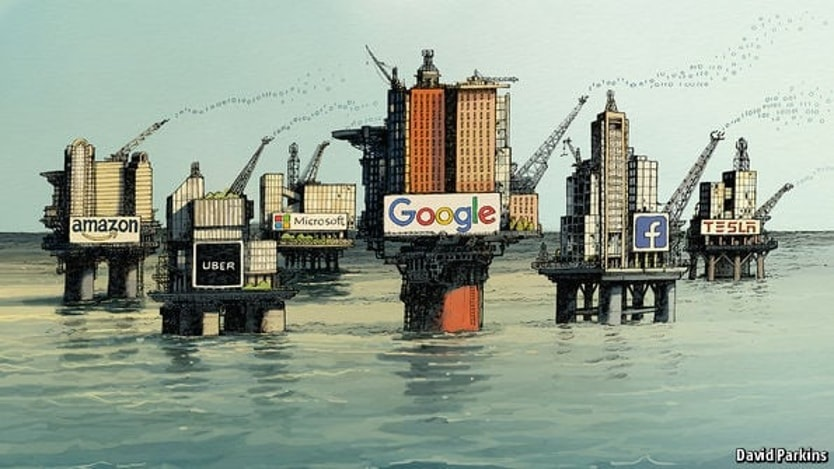
\includegraphics[scale=0.5]{figures/dados1.jpeg}
%    \caption{Caption}
%    \label{fig:my_label}
%\end{figure}


\newpage
\subsection{Histogramas}

\inic O histograma é um gráfico de barras no qual a escala horizontal representa classes de valores de dados e a escala vertical representa frequências. As alturas dos barras correspondem aos valores das frequências, e as barras são desenhadas adjascente uma às outras (sem separação).
 \vskip0.3cm
 
\inic O histograma é formado por um conjunto de retangulos justapostos
que tem as bases sobre um eixo horizontal, com centro no ponto
médio. As bases coincidem com as amplitudes de classe, e as
alturas devem ser proporcionais as frequências das
classes.
\vskip0.3cm 
 

\inic Os histogramas em geral apresentam a medição de interesse no eixo
x e o número ou percentagem de observações no eixo y, embora
alguns programas de computador façam o oposto. 
\vskip0.3cm

Se todos os intervalos tiverem a mesma amplitude, as alturas serão
proporcionais as frequências das classes, tornando-se então as
alturas numericamente iguais a essas frequências.\vskip0.3cm

ou seja,\vskip0.3cm

LARGURA DO RETÂNGULO = h(amplitude de classe)

ALTURA DO RETÂNGULO = f(frequência de classe)


% Histograma 1

%\begin{figure}
%    \centering
%    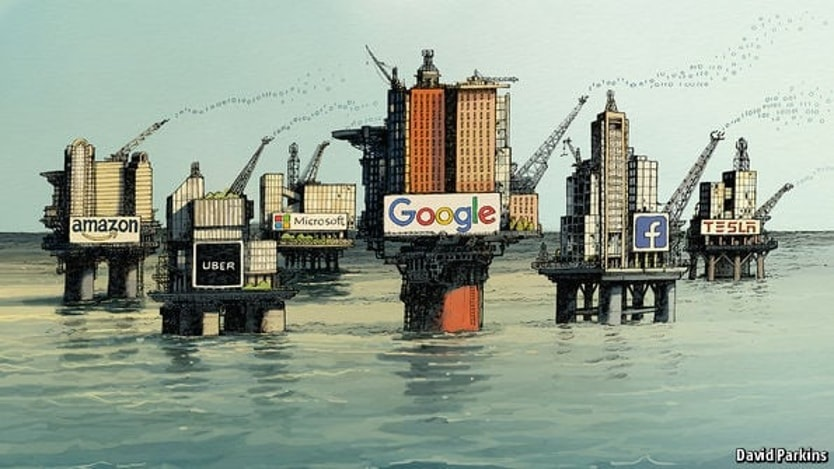
\includegraphics[scale=0.5]{figures/dados1.jpeg}
%    \caption{Caption}
%    \label{fig:my_label}
%\end{figure}





\newpage
\subsection{Polígono de Frequência Simples e Acumulado}

\inic È um gráfico de linhas, sendo as frequência marcadas sobre as
perpendiculares levantadas pelos pontos médios das classes.\vskip0.3cm

È a representação gráfica das frequências acumuladas. Usa-se
quando deseja saber qual parcela da população encontra-se até um
determinado valor, ou qual parcela encontra-se após um determinado
valor.\vskip0.3cm

O polígono de frequência é traçado marcando-se as frequências
acumuladas sobre os pontos correspondente aos limites superiores
dos intervalos de classe, também, conhecido como \textbf{Ogiva de
Galton}. A partir da Ogiva de Galton, pode-se fazer uma
interpolação linear, estimar valores de frequências acumuladas, de
uma distribuição em classes de frequências.\vskip0.3cm

A ogiva de galton, ou também chamada de \textbf{Gráfico de
Frequências Acumuladas}, concentra no limite superior de cada
classe a quantidade de elementos inferiores ou iguais a esse
limite superior. Dessa, forma, pode-se estimar a frequência
acumulada para um determinado valor que pertença a qualquer
intervalo que tiver sido usado para construir a ogiva. Para
determinadar esse valor, faz-se uma interpolação linear da ogiva.

\newpage
\subsection{Gráfico de Barras (Simples ou Múltiplas)}

\inic O gráfico de barras é composto por duas linhas ou eixos, um
vertical e outro horizontal. No eixo vertical são construídas as
barras que representam a variação de um fenômeno ou de um processo
de acordo com sua intensidade. Essa intensidade é indicada pela
altura da barra. No eixo horizontal especifica-se as categorias da
variavel. As barras devem sempre possuir a mesma largura e a
distância entre elas deve ser constante.\vskip0.3cm

Os Gráficos de Barra são uma das formas mais populares de representar a informação, principalmente pela facilidade de execução e leitura. Sendo utilizado para apresentar um conjunto de dados e também para comparar vários conjuntos de dados. O formato em barras devem ser utilizados para representar variáveis discretas ou qualitativas, em termos absolutos ou relativos, para comparar categorias de variáveis quantitativas ou representar a evolução de uma característica ao longo do tempo.\vskip0.3cm

A representação de valores negativos é desaconselhada em gráficos de barras, dado que, convencionalmente, aos valores negativos está associada uma barra numa posição descendente. De fato, a associação visual entre esquerda e direita e valores negativos e positivos, respectivamente, pode não ser directa para um leitor menos experiente. Por essa razão, devem ser utilizados gráficos de colunas quando existem valores negativos.\vskip0.3cm

Nos gráficos de barras não é admissível a quebra de escala por deixar de ser possível efectuar comparações verticais entre categorias. Uma quebra de escala é enganadora, porque mostra visualmente a existência de grandes variações nos dados que de fato, não existem.\vskip0.3cm 

Na representação da informação, por vezes, é importante organizar as categorias por ordem crescente ou decrescente para melhor compreender certos fenómenos implícitos. É igualmente comum ordenar alfabeticamente (ou geograficamente) as designações das categorias, nomeadamente nos casos em que se representam países ou outro tipo de unidades administrativas, mas tal nem sempre é a melhor opção. Se o mesmo conjunto de categorias é apresentado em mais do que um gráfico, então a posição relativa de cada categoria deve manter-se, ou seja, as categorias devem aparecer na mesma ordem em todos os gráficos. Da mesma forma, o tamanho e a escala dos gráficos deve ser o mesmo, se o objectivo for a comparação entre eles. \vskip0.3cm  

Quando as categorias não são todas discriminadas, existindo, por exemplo, uma que reúne as restantes categorias sob a designação de ‘Outros’, é aconselhável não a incluir na ordenação e reservar-lhe o último lugar (WALLGREN, 1996; SCHMID, 1992). Caso se utilizem cores para diferenciar as categorias, a categoria ‘Outros’, por ser a menos importante, deve ter uma cor que não se destaque (ex: cinzento). \vskip0.3cm

\inic O primeiro passo na construção do gráfico é ter os dados armazenados em objetos apropriados. No caso do gráfico de barras é necessário que os dados estejam armazenados em um vetor ou matriz.




%\inic Pode-se criar também, o gráfico de barras de duas ou mais
%variáveis, um ao lado do outro, na mesma janela gráfica.
%\subsection{Gráfico de Colunas (Simples ou Multiplas)}


\newpage
\subsection{Gráfico de Linhas, Curvas ou Segmentos}

Este tipo de gráfico representa a série histórica, exclusivamente,
indicado para mostrar tendências e evolução de uma variável
contínua por outra variável contínua. Requer, entretanto, que tal
série apresente um número significativo de informações (5 ou
mais), ou melhor, para 5 ou número menor de ocorrências, outro
gráfico deve ser construído, o gráfico de colunas.\vskip0.3cm

O primeiro gráfico data do séc. X ou XI, mas só no fim do séc. XVIII surgiu na literatura. William Playfair foi responsável pela publicação do primeiro gráfico de linhas baseado em dados económicos. A reintrodução do sistema de coordenadas cartesianas em 1637 por René Decartes, responsável pela relação estabelecida entre uma linha e uma equação, enquadrou e deu corpo a este formato de representação de dados.\vskip0.3cm

A leitura dos dados em gráficos de séries temporais obedece a duas lógicas preferenciais: avaliação da tendência, crescente ou decrescente, da série de dados, e responder a perguntas do tipo: Em que período se localizou o maior aumento ou a maior diminuição? Quais foram os pontos de inflexão ou de inversão pontual da tendência? A escala logarítmica possibilita a comparação de séries cujos valores apresentam dimensões muito diferentes (ainda que os valores da escala deixem de poder ser lidos de forma direta). Em certas circunstâncias, deve ser equacionada a substituição destes formatos pelos gráficos de barras e gráficos de área.

\newpage
\subsection{Gráfico Circular, Setorial ou Pizza}

O gráfico circular, setorial ou também chamado de Pizza, é
utilizado para comparar os valores de cada parcela de um conjunto
de dados com o total. É feito tomando por base a figura de um
círculo dividido em setores de tamanhos proporcionais aos valores
que representam. Os valores são expressos em números ou em percentuais. \vskip0.3cm

Algumas recomendações devem ser feitas para a elaboração dos
gráficos setoriais. Os valores devem ser apresentados em ordem
decrescente a partir da parte superior do gráfico e no sentido
horário.\vskip0.3cm

A sua utilização é desaconselhada quando se pretende comparar mais
de um período temporal, para variáveis que contenham até cinco
categorias ou quando as categorias têm aproximadamente o mesmo
peso, sob pena de perder umas das principais funçoes: a da
comparação, sendo neste caso, preferível substituir o gráfico de
setores por um gráfico de barras.


\newpage
\subsection{Gráfico Polar}

È a representação de uma série histórica ou temporal por meio de
círculos concêntricos divididos em setores de iguais dimensões e
em quantidades, de acordo com a variabilidade do fato estudado. A
representação dos dados resultará na composição ou de um polígono
ou do traçado de linhas radiais proporcionais aos valores que
representam, as quais servirão de recursos visuais para a
interpretação das informações. Muito utilizados para a
representação de dados sobre abordagens de operações da Lei Seca
pelos agentes de fiscalização de forma mensal.



\newpage
\subsection{Gráfico Triangular ou Radar}

O gráfico triangular é utilizado para representar fenômenos cuja
apresentação é feita em três variáveis. A sua análise exige mais
atenção em virtude da maior complexidade da sua apresentação. Tem
sido muito utilizado para representar fenômenos como estrutura
fundiária, composição etária da população, população
economicamente ativa, composição do solo e outros.


\newpage
\subsection{Gráfico em Pirâmide Etária}

A pirâmide etária é também um histograma e é muito utilizada em  análises demográficas por permitir visualizar numa única imagem a distribuição da população por idades e silutaneamente compará-las entre os gêneros. A representação em valores absolutos fornece a dimensão dos dados mas impede qualquer tipo de comparação no espaço ou no tempo, que apenas é possível se os dados foram apresentados em termos relativos (NAZARETH, 1996). 
\vskip0.3cm

A pirâmide etária é uma forma de representar a estrutura da
população por idade e gênero. O eixo horizontal representa o
número absoluto ou relativo da população e o eixo vertical
representa os grupos etários e são normalmente apresentados em grupos etários em cinco anos, mas também podem ser representados ano a ano. O lado direito do eixo horizontal é destinado à representação do contingente ou proporção de mulheres e o esquerdo, dos homens.


\newpage
\subsection{Gráfico em Cartograma}

O cartograma é a representação sobre uma carta geográfica (mapa).
Também chamado de Estegráfico é empregado quando o objetivo é o de
figurar os dados estatísticos diretamente relacionados com áreas
geográficas ou políticas


\newpage
\subsection{Gráfico Ilustrativo, Diagrama Símbólico, Pictórico ou Pictograma}

O pictograma constitui um dos processos gráficos que melhor fala
ao público, pela sua forma ao mesmo tempo atraente e sugestiva. O
pictograma é um gráfico representado através de figuras que
simbolizam fatos estatísticos, ao mesmo tempo que indicam
proporcionalidade. São gráficos que carecem de precisão, mas, como
são muitos atrativos, são largamente usados em revistas voltadas
ao público em geral e publicidades na segurança pública. Não é
utilizado em trabalhos científicos.\vskip0.3cm

Os diagramas simbólicos são frequentemente usados para apresentar os dados estatísticos de modo a despertar a atenção do público em geral, e apresentando grande dose de originalidade e de habilidade na arte de apresentação dos dados.\vskip0.3cm

Os pictogramas mais usuais são os baseados no critério do tamanho: em que a variação em área do tamanho das formas utilizadas é proporcional à variação da variável representada.\vskip0.3cm



\textbf{Regras Fundamentais para a Construção de um Pictograma}

\begin{enumerate}
    \item Os símbolos devem explicar-se por si próprios.
    \item As quantidades maiores são indicadas por meio de um
    número maior de símbolos, mas não por um símbolo maior.
    \item Os símbolos comparam quantidades aproximadas, não
    detalhes minuciosos.
    \item Os gráficos pictóricos só devem ser usados para
    comparações, nunca para afirmações detalhadas ou isoladas.
\end{enumerate}


\newpage 
\subsection{Diagrama de Caixa, Bigodes, Whisker ou Box Plot}

\inic Em 1977, o estatístico John Wilder Tukey propôs um dispositivo visual útil
para a comunicação de características de uma série de dados que se
tornou bastante famoso. Conhecido enormemente no meio acadêmico
como Box-Plot, na qual é um tipo de gráfico que objetiva
apresentar diversas informações sobre o comportamento dos dados e
ainda manter uma forma compacta. Na análise das informações, pode
ser importante a construção de um diagrama em caixa, contendo as
seguintes informações: valores mínimos e máximos, a mediana, o
primeiro e o terceiro quartil, na qual representa 25\% e 75\% da
distribuição de freqüência.\vskip0.3cm


\vspace{-2cm}
\begin{figure}
    \centering
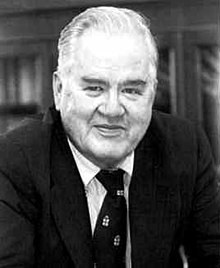
\includegraphics[scale=0.65]{figures/John_Tukey.jpeg}
    \caption{John Wilder Tukey (1915-2000)}
    \label{fig:my_label25}
\end{figure}




%\begin{figure}[!htb]
%\centering{
%  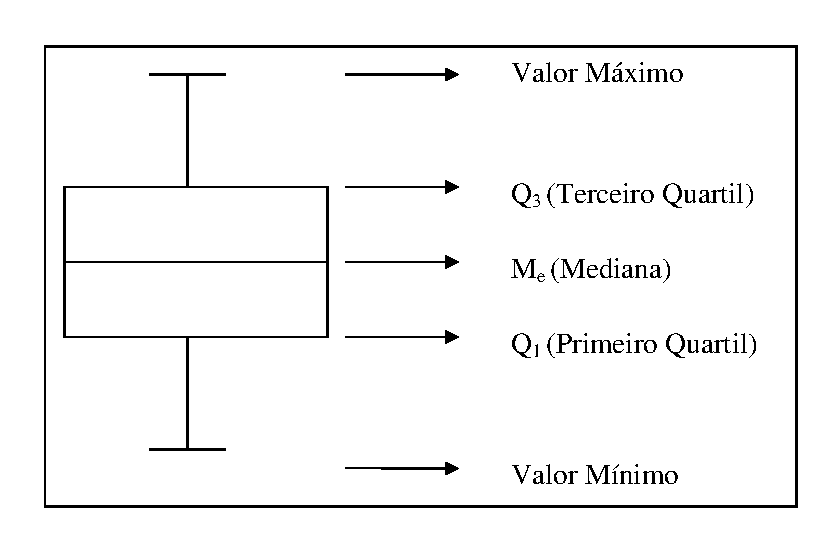
\includegraphics[scale=0.85]{figures/Boxcaixa.eps}\\
%  \vspace{-0.2cm}
%  \caption{Esquema Geral sobre o diagrama de caixas ou Box Plot.}\label{esquematabela}
%  }
%\end{figure}



\inic As linhas verticais que saem do diagrama foram chamadas whiskers
por Tukey, essas linhas servem de elo entre os valores mais
centrais e os extremos da série de dados, geralmente representam
os valores mínimos e máximos. A mediana da série é representada
por uma linha horizontal central no diagrama, e o quartil inferior
(Q1) e superior (Q3), pelas linhas inferior e superior que
delimitam a caixa. A mediana representa uma estimativa de tendência central, e a altura da do diagrama, uma estimativa da variabilidade geral dos
dados. Na qual a posição da mediana, seja ela central ou mais
próxima a um dos quartis, indica a presença ou não de assimetria
nos dados.\vskip0.3cm

\inic Ao explorar um conjunto de dados de forma gráfica, deve-se considerar os valores discrepantes ou Outliers, pois eles podem revelar importantes informações e podem afetar grandemente os valores da média e do desvio-padrão, bem como disfarçar seriamente um histograma, ou seja,, um outlier pode ter efeito um dramático sobre a escala do gráfico, de modo que a verdadeira natureza da distribuição pode ser totalmente  obscurecida.















\subsection{Resumo Geral Sobre os Principais Gráficos}

\inic Atualmente existem diversos tipos de gráficos, onde a escolha depende do tipo de dado coletado e da informação que se pretende transmitir. Cada um possui um conjunto de vantagens e desvantagens.      

\begin{quadro}[h!tp]
    \centering
    \caption{Resumo geral sobre os principais gráficos mostrando suas descrição, vantagens e desvantagens}
    \begin{tabular}{|c|c|c|c|}
   \hline\hline
    Gráficos       & Descrição &  Vantagens & Desvantagens \\   
\hline\hline
  Barras           &           &           &             \\
  Barras Agrupadas &           &           &              \\
  Linhas           &           &           &              \\  
  Setores          &           &           &              \\
  Histograma       &           &           &              \\
  Polígono         &           &           &              \\
  Box Plot         &           &           &              \\
\hline\hline
\end{tabular}
\end{quadro}










\setcounter{chapter}{5} \chapter{Principais Medidas Estatísticas}

\section{Introdução}

Algumas medidas de suma importância para a estatística são os somatórios e produtórios. Suas aplicabilidades vão desde a estatística descritiva, análise de variância, ao desenvolvimento de funções. Estes temas serão tratados a seguir.


\subsection{Somatório Simples}

\inic Muitos dos processos estatísticos exigem o cálculo da soma. Para simplificar a representação da operação de adição nas expressões algébricas, utiliza-se a notação representada pela letra grega sigma maiúsculo ($\Sigma$), na qual o somatório foi proposto para simplificar a representação da soma.\vskip0.3cm


Assim, $\sum_{i=1}^{n}x_{i}$  lê-se  somatório de x índice i, com i variando de 1 até n, em que n é a ordem da ultima parcela da soma ou o limite superior (LS) do somatório, i=1 é a ordem da primeira parcela da soma ou o limite inferior (LI), e i é o índice que está indexando os valores da variável  X (ou letras como Y, Z, W podem ser utilizadas).\vskip0.3cm

As letras do meio do alfabeto são geralmente usadas como índices, letras do final do alfabeto são comumente utilizadas como variáveis; e letras do inicio do alfabeto são freqüentemente empregadas para representar eventos em cálculo de probabilidades. Na verdade, o somatório nada mais é do que uma notação simplificada de várias somas.\vskip0.3cm

As principais representações dos somatórios são:


$$\sum_{i=1}^{n}x_{i} = (x_{1}+x_{2}+\ldots+x_{n}) \ \ Soma \ \ Simples $$

$$\sum_{i=1}^{n}x_{i}^{2} = (x_{1}^{2}+x_{2}^{2}+\ldots+x_{n}^{2}) \ \ Soma \ de \ Quadrados$$


$$ \left(\sum_{i=1}^{n}x_{i}\right)^{2}=(x_{i}+x_{2}+\ldots+x_{n})^{2} \ \ Quadrado \ da \ Soma$$

$$ \sum_{i=1}^{n}x_{i}y_{j}= \left( (x_{1}y_{1})+(x_{2}y_{2})+\ldots+(x_{n}y_{n}) \right) \ \ Soma \ de \ Produtos$$

$$ \sum_{i=1}^{n}x_{i} \sum_{j=1}^{m}y_{j}= (x_{1}+x_{2}+\ldots+x_{n})(y_{1}+y_{2}+\ldots+y_{n}) \ \ Produto \ da \ Soma$$


\subsection{Proriedades do Somatório}

\begin{enumerate}
  \item [{a})] O número de termos (NT) de um somatório refere-se à diferença entre os limites superior (ls) e inferior (li) acrescido da unidade, ou adicionalmente decrescido de r, quando o somatório estiver sujeito a r restrições.
\begin{equation}\label{}
    NT=(LS-LI)+1-r
\end{equation}
  \item [{b})] O somatório de uma constante k refere-se ao produto de NT por k.
$$\sum_{i=1}^{n}k=[(n-1)+1]k = nk $$
ou
$$ \sum_{i=1}^{n}k = (k+k+\ldots+k) = nk $$
  \item [{c})] O Somatório do produto de uma constante por uma variável que depende do somatório é igual ao produto da constate pelo somatório da variável, ou seja,
$$ \sum_{i=1}^{n}(kx_{i}) = (kx_{1}+kx_{2}+\ldots+kx_{n}) = k \left( \sum_{i=1}^{n} \right)$$
      \item [{d})] Propriedade Distributiva com relação à adição, isto é
$$ \sum_{i=1}^{n}(x_{i}+y_{j}) = \left( \sum_{i=1}^{n}x_{i} \right) + \left( \sum_{i=1}^{n}y_{i} \right) $$
  \item [{e})] Propriedade Distributiva com relação à subtração, isto é
$$ \sum_{i=1}^{n}(x_{i}-y_{j}) = \left( \sum_{i=1}^{n}x_{i}\right) - \left( \sum_{i=1}^{n}y_{i}  \right) $$
  \item [{f})] O Quadrado da soma é diferente da soma dos quadrados, ou seja,
  $$\left(\sum_{i=1}^{n}x_{i}\right)^{2} \neq  \left( \sum_{i=1}^{n}x_{i}^{2} \right)$$
  \item [{g})] O Produto de duas somas é diferente da soma dos produtos, isto é
  $$ \left[ \left(\sum_{i=1}^{n}x_{i} \right) \times \left(\sum_{i=1}^{n}y_{i} \right) \right] \neq  \left( \sum_{i=1}^{n} (x_{i} \times y_{i})\right) $$
  \item [{h})] O somatório de um quociente é diferente do quociente de duas somas.
$$  \left( \sum_{i=1}^{n} \frac{x_{i}}{y_{i}} \right) \neq \left( \frac{\sum_{i=1}^{n}x_{i}}{\sum_{i=1}^{n}y_{i}} \right) $$
  \item [{i})] O somatório duplo de um produto é igual ao produto dos somatórios tomados separadamente.
  $$   \left( \sum_{i=1}^{n} \sum_{j=1}^{m}x_{i}y_{j} \right)  =  \left( \sum_{i=1}^{n}x_{i} \times \sum_{j=1}^{m}y_{i} \right) $$
\end{enumerate}




\subsection{Somatório Duplo}

Acontece com muita freqüência, na apresentação de dados estatísticos, o emprego de tabelas de dupla entrada, nas quais os valores são expressos em função de duas variáveis: uma variável linha e uma coluna. Desta maneira pode-se representar: estado civil (solteiro, casado, outros) versus o gênero (masculinoe feminino), as faixas etárias versus suas rendas, componentes versus modelos, etc. Assim, a indicação da soma dos elementos das tabelas de dupla entrada pode ser feita mediante o emprego do somatório duplo.\vskip0.3cm








\newpage

%\textbf{Exercícios de Somatório:}


%\begin{enumerate}
%  \item [{1)}] Sabe-se que: \\
%  $X_{1}=3$ $X_{2}=4$ $X_{3}=8$ $X_{4}=7$ $X_{5}=6$\\
%  $Y_{1}=3$ $Y_{2}=8$ $Y_{3}=2$ $Y_{4}=5$ $Y_{5}=6$\\
%  Calcule:
%  \begin{enumerate}
%    \item [{a)}] $\sum_{i=1}^{5}X_{i}$
%    \item [{b)}] $\sum_{i=1}^{5} 4 X_{i}$
%    \item [{c)}] $\sum_{i=3}^{5} (X_{i}+6)$
%    \item [{d)}] $\sum_{i=2}^{4} (2X_{i}-3)$
%    \item [{e)}] $\sum_{i=1}^{5}X_{i}Y_{i}$
%    \item [{f)}] $\sum_{i=1}^{5}(X_{i}+Y_{i})$
%  \end{enumerate}
%  \item [{2)}] Se o $\sum_{i=1}^{6}X_{i}=-4$ e %$\sum_{i=1}^{6}X_{i}^{2}=10$, calcular as seguintes expressões
%  \begin{enumerate}
%    \item [{a)}] $\sum_{i=1}^{6}(2X_{i}+3)$
%   \item [{b)}] $\sum_{i=1}^{6}(X_{i}-1)$
%   \item [{c)}] $\sum_{i=1}^{6}(X_{i}-5)^{2}$
%   \end{enumerate}
%  \item [{3)}] Dados $\sum_{i=1}^{4}X_{i}=7$, %$\sum_{i=1}^{4}Y_{i}=-3$ e $\sum_{i=1}^{4}X_{i}Y_{i}=5$, %determinar:
%  \begin{enumerate}
%    \item [{a)}] $\sum_{i=1}^{4}(2X_{i}+5X_{i})$
%    \item [{b)}] $\sum_{i=1}^{4}(X_{i}-3)(2Y_{i}+1)$
%   \end{enumerate}
%  \item [{4)}] Desenvolver os termos de cada uma das seguintes %somas indicadas:
%  \begin{enumerate}
%   \item [{a)}] $\sum_{i=1}^{n}a$
%    \item [{b)}] $ \sum_{i-1}^{6}X_{i}^{2}$
%    \item [{c)}] $\sum_{i=1}^{4}(Y_{1}-3)^{2} $
%    \item [{d)}] $\sum_{i=1}^{5}F_{i}X_{i} $
%    \item [{e)}] $\sum_{i=1}^{4}(X_{i}+Y_{i}) $
%    \item [{f)}] $\sum_{i=1}^{4}(\frac{X_{1}}{Y_{i}}-1)^{2} $
%    \item [{g)}] $\sum_{i=1}^{3}(X_{i}-a)$
%    \item [{h)}] $\sum_{i=1}^{5}f_{1}(Y_{i}-a)^{2}$
%  \end{enumerate}
%  \item [{5)}] Se $Z_{1}=X_{1}+Y_{1}$ e $Z_{2}=X_{2}+Y_{2} %\ldots Z_{n}=X_{n}+Y_{n}$, Provar que $\bar{Z}=\bar{X}+\bar{Y}$
%  \item [{6)}] Demonstrar que:
%  \begin{enumerate}
%    \item [{a)}] $\sum_{i=1}^{n}(X_{i}-\bar{X})=0$
%    \item [{b)}] $\sum_{i=1}^{n}(X_{i}-a)= Minimo$
%    \item [{c)}] $\sum_{i=1}^{n}X_{i}(X_{i}-%\bar{X})=\sum_{i=1}^{n}(X_{i}-\bar{X})^{2}$
%    \item [{d)}] $\sum_{i=1}^{n}[X_{1}(X_{i}+\bar{X})-%\bar{X}^{2}]=\sum_{i=1}^{n}X_{i=1}^{2}$
%    \item [{e)}] $\sum_{i=1}^{n}\sum_{j=1}^{n}(X_{i}-\bar{X})
%(Y_{j}-\bar{Y})=0$
%    \item [{f)}] $\sum_{i=1}^{n}[X_{i}(X_{i}+\bar{X})+(X_{i}-%\bar{X})^{2}]=2\sum_{j=1}^{n}X_{j}^{2}$
%    \item [{g)}] $\sum_{i=1}^{N}
%(X_{i}-1)^{2}=\sum_{i=1}^{N}X_{i}^{2}-2\sum_{i=1}^{N}+N$
%    \item [{h)}] $\sum f_{i}(x_{i}-\bar{x})^{2}= \sum %f_{i}x_{i}^{2}- \frac{(\sum f_{i}x_{i})^{2}}{\sum f_{i}}$
%  \end{enumerate}
%\end{enumerate}






\subsection{Produtório}

O símbolo produtório foi proposto para simplificar e facilitar a representação dos produtos nas expressões algébricas. Representado pela letra grega $pi$ maiúscula ($\Pi$).


\begin{equation}\label{}
    \prod_{i=1}^{n}x_{i} = (x_{1} \times x_{2} \times  \ldots \times x_{n})
\end{equation}


Lê-se: produtório de X índice i, com i variando de 1 a n.

\vskip0.3cm

ou seja,

\begin{equation}\label{}
    \underbrace{x_{1} \times x_{2} \times  \ldots \times x_{n}}_{n fatores}= \prod_{i=1}^{n}x_{i}= x^{n}
\end{equation}









\subsection{Proporções e Percentagens}


Uma proporção é o número, $a$, de observações com determinada caracteristica (como por exemplo aqueles que sofreram um acidente de trânsito) dividido pelo número total de observações, $a+b$, num determinado grupo (como aqueles que estão na condição de Motociclistas). Isto é,


$$ 
\mbox{Proporção} = \left( \frac{a}{a+b} \right)
$$

Uma proporção sempre é definida como uma parte dividida pelo total e é útil para dados ordinais e números assim como para dados nominais, especialmente quando as observações forem colocadas numa tabela de frequência. Uma \textbf{Percentagem} é a proporção multiplicada por $100\%$.\vskip0.3cm


$$ \mbox{Proporção} = \left( \frac{a}{a+b} \right) \times 100\% $$

\newpage
\subsection{Razões}

Uma razão é o número $a$ de observações num determinado grupo com cada característica
dividida pelo número b de observações sem essa característica:


$$ 
\mbox{Razão} = \left( \frac{a}{b} \right)
$$

Uma razão sempre é definida como uma parte dividida por uma outra parte.\vskip0.3cm

\subsection{Taxas}

As Taxas são semelhantes as proporções exceto pelo fato de que é usado um multiplicador ($1.000 , 10.000 , ou 100.000$) e são calculados durante um período específico. O multiplicador é chamado de base e a fórmula é


$$ 
\mbox{Taxa} = \left( \frac{a}{a+b} \right) \times base
$$



\subsection{Coeficientes}

É a relação entre o número de eventos reais (os acontecimentos) e os esperados (que poderiam acontecer). È a medida de probabilidade. O numerador exprime o número de eventos ocorridos e o denominador exprime a população efetivamente exposta ao evento.\vskip0.3cm

Apresenta-se a seguir alguns exemplos de coeficientes.

\subsubsection{Coeficiente de Mortalidade Geral - CMG}

$$
C_{M_{G}} = \left(  \frac{numero \ de \ total \ de \ obitos \ em \ certa \ area \ durante \ o \ ano}{populacao \ da \ mesma \ area \ ajustada \ para \ o \ meio \ do \ ano} \right) \times 1.000
$$











\newpage
\section{Medidas de Tendência Central, Localização ou Posição}

Torna-se necessário, após a tabulação dos resultados e da representação gráfica, encontrar valores que possam representar a distribuição como um todo. São as chamadas medidas de tendência central, de posição ou localização.\vskip0.3cm

As medidas da tendência central são indicadores que permitem onde se tenha uma primeira idéia, um resumo, de como se distribuem os dados num experimento, informando o valor (ou faixa de valores) da variável aleatória que ocorre mais tipicamente, ou seja, compõem-se de um número que representa um conjunto particular de informações, geralmente, se localizam em torno do centro da distribuição, onde a maior parte das observações tende a concentrar-se.





\subsection{Média Aritmética Simples ($\bar{X}$)}

A média procura substituir um conjunto de valores por um valor só. Por isso
deve-se ter cuidado ao se interpretar uma média. Assim, quando se calcula uma média, esta se atribuindo
uma característica para a amostra em estudo.\vskip0.3cm

Vários tipos de medidas estatísticas podem ser definidas, sendo as mais comuns a \textbf{média}, \textbf{mediana}, \textbf{moda}, \textbf{média geométrica} e \textbf{harmônica}, apresentando vantagens e desvantagens
.\vskip0.3cm

Segundo FEIJOO (2010), a média aritmética representa o \textbf{centro de gravidade} da
distribuição, isto é, o ponto de qualquer distribuição em torno do qual se
equilibram as discrepâncias positivas e negativas. Situa-se entre o valor máximo e o valor mínimo da distribuição dos dados.\vskip0.3cm



%\begin{equation*}\label{media1}
%    \bar{X}=\frac{Soma \ Finita \ de \ Valores \ do \ Rol}{Quantidade \ de \ Termos \ que \ Compõem \ %os \ Dados}
%\end{equation*}



Sejam $x_{1}, x_{2}, ..., x_{n}$, os elementos de um rol numérico, valores particulares que a variável $x_{i} \in \mathbf{R}, (i=1,2,...,n), n \in \mathbf{N} $ assume, calcula-se a soma finita dos termos do numerador $(x_{1}+x_{2}+x_{3}+\ldots+x_{n})$,  pelo quociente do número total $(n_{1}+n_{2}+n_{3}+\ldots+n_{k})$ de termos que compõem o conjunto de dados.\vskip0.3cm


\begin{equation}\label{media1}
\bar{X}= \left[ \frac{x_{1}+x_{2}+x_{3}+\ldots+x_{n}}{n} \right ] = \left[ \frac{\sum_{i=1}^{n}x_{i}}{n} \right ]
\end{equation}


Para Hiebert e Lefevre (1986) e Gal (1995), os profissionais devem saber a utilidade da média, em que condições seu uso faz sentido, o que pode ocorrer se for utilizada inadequadamente, e reconhecer quando a média pode ser a melhor ferramenta ou quando Não deve ser usada.




%FEIJOO, AMLC. A pesquisa e a estatística na psicologia e na educação [online]. Rio de Janeiro:
%Centro Edelstein de Pesquisas Sociais, 2010, 109p. ISBN: 978-85-7982-048-9.

\newpage
\subsection{Média Aritmética Ponderada ($\bar{X}_{p}$)}

Seja $x$ uma variável que assume valores $x_{1},x_{2},\ldots,x_{n}$ com frequências absolutas respectivamente igual a $p_{1},p_{2},\ldots,p_{n}$. A média aritmética ponderada de $x$ é  definida como a divisão da soma de todos os produtos $x_{i} n_{i}(1,2,...,k)$ pela soma das frequências. Aplicando a equação \ref{media1}, temos que


$$
\Bar{x}_{1}=  \left[ \frac{x_{11},x_{12},\ldots, x_{1_{n_{1}}}}{n_{1}} \right ]
$$

$$
\Bar{x}_{2} =  \left[ \frac{x_{21},x_{22},\ldots, x_{2_{n_{2}}}}{n_{2}} \right ]
$$

$$
\vdots
$$

$$
\Bar{x}_{k} = \left[ \frac{x_{k1},x_{k2},\ldots, x_{k_{n_{k}}}}{n_{k}}  \right ]
$$

com isso, 

$$
p_{1}\Bar{x}_{1} = [x_{11},x_{12},\ldots, x_{1_{p_{1}}}]
$$

$$
p_{2}\Bar{x}_{2} = [x_{21},x_{22},\ldots, x_{2_{p_{2}}}]
$$

$$
\vdots
$$

$$
p_{k}\Bar{x}_{k} = [x_{k1},x_{k2},\ldots, x_{k_{p_{k}}}]
$$

Assim, a média aritmética de todos os números é:

$$
\Bar{x} = \left[ \frac{(x_{11},x_{12}+\ldots+x_{1_{n_{1}}})+(x_{21}+x_{22}+\ldots+x_{2_{n_{2}}})+(x_{k_{1}}+x_{k_{2}}+\ldots+x_{k_{n_{k}}})}{p_{1}+p_{2}+\ldots+p_{k}} \right ]
$$


logo a expressão é equivalente a

\begin{equation}\label{media}
    \bar{X} =  \left[ \frac{(p_{1}\Bar{x}_{1})+(p_{2}\Bar{x}_{2})+\ldots+(p_{k}\Bar{x}_{k})}{p_{1}+p_{2}+\ldots+p_{k}} \right ]  =   \left[ \frac{\sum_{i=1}^{n}x_{i}p_{i}}{\sum_{i=1}^{n}p_{i}} \right ]
\end{equation}







\newpage
\subsection{Propriedades da Média Aritmética}

A média aritmética possui as seguintes propriedades (SILVA, 2011), (SPIGEL et al, 2013), (IEZZY et al, 2013) e (Bussab e Morettin 2017). 

\begin{enumerate}
\item [{A)}] A média aritmética de uma \textbf{constante} é a própria constante.

\vskip0.3cm
\textbf{\fbox{Provar para constante $c$:}} 

Sejam  $x_{1}=b, x_{2}=b, ..., x_{n}=b$, por definição da média aritimética conforme a equação \ref{media1} tem-se que: $x_{1}=x_{2}=,..., x_{n}=b$, então a expressão \ref{media1} equivale a

\begin{equation*}\label{propriedade1}
\bar{x} = \left[ \frac{b+b+...+b}{n} \right ] = \left [\frac{nb}{n} \right ]= b
\end{equation*}
 

\item [{B)}] A média aritmética é um valor contido entre o menor e o maior valor observado; 

\vskip0.3cm
\textbf{\fbox{Provar para $x_{i} \leq \Bar{x}:$}} 

Seja a sequência de números reais $x_{1},x_{2},x_{i},x_{j},\ldots,x_{n}$ com $x_{i}$= mínimo da sequência e $x_{n}$= máximo da sequência. \vskip0.3cm

Pela definição da equação \ref{media1}, $x_{i}$ é o mínimo da sequência, então 

\begin{equation*}\label{propriedade1}
x_{i}+x_{i}+x_{i}+\ldots+x_{i} \leq  x_{1}+x_{2}+x_{3}+\ldots+x_{n}
\end{equation*}

Devido,

\begin{equation*}\label{propriedade1}
x_{1}+x_{2}+x_{3}+\ldots+x_{n}=n \Bar{x}
\end{equation*}

Logo, a expressão

\begin{equation*}\label{propriedade1}
x_{i}+x_{i}+x_{i}+\ldots+x_{i} \leq n \Bar{x}
\end{equation*}

que é equivalente a 

\begin{equation*}\label{propriedade1}
\left[ \frac{x_{i}+x_{i}+x_{i}+\ldots+x_{i}}{n}  \right ] \leq \Bar{x}
\end{equation*}

que equivale a 

\begin{equation*}\label{propriedade1}
\left[ \frac{nx_{i}}{n} \right ]  \leq \Bar{x}
\end{equation*}

Logo,

\begin{equation*}\label{propriedade1}
x_{i} \leq \Bar{x}
\end{equation*}

Portanto, a média aritmética é maior ou igual que o mínimo da sequência.



\vskip0.3cm
\textbf{\fbox{Provar para $x_{n} \geq  \Bar{x}:}}$
\vskip0.3cm

Seja a sequência de números reais $x_{1},x_{2},x_{i},x_{j},\ldots,x_{n}$ com $x_{i}$= mínimo da sequência e $x_{n}$= máximo da sequência. \vskip0.3cm

Pela definição da equação \ref{media1}, $x_{i}$ é o máximo da sequência, então 

\begin{equation*}\label{propriedade1}
x_{i}+x_{i}+x_{i}+\ldots+x_{i} \geq  x_{1}+x_{2}+x_{3}+\ldots+x_{n}
\end{equation*}

Devido,

\begin{equation*}\label{propriedade1}
x_{1}+x_{2}+x_{3}+\ldots+x_{n}=n \Bar{x}
\end{equation*}

Logo, a expressão

\begin{equation*}\label{propriedade1}
x_{i}+x_{i}+x_{i}+\ldots+x_{i} \geq n \Bar{x}
\end{equation*}

que é equivalente a 

\begin{equation*}\label{propriedade1}
\left[ \frac{x_{i}+x_{i}+x_{i}+\ldots+x_{i}}{n} \right ] \geq \Bar{x}
\end{equation*}

que equivale a 

\begin{equation*}\label{propriedade1}
\left[ \frac{n \times x_{n}}{n} \right ] \geq \Bar{x}
\end{equation*}

Logo,

\begin{equation*}\label{propriedade1}
x_{n} \geq \Bar{x}
\end{equation*}

Portanto, a média aritmética é menor ou igual que o máximo da sequência.



\item [{C)}] A soma algébrica dos desvios de um conjunto de números em relação a média é sempre zero.\vskip0.3cm

Quando se trabalha com dados brutos.
$$ \sum_{i=1}^{n}(x_{i}-\bar{X})=0 $$


Quando se trabalha com dados tabulados.
$$ \sum_{i=1}^{n}f_{i}[(x_{i}-\bar{X})]=0 $$



\textbf{\fbox{Provar para Dados Brutos:}} 
\vskip0.3cm

Seja a sequência  $x_{1}+x_{2}+x_{3}+\ldots+x_{n}$ de média aritmética $\Bar{x}$, então o desvio $d_{i}$ do elemento $x_{i}$, com $1=1,2,3,\ldots,n$ é dado por $d_{i}=x_{i}-\Bar{x}$.
\vskip0.3cm


Assim, 

\begin{eqnarray*}
= & (x_{1}-\Bar{x})+(x_{2}-\Bar{x}_{1})+(x_{3}-\Bar{x}_{2})+\ldots+(x_{n}-\Bar{x}_{n}) \\
= & (x_{1}+x_{2}+x_{3}+\ldots+x_{n}) - (\Bar{x}_{1}-\Bar{x}_{2}+\Bar{x}_{3}+\ldots+\Bar{x}_{n})\\
= & (x_{1}+x_{2}+x_{3}+\ldots+x_{n})-(n\Bar{x})\\
= & (x_{1}+x_{2}+x_{3}+\ldots+x_{n})-n \left(\frac{(x_{1}+x_{2}+x_{3}+\ldots+x_{n})}{n} \right)\\
= & (x_{1}+x_{2}+x_{3}+\ldots+x_{n})-(x_{1}+x_{2}+x_{3}+\ldots+x_{n})\\
= & (x_{1}+x_{2}+x_{3}+\ldots+x_{n})-(x_{1}-x_{2}-x_{3}-\ldots-x_{n})\\
= & (x_{1}-x_{1})+(x_{2}-x_{2})+(x_{3}-x_{3})+(\ldots)+(x_{n}-x_{n})\\
= & 0+0+0+\ldots+0=0
\end{eqnarray*}

Nesse contexto, a Soma dos desvios tomados em relação a média aritmética é zero.




\newpage

\item [{D)}] A soma dos quadrados dos desvios de um conjunto de números, em relação a qualquer número $a$, é um mínimo quando a é igual a média e somente neste caso.\vskip0.3cm
Quando se trabalha com dados brutos.

$$ \sum_{i=1}^{n}(x_{i}- a)= Minimo  $$
Quando se trabalha com dados tabulados.
$$ \sum_{i=1}^{n}f_{i}[(x_{i}- a)]= Minimo  $$

  \item [{E)}] Multiplicando-se (ou Dividindo-se) todos os elementos
de um conjunto de dados por uma \textbf{constante}, média aritimética fica multiplicada ou dividida por essa constante;

\vskip0.3cm
\textbf{\fbox{Provar para Multiplicação:}} 
\vskip0.3cm

Sejam sequência de números reais $x_{1}, x_{2},...,x_{n}$ os valores assumidos por uma variável $x$ e $\Bar{x}$ a média aritmética correspondente. Se a cada $(x_{i}=1,2,...,n)$, multiplicar uma \textbf{constante real c}, a média aritmética fica multiplicada de \textbf{c} unidades.\vskip0.3cm


Considera-se que os novos valores assumidos por essa variável sejam: 

$$(c_{1}x_{1}),(c_{2}x_{2}),...,(c_{n}x_{n})$$

a nova média é dada por:

\begin{equation*}\label{media3}
     \bar{x} =  \left[ \frac{(c_{1}x_{1})+(c_{2}x{2})+(c_{3}x{3})+\ldots+(c_{n}x{n})}{n} \right]
\end{equation*}

\begin{equation*}\label{media3}
     \bar{x} = \left[ \frac{c(x_{1}+x_{2}+x_{3}+\ldots+x_{n})}{n} \right]
\end{equation*}

\begin{equation*}\label{media3}
     \bar{x}=c \left[\frac{(x_{1}+x_{2}+x_{3}+\ldots+x_{n})}{n} \right]
\end{equation*}


\begin{equation*}\label{media3}
     \bar{x}=c_{i}\Bar{x} 
\end{equation*}



\vskip0.3cm
\textbf{\fbox{Provar para Divisão:}} 
\vskip0.3cm

Sejam sequência de números reais $x_{1}, x_{2},...,x_{n}$ os valores assumidos por uma variável $x$ e $\Bar{x}$ a média aritmética correspondente. Se a cada $(x_{i}=1,2,...,n)$, dividir uma \textbf{constante real c}, a média aritmética fica multiplicada de \textbf{c} unidades.\vskip0.3cm


Considera-se que os novos valores assumidos por essa variável sejam: 

$$\left( \frac{x_{1}}{c_{1}} \right), \left( \frac{x_{2}}{c_{2}} \right),..., \left( \frac{x_{n}}{c_{n}}\right)$$


a nova média é dada por:

\begin{equation*}\label{media3}
     \bar{x} = \left[ \frac{\left( \frac{x_{1}}{c_{1}} \right)+ \left( \frac{x_{2}}{c_{2}} \right)+ \left( \frac{x_{3}}{c_{3}}\right)+\ldots+\left( \frac{x_{n}}{c_{n}} \right)}{n} \right]
\end{equation*}

\begin{equation*}\label{media3}
     \bar{x}= \left[ \frac{ \frac{1}{c} \left( x_{1}+x_{2}+x_{3}+\ldots+x_{n} \right)}{n} \right]
\end{equation*}

\begin{equation*}\label{media3}
     \bar{x}= \frac{1}{c} \left[ \frac{x_{1}+x_{2}+x_{3}+\ldots+x_{n}}{n} \right]
\end{equation*}

\begin{equation*}\label{media3}
     \bar{x}= \left[ \frac{\bar{x}}{c_{i}} \right]
\end{equation*}

Com isso, a média aritmética sofreu a mesma operação que os valores de $x_{i}$.

\item [{F)}] Somando-se (ou subtraindo-se) uma constante positiva de todos os elementos de um conjunto de dados, a média aritmética fica aumentada (ou diminuída) dessa constante;

%\vskip0.3cm
\newpage
\textbf{\fbox{Provar para Soma:}} 
\vskip0.3cm

Sejam $x_{1}, x_{2},...,x_{n}$ os valores assumidos por uma variável $x$ e $\Bar{x}$ a média aritmética correspondente. Se a cada $(x_{i}=1,2,...,n)$, adiciornar uma \textbf{constante real c}, a média aritmética fica adicionada de \textbf{c} unidades.\vskip0.3cm

Considera-se que os novos valores assumidos por essa variável sejam: $(x_{1}+c),(x_{2}+c),...,(x_{n}+c)$, a nova média é dada por:

\begin{equation*}\label{media3}
     \bar{x} = \left[ \frac{\sum_{i=1}^{n}(x_{i}+c)}{n} \right] =  \left[  \frac{(x_{1}+c)+(x_{2}+c)+...+(x_{n}+c)}{n} \right]
\end{equation*}

\begin{equation*}\label{media4}
  = \left[ \frac{(x_{1})+(x_{2})+...+(x_{n})}{n} \right] +  \left[ \overbrace{\frac{c+c+...+c}{n}}^{n} \right]+ 
 \left[ \frac{\sum_{i=1}^{n}x_{i}}{n}\right] = \left[ \frac{n \times c}{c} \right]
\end{equation*}

isto é, 

$$\Bar{x}^{'}=\Bar{x}+c$$



\vskip0.3cm
\textbf{\fbox{Provar para Subtração:}} 
\vskip0.3cm

Sejam $x_{1}, x_{2},...,x_{n}$ os valores assumidos por uma variável $x$ e $\Bar{x}$ a média aritmética correspondente. Se a cada $(x_{i}=1,2,...,n)$, subtrair uma \textbf{constante real c}, a média aritmética fica adicionada de \textbf{c} unidades.\vskip0.3cm


Considera-se que os novos valores assumidos por essa variável sejam: $(x_{1}-c),(x_{2}-c),...,(x_{n}-c)$, a nova média é dada por:


\newpage
\begin{equation}\label{media3}
     \bar{x} = \left[ \frac{\sum_{i=1}^{n}(x_{i}-c)}{n} \right] = \left[ \frac{(x_{1}-c)+(x_{2}-c)+...+(x_{n}-c)}{n} \right] 
\end{equation}

\begin{equation*}\label{media4}
  = \left[ \frac{(x_{1})+(x_{2})+...+(x_{n})}{n} \right] - \left[ \overbrace{\frac{c-c-...-c}{n}}^{n} \right] + \left[ \frac{\sum_{i=1}^{n}x_{i}}{n} \right] = \left[ - \frac{n \times c}{c} \right]
\end{equation*}

isto é, 

$$\Bar{x}^{'}=\Bar{x}-c$$




\item [{G)}]Multiplicando-se todas as frequências de uma distribuição por uma constante positiva, a média aritmética não se autera; 
\end{enumerate}



%\item[{H)}] 












\subsection{Média Artimética(Dados Tabulados)}

Se os números $x_{1},x_{2},x_{3},\ldots, x_{n}$ ocorrerem $f_{1}, f_{2}, f_{3}, \ldots, f_{n}$ vezes, a média aritmética para dados em tabelas será:


\begin{equation}\label{media2}
     \bar{X}= \left[ \frac{(x_{1}f_{1}) + (x_{2}f_{2}) + (x_{3}f_{3})+
 \ldots + (x_{n}f_{n})}{(f_{1}+f_{2}+f_{3}+\ldots+f_{n})} \right ]=   \left[\frac{\sum_{i=1}^{n}f_{i}x_{i}}{\sum_{i=1}^{n}f_{i}} \right ]
\end{equation}


\newpage
\subsection{Média Geométrica Simples ($\bar{X}_{g}$)}

Quando uma variável tende a crescer ou drescrecer geometricamente, recomenda-se o uso da média geométrica, que é definida como sendo a rais n-ésima do produto dos n valores sa série observada. Ao contrário da média aritmética, a média geométrica não é muito influênciada pelos valores extremos de uma seuqência numérica.\vskip0.3cm


A média geométrica (G) de um conjunto de números $X_{1},X_{2},\ldots,X_{N}$ é a raiz de ordem n do produto
desses números:

\begin{equation}\label{Geometrica}
    G=\sqrt[n]{X_{1},X_{2},\ldots,X_{N}}=\sqrt[n]{\coprod_{i=1}^{n}X_{i}}
\end{equation}


\subsection{Média Geométrica Ponderada ($\Bar{X}_{g_{p}})$}

A média geométrica ponderada é semelhante à média geométrica. A diferença básica é que cada um dos seus elementos pode ser influenciado por multiplicador denominado de peso, enquanto na média geométrica cada um dos elementos tem multiplicador unitário, omitido.\vskip0.3cm


Sejam os números $X_{1},X_{2},\ldots,X_{k}$ ocorrem com frequências $f_{1},f_{2},\ldots,f_{k}$, sendo $f_{1},f_{2},\ldots,f_{k}=N$, frequência total.


\begin{equation}\label{Geometrica}
    G=\sqrt[n]{\underbrace{X_{1},X_{1},...,X_{1}}_{f_{1vezes}}\underbrace{X_{2},X_{2},...,X_{2}}_{f_{2vezes}} \ldots \underbrace{X_{k},X_{k},...,X_{k}}_{f_{kvezes}}}=\sqrt[n]{X_{1}^{f_{1}}X_{2}^{f_{2}}\ldots X_{k}^{f_{k}}}
 = \sqrt[\sum f_{i}]{\coprod_{i=1}^{n}X_{i}}
\end{equation}

Essa expressão é conhecida como média geométrica ponderada.


\newpage
\subsection{Média Harmônica Simples ($\bar{X}_{h})$}


\inic Um terceiro tipo de média, também sem grande interesse no estudo das
distribuições de frequências, mas que é de grande utilidade em situações em que não
tem lógica adicionar valores da amostra, é o de média harmónica.\vskip0.3cm



È utilizada quando os fenômenos envolvidos variam de forma inversamente proporcional a outros considerados.\vskip0.3cm

\textbf{Exemplos}:
\begin{enumerate}
  \item Na bolsa de valores, onde a média aritmética das cotações de títulos deve corresponer a média harmônica das taxas de juros do mercado;
  \item Nas populações, onde a média aritmética da taxa de mortalidade corresponde a média harmônica da duração de vida;
\end{enumerate}

Onde a média harmônica dá mais importância aos valores menores da distribuição, e não é definida, quando pelo menos um valor da série for nulo.\vskip0.3cm


A média harmônica de um conjunto de números $x_{1},x_{2},\ldots,x_{n}$ é a inverso da média
aritmética das recíprocas dos números, ou seja,


\begin{equation}\label{harmonica1}
H= \left[ \frac{  (\frac{1}{x_{1}})+(\frac{1}{x_{2}})+\ldots+(\frac{1}{x_{n}})  }{n} \right ]  ^{-1} 
\end{equation}

\begin{equation*}\label{harmonica1}
 =\left[  \frac{n}{(\frac{1}{X_{1}})+(\frac{1}{X_{2}})+\ldots+(\frac{1}{X_{n}})}  \right ]
\end{equation*}

\begin{equation*}\label{harmonica}
=\left[  \frac{1}{ (\frac{1}{N}) \sum_{i=1}^{n} (\frac{1}{X_{i}}) } \right ]
\end{equation*}
\vskip0.3cm

\textbf{Exemplor Prático}: Os Agentes de Fiscalização de Trânsito do DETRAN-PA, fazem o acompanhamento tático da imagem de Nossa senhora de Nazaré durante o mês de outubro (\textbf{Círio de Nazaré}). Viajando de Belém para Marituba à velocidade média de 30 km/h e volta de Marituba para Belém, pelo mesmo caminho, à velocidade média de 60 km/h. Qual a velocidade média para a viagem completa.

\begin{equation}\label{exemplo_harmonica}
Velocidade \ \  Media = \left[\frac{2}{\frac{1}{30}+\frac{1}{60}} \right ]= 40 km/h
\end{equation}


\subsection{Média Harmônica Ponderada ($\bar{X}_{h_{p}})$}


Se os dados estiverem agrupados sob a forma de distribuição por classe de valores, a média harmônica podenrada será:


\begin{equation}\label{harmonicapondrada}
    \bar{X}_{H}= \left[  \frac{\sum_{i=1}^{n}p_{i}}{\frac{p_{1}}{X_{1}}+\frac{p_{2}}{X_{2}}+\ldots+\frac{p_{n}}{X_{n}}}\right ] = \left[  \frac{\sum_{i=1}^{n}p_{i}}{\sum_{i=1}^{n}\frac{p_{i}}{x_{i}}} \right ]
\end{equation}


A relação entre a média geométrica, harmônica e a aritmética, pode ser representada da seguinte forma:

        $$ H \leq G \leq \bar{X}  $$

A média Geométrica de um conjunto de números positivos $X_{1},X_{2},\ldots,X_{N}$ é menor do que ou igual a sua média aritmética, mas é maior do que ou igual a sua média harmônica.


\subsection{Média Aparada ($\bar{X}_{tm}$)}


\inic Como se referiu ao introduzir a noção de média aritmética, esta tem especial
importância no estudo das distribuições de frequências.
Acontece, como facilmente pode comprovar-se, que se trata de um conceito
pouco flexível, e fortemente influenciado pelos valores extremos que possam surgir na
amostra. Com a finalidade de evitar os efeitos desaconselháveis de possíveis valores
extravagantes, recorre-se ao conceito de média aparada. \vskip0.3cm


A média aparada (\textbf{trimmed mean}) é uma medida de localização resistente, cuja sensibilidade a pontos aberrantes ou chamados outliers, é reduzida por remover uma proporção especificada da observação maior e menor, ou seja, elimina os valores extremos. Se a proporção de observações omitida de cada lado é $\alpha$, então a média dos $\alpha$ dados cortados é dada por:

\begin{equation}\label{aparada}
    \bar{X}_{\alpha} = \left[\frac{1}{n-2k} \right] \sum_{i=k+1}^{n-k}X_{i}
\end{equation}

Onde k é o valor inteiro arredondado do produto $\alpha n$, o número de valores de dados "cortados" de cada cauda. A média aparada reduz-se à média aritmética quando $\alpha = 0$.


\subsection{Mediana $(\widetilde{X})$}


\inic Outra estatística usada para indicar o centro de um conjunto de dados é a mediana amostral, que pode ser definida, de maneira simplificada como o valor intermediário do conjunto de dados, cujos n valores são dispostos ordenadamente.\vskip0.3cm


A mediana algumas vezes é simbolizada por $M$ ou $Md$, mas não possui um símbolo convencional.\vskip0.3cm



A mediana é uma medida de posição indicada quando o conjunto de dados possui valores extremos,
o que pode comprometer a discussão dos dados baseados simplesmente na média, ou seja, é o
valor central em um rol de valores que divide a distribuição ao meio, correspondendo a 50\% dos dados.\vskip0.3cm

Sendo que existem duas formas de se calcular uma mediana: quando os dados são brutos ou em forma de tabelas.\vskip0.3cm


\subsection{Mediana de Valores Brutos}


\begin{enumerate}
  \item Primeiramente, para se calcular a mediana é ordenar os valores em ordem crescente (Rol);
  \item Se o n (número total de elementos) for Ímpar, a mediana será o valor central;
  \item Se o n (número total de elementos) for Par, o conjunto terá dois valores centrais, neste caso, a mediana será igual à média aritmética dos valores centrais;
\end{enumerate}

\subsection{Mediana de Valores Tabelados}


Para valores agrupados em classes de frequência, a mediana será calculada através de uma fórmula, ou por interpolação da ogiva de galton, utilizando os seguintes passos.



\begin{enumerate}
\item [{1°)}] Completar a tabela criando a coluna para as frequências acumulada, caso não haja essa coluna;
\item [{2°)}]Identificar a classe da mediana, procurando o elemento que ocupa a posição.
$$ P_{i} = \left[\frac{\sum_{i=1}^{n}f_{i}}{2} \right]  $$
\item [{3°)}] Posteriormente, marca-se na tabela a posição, para identificar em qual classe estará a mediana.
\item [{4°)}] Em seguida aplica-se a fórmula da mediana
\end{enumerate}

\begin{equation}\label{}
    \tilde{X}(Me)=l_{i}+\left[\frac{P-FAA}{f_{i}}\right]\times h_{i}
\end{equation}

 onde

 \begin{itemize}
   \item $l_{i}=$ é o limite inferior da classe que contém a mediana;
   \item $FAA=$ é a frequência acumulada anterior à classe da mediana;
   \item $f_{i}=$ é a frequência simples da classe da mediana;
   \item $h_{i}=$ é a amplitude da classe que comtém a mediana;
 \end{itemize}


Geometricamente, a mediana é o valor de X (abscissa) correspondente a vertical que divide o histograma em duas partes de áreas iguais.\vskip0.3cm


(EXEMPLO) Utilizando as notas referentes a disciplina de estatística aplicada ministrada aos alunos do curso de engenharia civil matriculados na UFPA em 2022 para demostração do uso do cálculo da mediana.



  \begin{table}[!htb]
    \centering
    {
    \caption{Notas da Disciplina de Estatistica Aplicada dos Alunos de Engenharia Civil na UFPA em 2022.}
    \label{exemplomediana}
    \vspace{0.1cm}
\begin{tabular}{l|c|c}
  \hline\hline
  Notas          & Frequência Simples & Frequência Acumulada \\
  \hline\hline
  $0 \vdash 2  $ & 4          & 4                    \\
  $2 \vdash 4  $ & 12         & 16                   \\
  $4 \vdash 6  $ & 15         & 31                   \\
  $6 \vdash 8  $ & 13         & 44                   \\
  $8 \vdash 10 $ & 6          & 50                   \\
  \hline\hline
  Total & 50                  &  - \\
    \hline\hline
\end{tabular}}
\end{table}

$1° \mbox{\textbf{Passo}}:$ Inicialmente vamos completar a tabela criando a coluna para as frequências acumuladas.\vskip0.3cm

$2° \mbox{\textbf{Passo}}:$ Identificar a classe da mediana, procurando o elemento que ocupa a seguinte posição

$$ P= \left[ \frac{n}{2} \right] = \left[ \frac{50}{2} \right] = 25 $$

O 25° elemento, se encontra na classe 3, portanto a mediana se encontra o intervalo $ 4 \vdash 6$.

\vskip0.3cm

$3° \mbox{\textbf{Passo}}:$ Identificar os elementos relativos a classe mediana:

\begin{itemize}
  \item Limite Inferior da classe que contém a mediana ($l_{inf}=4$);
  \item Frequência Acumulada anterior a classe da mediana ($FAA=16$)
  \item Frequência Simples da classe da mediana ($f_{1}=15$)
  \item Amplitude da classe que contém a mediana ($h_{1}=2$)
\end{itemize}

$4° \mbox{\textbf{Passo}}:$ Calcular a Mediana aplicando a fórmula


\begin{equation}\label{}
    \tilde{X}(Me)= 4+\left[\frac{25-16}{15}\right]\times 2 = 5,2
\end{equation}








\subsection{Propriedades da Mediana}

A mediana possui algumas propriedades (SILVA, 2011) e (SPIGEL et al, 2013).

\begin{itemize}
\item A mediana pode ou não coincidir com um elemento da série;
\item A mediana pode ou não coincidir com amédia artimética;
\item A contrário da média, a mediana não sofre a influencia de valores extremos, pois depende da posição e não dos valores dos elementos da série. Por causa dessa característica, em muitos casos, ou da mediana é mais conveniente que a média.    
\end{itemize}


Do ponto de vista visual, é fácil determinar a mediana a partir de um gráfico chamado \textbf{Ramos e Folhas} das observações.




\subsection{Moda (M_{o})}

A moda é aquilo que esta em evidência, o valor que mais aparece num conjunto de informações ou o de maior freqüência em uma tabela. Em outras palavras, a moda tem a maior probabilidade de aocorrer. Sendo que a moda pode não ser única ou até mesmo pode não existir (SPIGEL et al, 2013).\vskip0.3cm


Sendo que existem duas formas de se calcular uma moda: quando os dados são brutos ou em forma de tabelas.\vskip0.3cm

É relevante salientar que um conjunto de dados pode apresentar todos seus elementos com a mesma freqüência absoluta, e neste caso não existirá um valor modal, o que significa que a distribuição será classificada como amodal.\vskip0.3cm

\textbf{Exemplo:} Na sequência 1,1,3,3,4,4, todos elementos apresentam frequência 2, logo a sequência é \textbf{Amodal} (sem moda).\vskip0.3cm

Quando uma sequência de valores apresenta uma moda, classifica-se que a distribuição é \textbf{Unimodal}.\vskip0.3cm


\textbf{Exemplo:} Na sequência 6,6,9,10,10,11,12,14,15, o elemento de valor 10, aprensenta frequência 3, que é a maior frequência entre os elementos, logo a distribuição é \textbf{unimodal} e a moda é 10.\vskip0.3cm

Podem ocorrer, também, casos em que a seqüência de observações apresente dois elementos com freqüência iguais, implicando numa distribuição \textbf{Bimodal}, e situações em que vários elementos com quantidade iguais, sendo chamada de distribuição \textbf{Polimodal, Plurimodal ou multimodal}.\vskip0.3cm

O uso da moda é mais indicado quando se deseja obter, rapidamente, uma medida de tendência central. Outro aspecto que favorece a utilização da moda é que seu valor não é afetado pelos valores extremos do conjunto de dados analisado.\vskip0.3cm

\subsection{Moda de Valores Brutos}

%\textbf{Moda de Valores Brutos}
\vskip0.3cm


É o ponto médio da classe que contém, a moda. Trata-se de um cálculo bruto, sem precisão.

\begin{equation}\label{}
    M_{0}= \left[\frac{l_{mo}+L_{mo}}{2}\right]
\end{equation}


\subsection{Moda de Valores Tabulados}

%\textbf{Moda de Valores Tabelados}
\vskip0.3cm

Para valores agrupados em classes de frequência, a moda será calculada através de fórmulas, ou por interpolação linear. Teremos a moda de valores tabelados, calculadas pelas fórmulas de KING e CZUBER.
\vskip0.3cm


\textbf{Moda pelo Método de King}
\vskip0.3cm

A moda via fórmula de King, é menos precisa do que a moda de Czuber, seu cálculo será feito pela seguinte fórmula.


\begin{equation}\label{}
    Mo=l_{mo}+\left[\frac{f_{mo}}{f_{ant}+f_{post}}\right]\times h_{i}
\end{equation}


%\newpage
\textbf{Moda pelo Método de Czuber}
\vskip0.3cm

A fórmula de czuber apresenta o valor mais preciso para o calculo da moda. Vejamos os procedimentos
de cálculo da moda de uma distribuição pela fórmula de czuber.


\begin{enumerate}
\item [{1°)}] Determinar a classe modal (de maior frequência simples) e o limite inferior ($l_{i}$) do intervalo que representa a classe da moda;
\item [{2°)}] Identificar esses elementos
\begin{itemize}
   \item $f_{mo}=$ é a frequência simples da classe modal;
   \item $f_{ant}=$ é a frequência simples da classe anterior a modal;
   \item $f_{post}=$ é a frequência simples da classe posterior a modal;
   \item $h_{i}=$ é a amplitude do intervalo da classe modal;
 \end{itemize}
\item [{4°)}] Em seguida usa-se a fórmula de czuber.
\end{enumerate}

\begin{equation}\label{}
    Mo=l_{i}+\left[\frac{f_{mo}-f_{ant}}{2f_{mo}-(f_{ant}-f_{post})}\right]\times h_{i}
\end{equation}





%\newpage

%\subsection{Exercícios Aplicados em Concursos (média-moda-mediana)}


%\begin{enumerate}
%  \item [{1)}] (\textbf{BACEN-1994}) Em certa Empresa W, o salário %médio era de R\$9.000,00 e o desvio-padrão dos salários era de
%  R\$ 1.000,00. Todos os salários receberam um aumento de 10\%. O %salário médio passou a ser de:\vskip0.3cm
%  \begin{itemize}
%    \item [{a)}] R\$ 9.000,00
%    \item [{b)}] R\$ 9.100,00
%    \item [{c)}] R\$ 9.500,00
%    \item [{d)}] R\$ 9.900,00
%    \item [{e)}] R\$ 10.000,00
%  \end{itemize}
%  \item [{2)}] Em um concurso realizado simultaneamente nas cidades %A, B e C, as médias aritméticas foram respectivamente 70, 60 e 45 %pontos, obtidas por 30, 40 e 30 candidatos, na mesma prdem. Qual foi %então a média aritmética geral do concurso?
%      \begin{itemize}
%    \item [{a)}] 60,0
%    \item [{b)}] 75,5
%    \item [{c)}] 58,5
%    \item [{d)}] 180
%    \item [{e)}] 682
%  \end{itemize}
%  \item [{3)}] Sabe-se que a média aritimética de 5 números inteiros %distintos, estritamente positivos, é 16. O maior valor que um desses %inteiros pode assumir é:
%  \begin{itemize}
%    \item [{a)}] 16
%    \item [{b)}] 20
%    \item [{c)}] 50
%    \item [{d)}] 70
%   \item [{e)}] 100
%  \end{itemize}
%  \item [{4)}](\textbf{GDF-1995}) Os preços do $m^{2}$ das ultimas %cinco obras realizadas por uma instituição pública foram %respectivamente: 800, 810, 810, 750 e 780 URV'S. Pode-se afirmar que %a média dos preços do $m^{2}$ obtido é:
%  \begin{itemize}
%    \item [{a)}] 780
%    \item [{b)}] 790
%    \item [{c)}] 800
%    \item [{d)}] 810
%  \end{itemize}
%  \item [{5)}](\textbf{TTN-1985}) Assinale a alternativa correta, %considerando a série;8;5;14;10;8 e 15
%  \begin{itemize}
%    \item [{a)}] A média aritmética é 10 e a mediana é 12;
%    \item [{b)}] A amplitude total é 7 e a moda é 8;
%    \item [{c)}] A mediana é 9 e a amplitude total é 10;
%    \item [{d)}] A média aritmética é 1 e a amplitude total é 7;
%    \item [{e)}] A mediana é 12 e a amplitude total é 7;
%  \end{itemize}
%  \item [{6)}](\textbf{TTN-1994}) A distribuição dos salários de uma %Empresa Y é dada na tabela abaixo:
%  \begin{table}[!htb]
%    \centering
%    {
%    \caption{Distribuição Salarial dos funcionários da empresa Y em %1994}
%    \label{}
%    \vspace{0.1cm}
%\begin{tabular}{l|c}
%  \hline\hline
%  Salário (em R\$) & Número de Empregados \\
%  \hline\hline
%   500,00    & 10 \\
%   1.000,00  & 5 \\
%   1.500,00  & 1 \\
%   2.000,00  & 10 \\
%   5.000,00  & 4 \\
%   10.500,00 & 1 \\
%  \hline\hline
%  Total & 31 \\
%    \hline\hline
%\end{tabular}}
%\end{table}
%\inic O salário modal, a média e a mediana dos salários dessa %empresa valem, respectivamente:
%  \begin{itemize}
%    \item [{a)}] 2.000,00 e 1.500,00; 500,00 e 1.000,00
%    \item [{b)}] 1.500,00 e 2.000,00; 1.500,00 e 2.000,00
%    \item [{c)}] 2.000,00 e 2.000,00; 2.000,00 e 2.000,00
%    \item [{d)}] 1.500,00 e 1.500,00; 1.500,00 e 1.500,00
%    \item [{e)}] 500,00 e 2.000,00; 2.000,00 e 1.500,00
%  \end{itemize}
%  \newpage
%  \item [{7)}] (ESAF-1996) A moda e a frequência modal de: %2;3;4;2;5;9;4;5;5 são, respectivamente:
%  \begin{itemize}
%    \item [{a)}] 2;3
%    \item [{b)}] 3;2
%    \item [{c)}] 9;1
%    \item [{d)}] 5;3
%    \item [{e)}] 2;4
%  \end{itemize}
%  \item [{8)}] (\textbf{TTN-1994}) Assinale a opção correta:
%  \begin{itemize}
%    \item [{a)}] A média harmônica é a media dos inversos das %determinações da variável;
%    \item [{b)}] A média aritmética não é influênciada pelos valores %extremos da distribuição;
%   \item [{c)}] A moda e a mediana são influenciadas pelos valores %extremos da distribuição;
%    \item [{d)}] A moda, a mediana e a média aritmética são %expressas na mesma unidade de medida da variável a que se referem;
%    \item [{e)}] A moda é uma medida de posição que permite dividir %a distribuição em duas partes de igual frequência.
%   \end{itemize}
%\end{enumerate}


%%%%%%%%%%%%%%%%%%%%%%%%% TABELA2  %%%%%%%%%%%%%%%%%%%%%%%%%%%%%%%%%%%%%%%%%%%%%%%%%%%



\newpage
\subsection{Comparação de Medidas Estatísticas Básicas}

\inic Após apresentação das principais medidas estatísticas de tendência central, serão resumidas as vantagens e desvantagens.\vskip0.3cm

\inic Com relação o quanto é comum cada medida, a média e mediana são usadas comumentemente, enquanto que o ponto médio na prática é usado raramente.\vskip0.3cm


\inic No que tange a existência dessas medidas, a maioria sempre vão existir ou poder ser calculadas, com excessão da Moda, que pode não existir e/ou haver mais de uma moda. Afetadas por valores extremos somente a média e o ponto médio, e a moda mais apropriada para dados do nível nominal..

\begin{sidewaystable}
\centering
    {
\caption{Comparação das Medidas Básicas conforme as Regras de Representação (IBGE, 1993).}
\label{tabelarotacionada2}
    \vspace{0.2cm}
\begin{tabular}{l|c|c|c|c|c}
\hline
   Medidas  & O Quanto é Comum? & Existência        & Todos os Valores & Valores Extremos & Vantagens      \\
\hline\hline
   Média    & Familiar          & Sempre            & Sim              & Sim              & Funciona Bem    \\
   Mediana  & Comummente        & Sempre            & Não              & Não              & Sempre          \\
   Moda     & Algumas Vezes     & Pode Não Existir  & Não              & Não              & Dado Nominal    \\ 
Ponto Médio & Raramente         & Sempre            & Não              & Sim              & Muito Sensível  \\  
   \hline\hline 
\end{tabular}} 
\vspace{-0.5cm}
\textbf{Fonte}: (IBGE, 1993). 
\end{sidewaystable}
%%%%%%%%%%%%%%%%%%%%%%%%%%%%%%%%%%%%%%%%%%%%%%%%%%%%%%%%%%%%%%%%%%%%%%%%%%%%%%%%%%%%%%%%%%%%%%



\newpage
\section{Medidas de Dispersão ou Variabilidade}


Na última secção, aprendeu-se a calcular e entender convenientemente as medidas de posição, de tendência central ou promédios de uma distribuição, onde se destaca a média aritmética (elemento "ponto de equilíbrio" ou de "uniformização" da série), a mediana (elemento do meio da série ordenada) e a moda (elemento mais freqüente da série). Essas medidas, embora sejam da maior importância para se avaliar a tendência central revelada por um número bem razoável de séries, absolutamente nada nos informa sobre a dispersão ou variabilidade desses elementos.  Vejamos os seguintes exemplos:\vskip0.3cm

Sejam quatro grupos distintos de alunos, com as seguintes notas:
\vskip0.3cm

  \begin{itemize}
    \item Grupo A - 7, 5, 6, 9 e 8;
    \item Grupo B - 9, 10, 4, 1, 8 e 10;
    \item Grupo C - 5, 7, 7, 7,7, 7, 7, 7, 7 e 9;
    \item Grupo D - 7, 7, 7 e 7.
  \end{itemize}

\vskip0.3cm
Como representante de cada um dos grupos, pode-se calcular  a  sua média  aritméti\-ca  ou elemento  "ponto  de  equilíbrio",  que,  no  caso,  é  a mesma para todos os grupos (AA =  AB = AC = AD = 7,0), embora eles sejam constituídos de elementos distintos. Um detalhe que também merece a nossa atenção consiste no fato de que em cada grupo, as notas se distribuem de maneira diferente em relação à média aritmética. Podemos inclusive constatar que o grupo mais homogêneo é, sem a menor dúvida, o grupo D, onde todos os seus elementos são iguais entre si. Temos, no entanto, dificuldades de definir entre os grupos A e B qual deles é o mais homogêneo, nos baseando apenas na visualização das suas respectivas notas.\vskip0.3cm

Para um torneio de tiro ao alvo a realizar-se proximamente, quatro candidatos se apresentam ao preenchimento de uma única vaga a representante dos seus companheiros. Assim, todos dispondo de idênticas condições (mesmas arma, munição, distância de tiro etc.), eles são submetidos a um teste preliminar cujos resultados são apresentados a seguir de um modo esquemático, por seus alvos respectivos.


\begin{figure}[!htb]
\centering{
  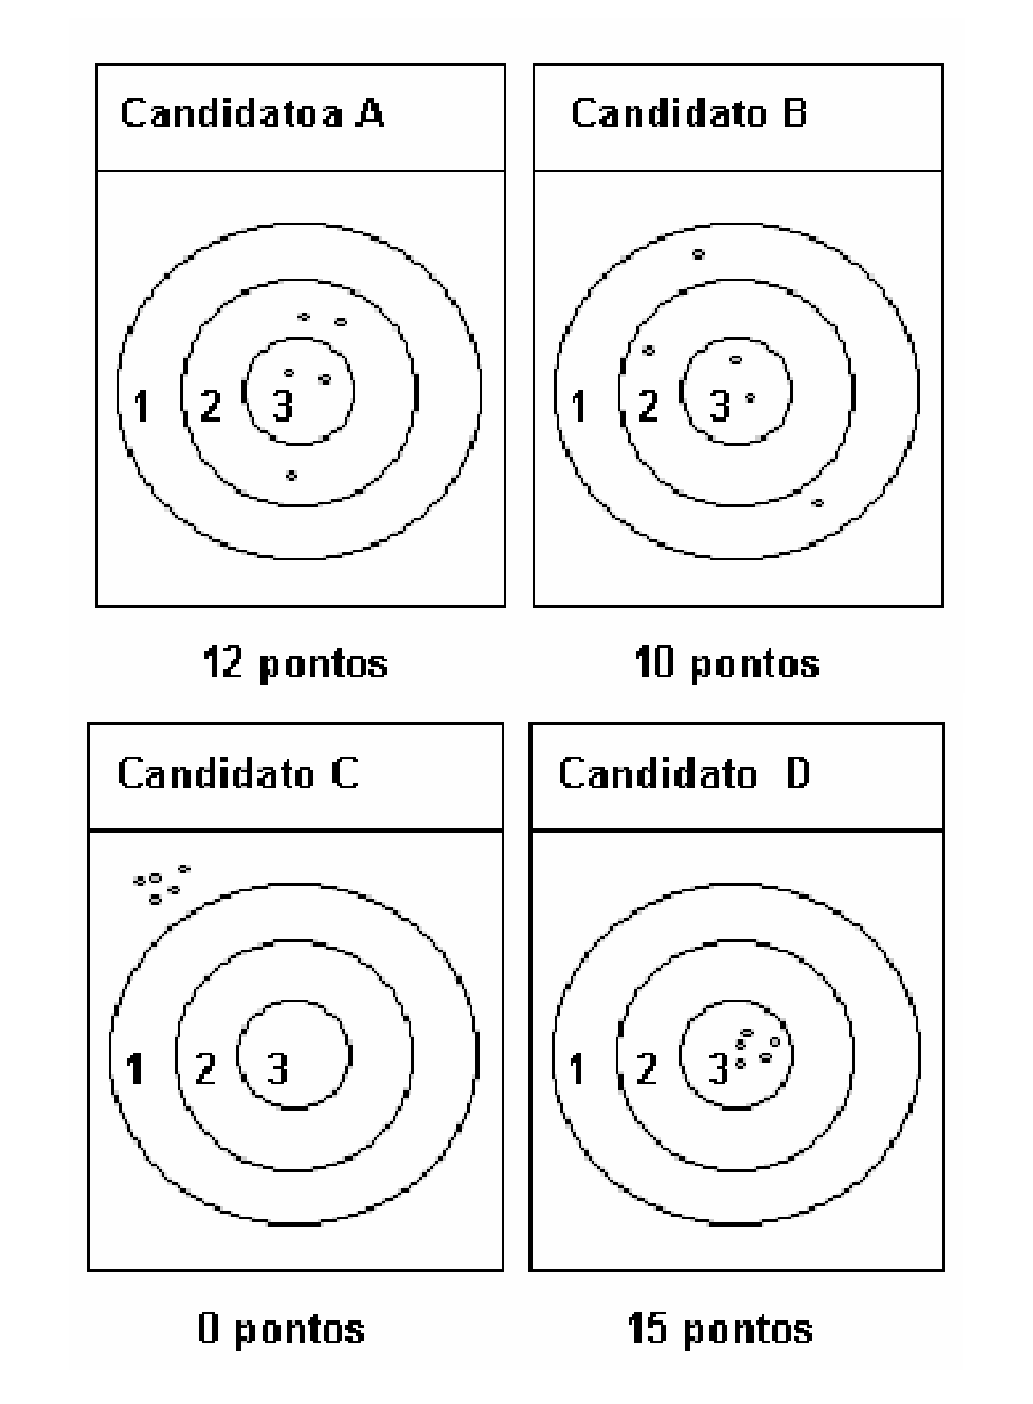
\includegraphics[scale=0.6]{figures/disp.eps}\\
  \vspace{-0.6cm}
  \caption{Exemplo Prático sobre Dispersão ou Variabilidade dos Dados}\label{esquematabela}
  }
\end{figure}

\newpage

O candidato mais "eficiente", em principio, deve corresponder àquele que tiver a maior média de pontos por tiro, o que nos conduz ao candidato D, que obteve uma média de 15/5 = 3 pontos/tiro.  Entretanto, verifica-se com uma simples inspeção dos alvos mostrados que o ("vesguinho") candidato C tem alguma chance de se constituir em um bom representante, mesmo com média de 0 pontos/tiro, após corrigirmos defeitos de sua visão, uma vez que ele mostrou ter uma pontaria muito "certeira"(!).  Pelos exemplos mostrados acima, vemos a necessidade de medidas complementares, visando a uma melhor análise da dispersão ou variabilidade dos resultados numéricos.\vskip0.3cm



Todas as medidas citadas têm um mesmo objetivo principal, ou seja, a quantificação da dispersão ou homogeneidade dos elementos das séries, permitindo dessa forma a comparação entre as mesmas no que a isso diz respeito. A série mais homogênea de todas é aquela cujos elementos são todos iguais entre si, o que nos leva à nulidade de todas as medidas de dispersão citadas acima. Observou-se dessa forma que, tão homogênea quanto à equipe de futebol que vence todas as partidas que disputa, é a equipe que perde também todas as suas partidas. Pode-se, em princípio, afirmar que, entre duas ou mais séries, a mais homogênea (ou menos dispersa) é aquela que apresenta a menor medida de dispersão, medida essa escolhida convenientemente.\vskip0.3cm

Em suma, o grau aos quais os dados numéricos tendem a dispersar-se em torno de um valor médio chama-se variação ou dispersão dos dados. Elas permitem se identificar até que ponto os resultados se concentram ou não ao redor da tendência central de um conjunto de observações.\vskip0.3cm

Dispõe-se de várias medidas de dispersão ou de variação, sendo as mais comuns, a amplitude total, o desvio médio, a amplitude semi-interquartílica, a variância, o desvio padrão, o erro padrão e o coeficiente de variação, cada um expressando diferentes formas de se quantificar a tendência que os resultados de um experimento aleatório têm de se concentrarem ou não em determinados valores (quanto maior a dispersão, menor a concentração e vice-versa).




\subsection{Desvio Médio (DM)}

\begin{equation}\label{dn}
    DM= \left[  \frac{\sum_{i=1}^{n}|(x_{i}-\bar{X})|}{n} \right]
\end{equation}

\newpage 

\subsection{Variância ($S^{2}$) de Dados Brutos}

A variância amostral de um conjunto de dados $x_{1},x_{2},\ldots,x_{n}$ , é assim definida:

\begin{eqnarray}\nonumber
S^{2} = \left[ \frac{(x_{1}-\bar{X})^{2}+(x_{2}-\bar{X})^{2}+\ldots+(x_{n}-\bar{X})^{2}}{n-1} \right]
    & = &  \\
    \left[ \frac{\sum_{i=1}^{n}(x_{i}-\bar{X})^{2}}{n-1} \right]  & = &  \\ \nonumber
    \left[ \frac{\sum_{i=1}^{n}x_{i}^{2}-\frac{(\sum_{i=1}^{n}x_{i})^{2}}{n}}{n-1} \right] &  &
\end{eqnarray}


\subsection{Variância ($S^{2}_{t}$) de Dados Tabulados}


\begin{eqnarray}\nonumber
S^{2} = \left[ \frac{(x_{1}-\bar{X})^{2}f_{1}+(x_{2}-\bar{X})^{2}f_{2}+\ldots+(x_{n}-\bar{X})^{2}f_{n}}{n-1} \right]
    & = &  \\
    \left[ \frac{\sum_{i=1}^{n}(x_{i}-\bar{X})^{2}f_{i}}{n-1} \right]  & = &  \\ \nonumber
    \left[ \frac{\sum_{i=1}^{n}x_{i}^{2}f_{i}-\frac{(\sum_{i=1}^{n}x_{i}f_{i})^{2}}{n}}{n-1} \right] &  &
\end{eqnarray}



\subsection{Variância Aparada ($S_{\alpha}^{2}$)}

Uma medida ainda mais elaborada de dispersão é conhecida como "Variância Aparada" (trimmed variance). A idéia, como para a "média aparada", é omitir uma proporção dos maiores e menores valores e calcular o análogo da variância amostral:

\begin{equation}\label{varAparada}
    S_{\alpha}^{2} = \left[\frac{1}{n-2k}\right]\sum_{i=k+1}^{n-k}(X_{i}-\bar{X}_{\alpha})^{2}
\end{equation}


Onde k é o inteiro mais próximo de $\alpha n$. Veja que é feita a média do quadrado dos desvios entre o valor e as médias aparadas consistentes (de acordo com a \label{aparada}). A variância aparada é algumas vezes multiplicada por um fator de ajuste para fazê-la mais consistente com a variância amostral ($S^{2}$).


\subsection{Desvio Padrão (DP)}

Definido como a raiz quadrada positiva da variância, o desvio-padrão exerce grande vantagem sobre a variância, já que ele é apresentado na mesma unidade de medida dos dados brutos. Trata-se da mais importante das medidas de variabilidade, onde indica a dispersão média absoluta dos dados em torno da própria média aritmética. O desvio-padrão pode ser assim obtido de duas maneiras:\vskip0.3cm

Para dados brutos, dp será

\begin{equation}\label{dp}
    DP= \sqrt{\frac{\sum_{i=1}^{n}(x_{i}-\bar{X})^{2}}{n-1}} = \sqrt{S^{2}}
\end{equation}

Já para dados tabulados, ficará

\begin{equation}\label{dp}
    DP= \sqrt{\frac{\sum_{i=1}^{n}(x_{i}-\bar{X})^{2}f_{i}}{n-1}} = \sqrt{S^{2}}
\end{equation}

\subsection{Coeficiente de Variação (CV)}

O coeficiente de variação ou coeficiente de variabilidade CV é uma medida de dispersão relativa, e útil para comparação, em termos relativos, do grau de concentração, em torno da média, de séries distintas.\vskip0.3cm 

Devido ser um número adimensional permite a comparação de séries de variáveis com unidades diferentes. Assim, o CV é a razão percentual entre o desvio padrão e a média aritmética, ou seja, pode-se caracterizar a dispersão ou variabilidade dos dados em termos relativos ao seu valor médio, sendo representada por:


\begin{equation}\label{CV}
    CV= \left[ \frac{S}{\bar{X}} \right]*100
\end{equation}

Costuma-se usar  a seguinte interpretação para o CV:

\begin{itemize}
\item até $15\%$ variação pequena;
\item $15\%$ a $30\%$ variação média;
\item de $30\%$ ou mais, variação grande; 
\end{itemize}

\newpage

\section{Medidas de Ordenação ou Separatrizes}
\subsection{Quartis $(Q_{i})$}






Quartis são medidas que dividem (separam) uma amostra (ou coleção) de dados de tipo quantitativo (ou qualitativo ordinal) ordenada em 4 partes iguais (FEIJOO, 2010).



\begin{enumerate}
  \item[{1)}] O 1º Quartil ou quartil inferior, representado por ($Q_{1}$) ou ($Q_{0,25}$), é o valor tal que pelo menos 25\% dos dados são não maiores do que ele e pelo menos 75\% dos dados são não menores do que ele;


  
  \item[{2)}] No 2º Quartil ($Q_{2}$), 50\% dos elementos estarão abaixo dele e 50\%, acima. Observe então que o 2º Quartil é igual à Mediana.
  \item[{3)}] No 3º Quartil ($Q_{3}$), 75\% dos elementos estarão abaixo dele e 25\%, acima.
  \vskip0.3cm
 \item[{4)}] No 4º Quartil ($Q_{4}$), 100\% dos elementos estarão resumidos. Nota-se que o 4º quartil é igual a média artimética.
\end{enumerate}


Para o cálculo do quartil utilizam-se os seguintes passos.



\begin{enumerate}

\item [{1°)}] Ordena-se os dados do menor para o maior;
\item [{2°)}] Encontra-se a frequência acumulada da distribuição;
\item [{3°)}]Calcula-se a posição do quartil na tabela.
$$ P_{(q_{i})} = \left[ \frac{(i \times n)}{4}  \right] $$
\item [{4°)}] Posteriormente, marca-se na tabela a posição pela frequência acumulada, para identificar em qual classe estará o quartil.
\item [{5°)}] Em seguida aplica-se a fórmula do quartil
\end{enumerate}

\begin{equation}\label{}
    Q_{1}= l_{q_{i}}+\left[\frac{P_{i}-FAA}{f_{q_{1}}}\right]\times h_{1}
\end{equation}

 onde

 \begin{itemize}
   \item $l_{q_{i}}=$ é o limite inferior da classe do quartil de ordem i;
   \item $FAA=$ È a freqüência acumulada anterior da classe do quartil de ordem i;
   \item $f_{q_{i}}=$ È a freqüência simples da classe do quartil de ordem i;
   \item $h_{i}=$ é o intervalo de classe;
 \end{itemize}




\subsection{Decis $(D_{i})$}

Dividem uma Distribuição de freqüência em 10 partes iguais.


\begin{enumerate}
  \item[{1)}] No $1º$ Decil ($D_{1}$), 10\% dos elementos estarão abaixo dele e 90\%, acima.
  \item[{2)}] No $2º$ Decil ($D_{2}$), 20\% dos elementos estarão abaixo dele e 80\%, acima.
  \item[{3)}] No $3º$ Decil ($D_{3}$), 30\% dos elementos estarão abaixo dele e 70\%, acima.
  \item[{4)}] $\ldots \ldots \ldots \ldots \ \ \  \ldots \ldots \ldots \ldots \ \ \  \ldots \ldots \ldots \ldots \ \ \  \ldots \ldots \ldots \ldots \ \ \ldots \ldots \ldots \ldots$
 \item[{5)}] No $10º$ Decil ($D_{10}$), 100\% dos elementos estão resumidos. Observe então que o $10º$ decil é igual a média artimética.
\end{enumerate}

\begin{enumerate}
\item [{1)}]Calcula-se primeira a posição do decil na tabela.
$$ P_{(d_{i})} = \left[ \frac{(i \times n)}{10} \right] $$
\item [{2)}] Posteriormente, marca-se na tabela a posição pela frequência acumulada, para identificar em qual classe estará o decil.
\item [{3)}] Em seguida aplica-se a fórmula do decil
\end{enumerate}

\begin{equation}\label{}
    D_{1}= l_{d_{i}}+\left[\frac{P_{d_{i}}-FAA}{f_{d_{1}}}\right]\times h_{1}
\end{equation}

 onde

 \begin{itemize}
   \item $l_{d_{i}}=$ é o limite inferior da classe do decil de ordem i;
   \item $FAA=$ È a freqüência acumulada anterior da classe do decil de ordem i;
   \item $f_{d_{i}}=$ È a freqüência simples da classe do decil de ordem i;
   \item $h_{i}=$ é o intervalo de classe;
 \end{itemize}



\subsection{Percentis $(P_{i})$}

Dividem uma Distribuição de freqüência em 100 partes iguais. Então:


\begin{enumerate}
  \item[{1)}] No $1º$ Percentil ($P_{1}$), 1\% dos elementos estarão abaixo dele e 99\% estarão acima.
  \item[{2)}] No $2º$ Percentil ($P_{2}$), 2\% dos elementos estarão abaixo dele e 98\% estarão acima.
  \item[{3)}] No $3º$ Percentil ($P_{3}$), 3\% dos elementos estarão abaixo dele e 97\% estarão acima.
   \item[{4)}] $\ldots \ldots \ldots \ldots \ \ \  \ldots \ldots \ldots \ldots \ \ \  \ldots \ldots \ldots \ldots \ \ \  \ldots \ldots \ldots \ldots \ \ \ldots \ldots \ldots \ldots$
  \item[{5)}] No $99º$ Percentil ($P_{99}$), 99\% dos elementos estarão abaixo dele e 1\% estarão acima.
   \item[{6)}] No $100º$ Percentil ($P_{100}$), 100\% dos elementos estão resumidos. Observe então que o $100º$ Percentil é igual a média artimética.
\end{enumerate}



\begin{enumerate}
\item [{1)}]Calcula-se primeira a posição do percentil na tabela.
$$ P_{(p_{i})} = \left[ \frac{(i \times n)}{100} \right] $$
\item [{2)}] Posteriormente, marca-se na tabela a posição pela frequência acumulada, para identificar em qual classe estará o percentil.
\item [{3)}] Em seguida aplica-se a fórmula do percentil
\end{enumerate}

\begin{equation}\label{}
    P_{p_{i}}= l_{p_{i}}+\left[\frac{P_{p_{i}}-FAA}{f_{p_{i}}}\right]\times h_{1}
\end{equation}

 onde

 \begin{itemize}
   \item $l_{p_{i}}=$ é o limite inferior da classe do percentil de ordem i;
   \item $FAA=$ È a freqüência acumulada anterior da classe do percentil de ordem i;
   \item $f_{p_{i}}=$ È a freqüência simples da classe do percentil de ordem i;
   \item $h_{i}=$ é o intervalo de classe;
 \end{itemize}



\section{Medidas de Forma, Enviesamento ou Assimetria }

\inic Embora sejam menos utilizadas na prática que as medidas de posição e
dispersão, as medidas de assimetria (\textit{skewness}) e curtose são úteis para
identificar modelos probabilísticos para análise inferencial.

\inic As medidas de assimetria e curtose são as que restam para complementarmos o quadro das estatísticas descritivas, que proporcionam, juntamente com as medidas de posição e de dispersão, a descrição e compreensão completas da distribuição de freqüências estudadas.\vskip0.3cm

Assimetria, como próprio nome insinua, significa desvio ou afastamento, ou seja, é o grau de desvio da simetria de uma distribuição ou afastamento de informação de uma curva de freqüência.\vskip0.3cm




%$$ b=\frac{1}{n}\sum_{i=1}^{n}\left[\frac{x_{i}-\bar{X}}{s}\right]^{2} $$

Uma medida usada muito freqüentemente para avaliar o grau de assimetria ou de deformação de uma distribuição e o coeficiente sugerido por Karl Pearson, o qual se calcula mediante as seguintes expressões:

\begin{enumerate}
  \item [{1)}]Primeiro Coeficiente de Assimetria de Pearson
  \begin{equation}\label{assimetria}
    AS = \left[ \frac{(Media-Moda)}{(Desvio-Padrao)} \right] = \left[  \frac{(\bar{X}-M_{o})}{S_{x}} \right]
\end{equation}
  \item [{2)}]Segundo Coeficiente de Assimetria de Pearson
  \begin{equation}\label{assimetria}
    AS = \left[ \frac{(Q_{3}+Q_{1}-2M_{e})}{(Q_{3}-Q_{1})} \right]
\end{equation}
    ou
 \begin{equation}
    AS = \left[ \frac{3(\bar{X}-M_{e})}{S_{x}} \right]
\end{equation}
\end{enumerate}






\textbf{Escala de Assimetria}

\begin{enumerate}
\item $|AS| =0$ a distribuição é Simétria
\item $|AS| < 0,15$ a Assimetria é Pequena
\item $0,15 < |AS| <1$ a Assimetria é Moderada
\item $|AS| > 1$ a Assimetria é Elevada
\end{enumerate}


\newpage 

Em um conjunto de dados, a mediana, a moda e a média
não necessariamente devem apresentar o mesmo valor. Uma
informação importante é que a mediana não é influenciada pelos valores extremos. Comparando os resultados encontrados para uma amostra em relação às medidas de posição estudadas e verificando a inter-relação entre elas, você pode concluir que seus valores podem nos dar um indicativo da natureza da distribuição dos dados, em função das regras definidas a seguir:


\begin{itemize}
\item Se a $\bar{X}=media$ for maior que a $\tilde{X}=mediana$ e maior que a Moda então a distribuição é assimétrica a direita (positiva), ou seja, os dados estão mais concentrados a direita.  	
\item Se a $\bar{X}$ for igual a $\tilde{X}$ e igual a moda então a distribuição é simétrica.
\item Se a $\bar{X}= media$ for menor que a $\tilde{X}= mediana$ e menor que a Moda então a distribuição é assimétrica a esquerda (negativa), ou seja, os dados estão mais concentrados a esquerda. 	
\end{itemize}

As medidas de tendência  central possuem algumas vantagens e desvantagens. A média possue a vantagem de Refletir cada valor observado na distribuição, e a desvantagem de ser influenciada por valores extremos. Já a mediana é menos sensível a valores extremos do que a Média, porém, é Difícil de determinar para grande quantidade de dados. Enquanto que a moda tem maior quantidade de valores concentrados neste ponto, e não se presta a análise matemática.
 
\newpage 

\section{Medidas de Achatamento, Afilamento ou Curtose }

\inic Em alguns casos uma distribuição pode ter seus valores concentrados próximos da média tal que a distribuição tem um pico mais alto, em outros casos a distribuição pode ser plana. Assim, medidas do grau de agudez de uma distribuição são chamadas de coeficiente de curtose (SPIGEL et al, 2013). \vskip0.3cm

\inic A curtose ou excesso indica até que ponto a curva de freqüências de uma distribuição se apresenta mais afilada ou mais achatada do que uma curva-padrão, denominada curva normal.\vskip0.3cm

\inic A medida de curtose é o grau de achatamento de uma distribuição, considerando usualmente em relação a uma distribuição normal. De acordo com o grau de curtose, podemos ter três tipos de curvas de freqüência: \textbf{Mesocúrtica}, \textbf{Leptocúrtica} e \textbf{Platicúrtica}.\vskip0.3cm

\begin{itemize}
\item Quando a distribuição apresenta uma curva de frequência mais fechada (mais aguda em sua parte superior), ela é denominada Leptocúrtica (Lepto = Delgado, Alongado, Magro, etc).
\item A distribuição de referência (Distribuição Normal) é denominada Mesocúrtica (Meso = Meio, Central, etc).
\item Quando a distribuição apresenta uma curva de frequência mais aberta (mais achatada em sua parte superior), ela é denominada Platicúrtica (Plato = Chato, Plano, Largo, etc).
\end{itemize}

Para avaliar o grau de curtose de uma curva ou distribuição de freqüências, usa-se o Coeficiente Percentílico de Curtose (K):

\begin{equation}\label{curtose}
    K = \left[ \frac{(Q_{3}-Q_{1})}{2(D_{9}-D_{1})} \right]
\end{equation}

Onde

\begin{itemize}
  \item $Q_{1}$ e $Q_{3}$  = é o primeiro e terceiro quartil;
  \item $D_{1}$ e $D_{9}$  = é o primeiro e nono decil;
   \end{itemize}

\vskip0.3cm

Sendo que existe um caso particular e a fórmula \ref{curtose} pode ser substituída
pelos percentis $P_{90}=D_{9}$ e $P_{10}=D_{1}$, quando for o caso.




\vskip0.3cm
Uma outra forma de representar o coeficiente de Curtose é da seguinte maneira

\begin{equation}\label{curtose2}
    K= \left[ \frac{C}{D_{9}-D_{1}} \right]
\end{equation}

onde o C é chamado de amplitude semi-interquartilica

\begin{equation}\label{curtose2}
    C= \left[ \frac{Q_{3}-Q_{1}}{2} \right]
\end{equation}


\textbf{Escala de Curtose}

\begin{enumerate}
\item Se $K = 0,263 \Rightarrow$  A curva correspondente à distribuição de frequências é \textbf{Mesocúrtica};
\item Se $K < 0,263 \Rightarrow$  A curva correspondente à distribuição é concentrada ao redor da média, ou seja, é mais pontiaguda ou afunilada e menos dispersa, sendo classificada de \textbf{Leptocúrtica};
\item Se $K > 0,263 \Rightarrow$ A curva correspondente à distribuição de frequência é mais dispersa ou Achatada, classificada de \textbf{Platicúrtica};
\end{enumerate}

\setcounter{chapter}{6} \chapter{Referências Bibliográficas}

BARBETTA, P. A. Estatística aplicada às ciências sociais. 7. ed. Florianópolis: Editora UFSC, 2010.\vskip0.3cm

BOISSEL, J. P. Planning of clinical trials. J Intern Med 2004; 255: 427-38.\vskip0.3cm

BROMAN, Karl, and Kara Woo. 2017. “Data Organization in Spreadsheets.” The American Statistician 72 (1): 2–10. https://doi.org/10.1080/00031305.2017.1375989.\vskip0.3cm

CAMEY, S. A.; NUNES, L. N.; CRUZ, L. N. Beanplot Uma Nova Ferramenta Gráfica. Clinical and Biomedical Research, [S. l.], v. 30, n. 2, 2010.\vskip0.3cm

CRONBACH, L. J. Coefficient alpha and the internal structure of test. Psychometrika, v. 16, n. 3, p. 297-334, 1951.\vskip0.3cm

Dantas, C. A. B. Probabilidade: Um Curso Introdutório. Ed.
USP, São Paulo, 1997.\vskip0.3cm


ECHEVESTE, Simone; BITTENCOURT, Hélio; BAYER, Arno; ROCHA, Josy. Educação estatística: perspectivas e desafios. Acta Scientiae, Canoas, v. 7, n. 1, p. 103-109, jan./jun, 2005.\vskip0.3cm


FELLER, W. Introdução a Teoria das Probabilidades e suas
Aplicações. Parte 1°: Espaços Amostrais Discretos, Edgard Blucher. São Paulo, 1976.\vskip0.3cm

FEIJOO, A. M. L. C. A pesquisa e a estatística na psicologia e na educação. Rio de Janeiro:
Centro Edelstein de Pesquisas Sociais, 2010, 109p. ISBN: 978-85-7982-048-9.\vskip0.3cm


FEIJOO, AMLC. Medidas separatrizes. In: A pesquisa e a estatística na psicologia e na educação
[online]. Rio de Janeiro: Centro Edelstein de Pesquisas Sociais, 2010, pp. 28-30. ISBN: 978-85-7982-048-9.\vskip0.3cm



GAL, I. Statistical tools and statistical literacy: the case of the average. Teaching
Statistics, 17(3), 97-99, 1995.\vskip0.3cm

HIEBERT, J. e LEFEVRE, P. Conceptual and procedural knowledge in mathematics: an
introductory analysis. In J. Hiebert (Ed.), Conceptual and procedural knowledge: the
case of mathematics, New Jersey, NJ: Lawrence Erlbaum, pp. 1-27, 1986.\vskip0.3cm

HOEL, P. G., PORT, S.C., STONE, C.S. Introdução a Teoria da Probabilidade. Rio de
Janeiro: Luter-Ciência, 1971.\vskip0.3cm

Hulley, Stephen B.; Cummings, Steven R.; Browner, Warren S. et al. Delineando a pesquisa clínica: uma abordagem epidemiológica. 2ª Ed. Porto Alegre: Artmed, 2003. p: 21-34.\vskip0.3cm

JAMES, B. R. . Probabilidade: Um curso em nível intermediário.
Projeto Euclides, IMPA, Rio de Janeiro, 1981. \vskip0.3cm


KENDALL, J. M. Designing a research project: randomised controlled trials and their principles. Emerg Med J. 2003 Mar;20(2):164-8. doi: 10.1136/emj.20.2.164. PMID: 12642531; PMCID: PMC1726034.\vskip0.3cm

KOWALSKI, B. R.; BENDER, C. Pattern Recognition. A powerfull Approch to Interpreting Chemical Data. Journal of the American Chemical Society, 94, 16, 5632–5639 (1972).\vskip0.3cm



LEOTTI, V. B.; MANCUSO, A. C. B.; BORGES, R. B.; DE JEZUS CASTRO, S. M.; HIRAKATA, V. N.; CAMEY, S. A. Modelagem estatística: Perguntas que você sempre quis fazer, mas nunca teve coragem. Clinical and Biomedical Research, [S. l.], v. 39, n. 4, 2019.\vskip0.3cm


MARCONI, Marina de Andrade e Lakatos, Eva Maria. Fundamentos de metodologia científica. 6ª ed. São Paulo, SP: Atlas, 2005.\vskip0.3cm

MEMÓRIA, J. M. P. Breve história da estatística, Embrapa Informação Tecnológica, Brasília, 2004, 111p. Texto para discussão, ISSN 1677-5473;21. \vskip0.3cm

MEYER, P. L. Probabilidade: Aplicações e Estatística. 2 ed.
Rio de Janeiro: Livros Técnicos e Científicos. Editora S.A. ,
1984.\vskip0.3cm


MOSLEY, Hugh \& MAYER, Antje. Benchmarking National Labour Market
Performance: a Radar Chart Approach. Berlin, Wissenschaftszentrum Berlin
für Sozialforschung Discussion Paper March 1999 ISSN Nr. 1011-9523, March
1999.\vskip0.3cm


PADOVANI, Carlos Roberto. Bioestatística. São Paulo, Cultura Acadêmica:
Universidade Estadual Paulista, Pró-Reitoria de Graduação, 2012.\vskip0.3cm

RAO, C. R. Linear statistical inference and its applications. New York: Wiley, 1973.\vskip0.3cm

RAO, C. R. Statistics: A technology for the millenium. International Journal of Mathematical and Statistics Sciences, Brasília, v. 8, n. 1, p. 5-25, 1999.\vskip0.3cm

TUKEY, J. W. Exploratory data analysis. Reading: Addison–Wesley, 1977.\vskip0.3cm

SNEDECOR, G. W. Statistical methods applied to experiments in agriculture and biology. Ames: The Iowa State College Press, 1937. \vskip0.3cm

STIGLER, S. M. The history of statistics: the measurement of uncertainty before 1900. Cambridge, MA: Harvard University Press, 1986. \vskip0.3cm

STUDENT. The probable error of a mean. Biometrika, London, v. 6, p. 1-25, 1908a.\vskip0.3cm

STUDENT. Probable error of a correlation coefficient. Biometrika, London, v. 6, p. 302-310, 1908b.\vskip0.3cm

STEINS, C. E; LOESCH, C. Estatística Descritiva e Teoria das Probabilidades, 2011 série Didática, EDFURB.\vskip0.3cm

SILVA, Edna Lúcia da. e Menezes, Estera M. Metodologia da pesquisa e elaboração de dissertação. 3ª ed. Florianópolis: Laboratório de Ensino a Distância da UFSC, 2001.\vskip0.3cm

SILVA, Cassandra Ribeiro de O. Metodologia e organização do projeto de pesquisa: guia prático. Fortaleza, CE: Editora da UFC, 2004.\vskip0.3cm

ROSS, S. A. First Course in Probability. 3 ed. New York:
McMillan Publishing Company, 1988.\vskip0.3cm


WHIPPLE, George Chandler. Vital Statistics: An Introduction to the Science of Demography, 1923. 








%\setcounter{chapter}{6} \chapter{Referências Bibliográficas}

BARBETTA, P. A. Estatística aplicada às ciências sociais. 7. ed. Florianópolis: Editora UFSC, 2010.\vskip0.3cm

BOISSEL, J. P. Planning of clinical trials. J Intern Med 2004; 255: 427-38.\vskip0.3cm

BROMAN, Karl, and Kara Woo. 2017. “Data Organization in Spreadsheets.” The American Statistician 72 (1): 2–10. https://doi.org/10.1080/00031305.2017.1375989.\vskip0.3cm

CAMEY, S. A.; NUNES, L. N.; CRUZ, L. N. Beanplot Uma Nova Ferramenta Gráfica. Clinical and Biomedical Research, [S. l.], v. 30, n. 2, 2010.\vskip0.3cm

CRONBACH, L. J. Coefficient alpha and the internal structure of test. Psychometrika, v. 16, n. 3, p. 297-334, 1951.\vskip0.3cm

Dantas, C. A. B. Probabilidade: Um Curso Introdutório. Ed.
USP, São Paulo, 1997.\vskip0.3cm


ECHEVESTE, Simone; BITTENCOURT, Hélio; BAYER, Arno; ROCHA, Josy. Educação estatística: perspectivas e desafios. Acta Scientiae, Canoas, v. 7, n. 1, p. 103-109, jan./jun, 2005.\vskip0.3cm


FELLER, W. Introdução a Teoria das Probabilidades e suas
Aplicações. Parte 1°: Espaços Amostrais Discretos, Edgard Blucher. São Paulo, 1976.\vskip0.3cm

FEIJOO, A. M. L. C. A pesquisa e a estatística na psicologia e na educação. Rio de Janeiro:
Centro Edelstein de Pesquisas Sociais, 2010, 109p. ISBN: 978-85-7982-048-9.\vskip0.3cm


FEIJOO, AMLC. Medidas separatrizes. In: A pesquisa e a estatística na psicologia e na educação
[online]. Rio de Janeiro: Centro Edelstein de Pesquisas Sociais, 2010, pp. 28-30. ISBN: 978-85-7982-048-9.\vskip0.3cm



GAL, I. Statistical tools and statistical literacy: the case of the average. Teaching
Statistics, 17(3), 97-99, 1995.\vskip0.3cm

HIEBERT, J. e LEFEVRE, P. Conceptual and procedural knowledge in mathematics: an
introductory analysis. In J. Hiebert (Ed.), Conceptual and procedural knowledge: the
case of mathematics, New Jersey, NJ: Lawrence Erlbaum, pp. 1-27, 1986.\vskip0.3cm

HOEL, P. G., PORT, S.C., STONE, C.S. Introdução a Teoria da Probabilidade. Rio de
Janeiro: Luter-Ciência, 1971.\vskip0.3cm

Hulley, Stephen B.; Cummings, Steven R.; Browner, Warren S. et al. Delineando a pesquisa clínica: uma abordagem epidemiológica. 2ª Ed. Porto Alegre: Artmed, 2003. p: 21-34.\vskip0.3cm

JAMES, B. R. . Probabilidade: Um curso em nível intermediário.
Projeto Euclides, IMPA, Rio de Janeiro, 1981. \vskip0.3cm


KENDALL, J. M. Designing a research project: randomised controlled trials and their principles. Emerg Med J. 2003 Mar;20(2):164-8. doi: 10.1136/emj.20.2.164. PMID: 12642531; PMCID: PMC1726034.\vskip0.3cm

KOWALSKI, B. R.; BENDER, C. Pattern Recognition. A powerfull Approch to Interpreting Chemical Data. Journal of the American Chemical Society, 94, 16, 5632–5639 (1972).\vskip0.3cm



LEOTTI, V. B.; MANCUSO, A. C. B.; BORGES, R. B.; DE JEZUS CASTRO, S. M.; HIRAKATA, V. N.; CAMEY, S. A. Modelagem estatística: Perguntas que você sempre quis fazer, mas nunca teve coragem. Clinical and Biomedical Research, [S. l.], v. 39, n. 4, 2019.\vskip0.3cm


MARCONI, Marina de Andrade e Lakatos, Eva Maria. Fundamentos de metodologia científica. 6ª ed. São Paulo, SP: Atlas, 2005.\vskip0.3cm

MEMÓRIA, J. M. P. Breve história da estatística, Embrapa Informação Tecnológica, Brasília, 2004, 111p. Texto para discussão, ISSN 1677-5473;21. \vskip0.3cm

MEYER, P. L. Probabilidade: Aplicações e Estatística. 2 ed.
Rio de Janeiro: Livros Técnicos e Científicos. Editora S.A. ,
1984.\vskip0.3cm


MOSLEY, Hugh \& MAYER, Antje. Benchmarking National Labour Market
Performance: a Radar Chart Approach. Berlin, Wissenschaftszentrum Berlin
für Sozialforschung Discussion Paper March 1999 ISSN Nr. 1011-9523, March
1999.\vskip0.3cm


PADOVANI, Carlos Roberto. Bioestatística. São Paulo, Cultura Acadêmica:
Universidade Estadual Paulista, Pró-Reitoria de Graduação, 2012.\vskip0.3cm

RAO, C. R. Linear statistical inference and its applications. New York: Wiley, 1973.\vskip0.3cm

RAO, C. R. Statistics: A technology for the millenium. International Journal of Mathematical and Statistics Sciences, Brasília, v. 8, n. 1, p. 5-25, 1999.\vskip0.3cm

TUKEY, J. W. Exploratory data analysis. Reading: Addison–Wesley, 1977.\vskip0.3cm

SNEDECOR, G. W. Statistical methods applied to experiments in agriculture and biology. Ames: The Iowa State College Press, 1937. \vskip0.3cm

STIGLER, S. M. The history of statistics: the measurement of uncertainty before 1900. Cambridge, MA: Harvard University Press, 1986. \vskip0.3cm

STUDENT. The probable error of a mean. Biometrika, London, v. 6, p. 1-25, 1908a.\vskip0.3cm

STUDENT. Probable error of a correlation coefficient. Biometrika, London, v. 6, p. 302-310, 1908b.\vskip0.3cm

STEINS, C. E; LOESCH, C. Estatística Descritiva e Teoria das Probabilidades, 2011 série Didática, EDFURB.\vskip0.3cm

SILVA, Edna Lúcia da. e Menezes, Estera M. Metodologia da pesquisa e elaboração de dissertação. 3ª ed. Florianópolis: Laboratório de Ensino a Distância da UFSC, 2001.\vskip0.3cm

SILVA, Cassandra Ribeiro de O. Metodologia e organização do projeto de pesquisa: guia prático. Fortaleza, CE: Editora da UFC, 2004.\vskip0.3cm

ROSS, S. A. First Course in Probability. 3 ed. New York:
McMillan Publishing Company, 1988.\vskip0.3cm


WHIPPLE, George Chandler. Vital Statistics: An Introduction to the Science of Demography, 1923. 








%\setcounter{chapter}{7} \chapter{Considerações Gerais}








%%%%%%%%%%%%%%%%%%%%%%%%%%%%%%%%%%%%%%%%%%%%%%%%%%%%
%%%                                              %%%
%%%             Backmatter                       %%%
%%%                                              %%%
%%%%%%%%%%%%%%%%%%%%%%%%%%%%%%%%%%%%%%%%%%%%%%%%%%%%

\is{some term| see {some other term}}
\il{some language| see {some other language}}
\issa{some term with pages}{some other term also of interest}
\ilsa{some language with pages}{some other lect also of interest} 
% There is normally no need to change the backmatter section
\backmatter
\phantomsection%this allows hyperlink in ToC to work
\printbibliography[heading=references] 
\cleardoublepage

\phantomsection 
\addcontentsline{toc}{chapter}{Index} 
\addcontentsline{toc}{section}{Name index}
\ohead{Name index} 
\printindex 
\cleardoublepage
  
\phantomsection 
\addcontentsline{toc}{section}{Language index}
\ohead{Language index} 
\printindex[lan] 
\cleardoublepage
  
\phantomsection 
\addcontentsline{toc}{section}{Subject index}
\ohead{Subject index} 
\printindex[sbj]
\cleardoublepage
 
\end{document} 

% you can create your book by running
% xelatex main.tex
%
% you can also try a simple 
% make
% on the commandline
